\documentclass[11pt]{book}
\usepackage{res_doc_log}
\usepackage[ruled]{algorithm2e}
\usepackage{algorithmic}
\usepackage{amsmath} 
\usepackage{graphicx}
\usepackage{tikz}
\usepackage{booktabs} 
\usepackage[numbers,sort]{natbib}
\usepackage{url} 
\usepackage{textcomp}
\usepackage{mathtools}
\usepackage{caption}
\usepackage{longtable}

\thesistitle{A combined resource allocation and epidemic model to evaluate UAV vaccine delivery and team allocation strategies for measles outbreak response}
\student{Dean Michael Matter}
\graduation{December}
\myyear{2019}
\frontmatter

%Study leader
\supervisor{Dr Linke Potgieter}

\begin{document}
\frontpage[honsbcom]{or}
\dominitoc 
\engabstract{
Humanitarian aid in developing countries is often faced with a wide array of challenges, one of which being the lack of sufficient and stable road infrastructure. In the context of an epidemic, this may result in inefficient outbreak responses such as the late delivery of vaccines. Unmanned aerial vehicles have emerged as a potential alternative to land-based delivery methods, and have been successfully used for an ever-increasing number of medical deliveries in recent years. In this project, the effectiveness of unmanned aerial vehicles for vaccine delivery (in comparison to land-based delivery) in the context of rural epidemic outbreaks (with a particular focus on measles epidemics), is evaluated, along with various vaccine and team allocation strategies.\\
A combined resource allocation and epidemic model is developed to simulate vaccine delivery during a measles outbreak. A network approach is followed in this simulation model, with the network consisting of local populations connected by the migration of individuals. The measles epidemic is simulated by using a compartmental model, which comprises of a system of difference equations for each local population, with a small proportion of each population migrating to other local populations daily. During each time step, optimised daily vaccine delivery schedules and team allocations are determined, by modelling each as a knapsack problem. The objective of each is to minimise the expected number of people exposed to measles, and consequently, minimise the number of measles-induced deaths. Heuristic approaches for resource allocation are also considered. It is clear from simulations that faster outbreak response has a large impact on the number of deaths prevented. Furthermore, finding optimised daily team allocations resulted in a 22.4\% reduction in simulated vaccine and delivery costs. Unmanned aerial vehicles are shown to be capable of meeting demand for vaccines in a simulated measles outbreak, and reduce costs and deaths when used instead of a land-based delivery network in areas with poor road infrastructure.
}

\mainmatter
\tableofcontents
%\listoffigures
%\listoftables

\listofsymbols
\begin{longtable}[c]{ll}
Symbol & Description \\ \hline
\endfirsthead
%
\endhead
%
$n$ & Number of locations in the network. \\
$\mathcal{T}$ & Number of days simulated. \\
$\mathcal{H}$ & Number of working minutes per day. \\
$\mathcal{N}$ & Total number of vaccination teams. \\
$\eta_{i,t}$ & Number of teams at location $i$ on day $t$. \\
$\psi_{i}$ & Number of vaccinations that each team in location $i$ can perform daily. \\
$\tau_{i,t}$ & Number of people present to be vaccinated, on day $t$ at location $i$. \\
$\nu_{i,t}$ & Number of vaccines on-hand on day $t$ at location $i$. \\
$v_{i,t}$ & Number of vaccinations performed on day $t$ at location $i$. \\
$\theta^{S}_{i,t}$ & Proportion of remaining unvaccinated population that is susceptible, \\ &on day $t$ at location $i$. \\
$\theta^{E_{72}}_{i,t}$ & Proportion of remaining unvaccinated population that has been exposed \\ &in the preceding 72 hours, on day $t$ at location $i$. \\
$\lambda_{S}$ & Vaccine success rate in susceptible individuals. \\
$\lambda_{E}$ & Vaccine success rate in individuals exposed for less than 72 hours. \\
$S_{i,t}$ & Number of susceptible individuals at location $i$ on day $t$. \\
$E_{i,t}$ & Number of exposed individuals at location $i$ on day $t$. \\
$I_{i,t}$ & Number of infectious individuals at location $i$ on day $t$. \\
$R_{i,t}$ & Number of recovered individuals at location $i$ on day $t$. \\
$V_{i,t}$ & Number of vaccinated individuals at location $i$ on day $t$. \\
$D_{i,t}$ & Number of deceased individuals at location $i$ on day $t$. \\
$\mathcal{D}_{i,j}$ & Distance by direct road between locations $i$ and $j$. \\
$\Delta_{i,j}$ & Euclidean distance between locations $i$ and $j$. \\
%$i^{*}$ & Location in the network at which the Distribution Centre is placed. \\
$T_{i,j}$ & Number of individuals moving from location $i$ to $j$ daily. \\
$m_{i,j}$ & Proportion of population at location $i$ moving to location $j$ daily. \\
$v'_{i,t}$ & Expected number of vaccines still required at location $i$ on day $t$. \\
$\delta_{d,i}$ & Total flight time for a UAV delivery from the Distribution Centre to location $i$. \\
$\delta_{v,i,j}$ & Total travel time between locations $i$ and $j$, by road. \\
$\mathcal{R}$ & Set of all vehicle delivery routes considered. \\
$\delta_{v,r_{k}}$ & Total travel time for a route $r_{k}$, by road. \\
$E^{*}_{x_{i},i,t+1}$ & Expected prevented exposures resulting from a delivery of $x_{i}$ vaccines to \\ &location $i$ on day $t$. \\
$E^{*}_{r_{k},t+1}$ & Expected prevented exposures resulting from deliveries of $v'_{i,t}$ vaccines to \\ &each location $i$ in route $r_{k}$, on day $t$. \\
$E^{*}_{\eta_{i,t},i,t+1}$ & Expected prevented exposures resulting from $n_{i,t}$ teams being assigned to \\ &location $i$, on day $t$.
\label{tab:symbols_list}\\
\end{longtable}


%\input{sub1_doc_example.tex}

\chapter{Introduction}
In recent years, Unmanned Aerial Vehicles (UAVs, or drones) have been developed rapidly and have been tested for a wide range of applications. One such application is in the field of humanitarian aid and epidemic response -- UAVs are already in regular use for the routine delivery of blood and medication, and research is being performed to investigate whether it is worthwhile and cost-effective to use them in emergency scenarios as well. In rural and hard-to-reach areas, UAVs can be particularly useful for delivery since they are not constrained by poor road networks, and can make a life-saving impact in the case of medical deliveries. This project investigates the potential usage of UAVs for the delivery of measles vaccines in a rural context such as this, in comparison to the existing land-based cold chain. Resource allocation strategies are also considered, to gain insight into potential improvements on current outbreak response efforts.

\section{Background}
\label{measles-background}
Measles is an extremely contagious disease caused by the measles virus, transmitted from infected to susceptible individuals, primarily through the air. It generally takes 10 to 14 days after exposure for the initial symptoms of measles infection to appear, followed by a rash 2 to 4 days thereafter. Subjects are contagious from roughly day 10 to day 18, and during this period, up to 90\% of unimmunized people they come into contact with will contract the measles virus from them \cite{cdc_2018}. 
In developing countries, particularly those whose citizens suffer from malnutrition, AIDS and Vitamin A deficiency, the death rate for measles cases is often as high as 10\%. This is nearly 100 times higher than in developed countries. This case-fatality rate can even rise to 30\%, particularly in hard-to-reach areas where large portions of the population have weak immune systems and have not yet been vaccinated \citep{world2017measles}. It is therefore imperative to prevent or control measles epidemics, particularly in developing countries.

\subsection{Measles epidemic prevention}
Fortunately, measles epidemics are preventable by vaccination, with a vaccine released in 1963. Prior to that, there were approximately 30 million cases and 2 million deaths worldwide every year, particularly in children and infants; almost 95\% of 15-year-olds would have been infected by measles before the vaccine's introduction \citep{world2017measles}.
The currently available vaccines are relatively cheap, and effective. From 2000 to 2015, the number of measles cases reduced by 75\%, and deaths reduced by 79\%. Globally in 2015, there were 35 cases per million people, and a total of 134\,200 deaths - a marked improvement from pre-1963. Vaccination immunises nearly all susceptible individuals, and can also be administered to patients within 72 hours of exposure to the virus to mitigate symptoms and reduce the severity of the infection \citep{world2017measles}. Outbreak response can thus include both post-exposure and pre-exposure vaccinations.

Despite these reductions in measles cases globally, vaccination of less developed nations has proven challenging due to limited healthcare and road infrastructure. 
After 2017, 85\% of children globally had received a first vaccination dose, with just 67\% having also received the second dose \citep{worldhealthorganization_2018}. 
An effective population coverage is only attained when 95\% of children under 15 years old are immune \cite{msf_2017}, and hence the current global vaccination levels are insufficient.
In 2015, there were an estimated 20.8 million infants worldwide (out of 141 million total births \citep{owidfertilityrate}) that did not receive the first vaccination dose - of which over 20\% were born in Nigeria, Ethiopia and the Democratic Republic of Congo (DRC) \citep{world2017measles}. 
Since many unvaccinated people are concentrated in hard-to-reach areas of developing nations, improved methods of reaching these susceptible individuals is a priority.

\subsection{Vaccine distribution challenges}
A major contributing factor to the poor vaccination rate in these and other developing countries is the lack of a proper distribution network through which to deliver vaccines and other supplies to vaccination sites. In many African countries, the majority of the transportation network consists of unpaved dirt roads, or poorly maintained tarmac. There are very few tunnels, bridges or highways, and these dirt roads often become impassable mud in rainy seasons, especially after persistent rains - which are common in equatorial African countries in particular. Even if roads are passable, it can take hours or days to deliver vaccines by road - which is often too slow of a response in the case of an outbreak or medical emergency.
This is a major problem because, ``just a third of Africans live within two kilometres of an all-season road" \citep{harris_2019}. That means two thirds of Africans are essentially unreachable during rainy seasons, and were an outbreak of any serious infectious disease to occur, there is no straightforward way to vaccinate people and curb the spread of the disease using the current cold chain. 

%The vaccine distribution network in many developing countries is antiquated and unnecessarily layered. These networks usually consist of a national Distribution Centre (DC) supplying regional DCs, which supply provincial DCs, which then supply district DCs. Finally, the district DCs deliver to the PODs \citep{humphreys_2011}.
%Instead, due to modern communications technology, much fewer layers are required - PODs can even communicate supply requirements directly with a single national DC. For the case of epidemic response, a smaller network with a single DC supplying PODs directly can often be implemented.

Balancing the vaccine inventory kept with vaccination teams is also highly challenging. Even with the assumption that all roads are passable year-round, demand for vaccines is uncertain. Excess stock causes increased cold storage costs and wastage (since vaccines have an expiry date), and a shortage of vaccines means that not enough people can be vaccinated. Since the cost of a dose of the measles vaccine is \$2.85 \cite{unicef_2019}, the cost of wastage can be significant. There is also often not enough cold storage space for vaccines at vaccination sites, particularly in the case of epidemic responses \citep{humphreys_2011}. On top of this, when roads become impassable due to weather or other factors, a complex, expensive and life-changing logistical challenge emerges.

\subsection{UAV delivery}
In recent years, UAVs have emerged as a possible alternative to the land-based cold chain for medical deliveries, with other applications including farming, warfare, firefighting, entertainment, and humanitarian aid, among others.
Specifically within the field of healthcare, there have already been attempts at UAV deliveries for medication, blood and vaccines.
Matternet, an American company, has used fully autonomous quadcopter UAVs in conjunction with Doctors Without Borders and UNICEF, to deliver medication in Haiti, the Dominican Republic, Switzerland, and New Guinea. Matternet, as well as UPS, DHL Parcel and Flirtey, have also recently embarked upon forays into routine UAV deliveries of medical supplies in developed countries as well. DHL Parcel and Flirtey's UAVs have reduced certain routine delivery times from 30 minutes to 8 minutes, and 90 minutes to 3 minutes, respectively \cite{scott2017drone}.
Finally, a US startup called Zipline currently delivers blood and vaccines routinely in parts of Rwanda, Ghana and Tanzania. Zipline's UAVs are fixed-wing instead of quadcopters, allowing a top speed of over 144km/h rather than 40km/h. Despite a slightly smaller payload capacity, Zipline's UAVs can service a much larger range than quadcopters (160km rather than 10-20km), and are therefore the UAVs that are assumed to be used for the purposes of this project.

Unfortunately, the use of UAVs for medical deliveries is not without caveats. There is the serious risk of collisions with airplanes and, thus, appropriate airspace legislation is required before regular deliveries can take place. There are other concerns regarding mechanical reliability, payload dropoff methods, and theft. Specifically within the context of vaccine delivery, major challenges include controlling the temperature at which vaccines are transported at throughout the flight, as well as a limited delivery range and small payload. However, should some of these challenges be overcome, the use of UAVs for vaccine delivery appears to be highly promising.

\section{Problem description}
Planned, routine vaccination campaigns, particularly against contagious diseases such as measles, are a priority in many nations. However, more drastic action is required in the case of an epidemic. In response to a 2005 measles outbreak in the DRC, Doctors Without Borders (MSF) vaccinated 104\,549 children in two weeks, at 18 vaccination sites around the port town of Matadi \cite{msf_2006}. In such a rapid response, available response teams need to be promptly deployed in the network, and an efficient and reliable delivery network for vaccines needs to be established as quickly as possible. Currently, vaccines are delivered to vaccination sites by truck, motorbike, or even by foot - depending on the road quality and accessibility of the site. Sometimes rivers even need to be crossed in makeshift ferries \cite{msf_2017}. The World Health Organisation (WHO) mentions ``...optimal strategies for reaching hard-to-reach populations [for vaccination]" \cite{world2017measles} as an important aspect of measles intervention which Operations Research can assist with. To that end, this project will compare team allocation and delivery strategies, and evaluate the possibility of using UAVs to deliver vaccines in an outbreak response scenario.

More specifically, the research question under consideration is the following: In the case of a rural measles outbreak, are UAVs an efficient alternative vaccine delivery method (given capacity constraints), and which factors and resource allocation strategies contribute most to the success of an intervention?

\section{Scope of project}
In the scope of this project, the only disease considered is measles -- although this approach can easily be adapted to other diseases by changing parameters. This project only considers delivery networks using UAVs similar to those used by Zipline, since their UAVs can cover the furthest range. Since this range is large enough to include a city and surrounds, the delivery network is assumed to have only a single DC. The temperature at which the vaccines are transported and stored is not considered. Weather and seasonality do have an effect on the contagiousness of measles, but this effect is also not modelled in the scope of the project. The entire network of locations is assumed to be closed, with no migration into or out of the network. Finally, it is assumed that vaccination is the only intervention occurring in the epidemic, and that there is no impact of any other healthcare activities on the population.

\section{Project objectives}
The objectives that shall be followed to address the problem outlined are:

\textbf{Objective 1:} Perform a literature review, considering literature about epidemic modelling and simulation, to establish methods which can be implemented in this project. 

\textbf{Objective 2:} Develop a simulation model for the spread of measles across a network of interacting populations.

\textbf{Objective 3:} Develop a resource allocation model for the daily allocation of human and vaccine resources across the network.

\textbf{Objective 4:} Investigate potential resource allocation strategies, and the effect of factors such as setup delay on interventions.

\textbf{Objective 5:} Evaluate possible improvements to interventions, such as UAV delivery.

\section{Structure of this report}
Immediately following this introduction, a brief review of relevant literature is undertaken in Chapter 2. This is followed by a detailed discussion of the methodology used for the simulation, in Chapter 3. Chapter 4 follows, with a presentation and discussion of the results found using the aforementioned methodology. Finally, conclusions are drawn in Chapter 5, before a list of references and appendix.

%\chapter{Literature Summaries}
%
\subsection{Insights into controlling Ebola in west africa}
\cite{buyuktahtakin2018new} use a model to ``...determine the optimal amount, timing and location of resources that are allocated for controlling and infectious disease outbreak while accounting for its spatial spread dynamics." The purpose of the model was to minimize the total number of infections and fatalities under a limited budget and time period. They consider \emph{geographically varying} rates for disease transmission, as well as the movement of individuals between geographic regions, and varying treatment rates due to limited clinic capacities. A mixed-integer programming model is proposed, which minimises the number of infections and deaths due to Ebola, while considering the spread of the epidemic and the logistics required to control it. The migration of people within the risk area of the epidemic is also taken into account, as this can affect its spread.  Various classifications of the population are used in the model; Susceptible, Infected, Treated, Recovered, Dead, and Buried. The final classification is significant due to West African burial practices, which involve contact with the corpse during the burial procedure. \\
There is a risk to oversimplifying the modelling of spread of epidemic outbreaks by ignoring the spread of disease over geography, and the differing rates of treatment capacity. \cite[p.~2]{buyuktahtakin2018new} \\
``...treatment considerably lessens the disease’s impact, compared to the no-treatment case, regardless of the starting date"
``the cumulative number of treated individuals in- creases proportional to the available budget” \\
``In all cases, we observe that treatment considerably lessens the disease’s impact, compared to the no-treatment case, regardless of the starting date. However, the earlier the starting date of the intervention, the fewer the infections and funerals.” \\
``Our results have a one-to-one correspondence with the basic reproduction number, R 0 , which is defined as the expected number of secondary cases of a typical single infected individual during his or her entire infectious period, in a population which is entirely susceptible. If R 0 < 1, dis- ease transmission is not self-sustaining and is unable to generate a major epidemic. On the other hand, an epidemic is likely to occur whenever R 0 > 1. If $R_{0}$ = 1 , each existing infection is causing one new infection, and the disease will stay alive without epidemic.” \\
``This result shows that for each month of delay in intervention, the required optimal amount of budget to control the epidemic nearly doubles.”\\
``Although a significantly larger treatment budget is allocated in delayed-intervention cases, total infections and deaths by the end of the planning horizon are considerably larger compared to early treatment efforts”\\
``Our analysis suggests that in order to stop the spread of Ebola and consequently reduce fatalities, policymakers must focus primarily on reducing transmission and contact rates aside from the rapid introduction of treatment efforts”\\
``All results from the case study consistently show that early control reduces infection and fatalities considerably more compared to delayed intervention. While a late implementation of control intervention requires intense response efforts and a significantly larger treatment budget, it still leads to a substantially greater cumulative number of infections and deaths compared to the case when intervention is early.”\\

\subsection{Commonly used OR models for epidemiological modelling}
Methods of OR used for epidemiological modelling in the past, described by \cite{buyuktahtakin2018new}, include:
\begin{itemize}
    \item Compartmental model-based simulations - which can model disease dynamics fairly accurately, but can only consider a small number of intervention strategies. Further, simulations for optimization require a lot of computational power and time and use heuristics - which are not guaranteed to provide an optimal solution.
    \item Differential equation based models
    \item Resource allocation methods to minimise cost
    \item Network models
    \item Mathematical programming - including linear and integer programming, non-linear optimisation and stochastic programming. These methods can be useful because they analyse all intervention strategies and find the best possible one. These can be used in conjunction with simulation - epidemic spread and growth is simulated before being used as input in the model. These models are often used to find the best vaccination strategies.
    \item Facility location models - including maximal covering, optimal location-allocation and P-median allocation models
    \item Agent-based simulation - along with social networks, to model the interactions between people and transmission of the epidemic
\end{itemize}

\subsection{Wanying Article - on Anthrax attacks using Markov processes}
The model involves Markov processes and takes into account the progression of the anthrax disease in the medical and logistics response. \\
`` In particular, the approach allows us to capture dynamically the impact of different medical responses on the infected population. Dynamics are important because the time elapsed since the patient is infected till the moment he/she receives medical treatment has a major impact on the recovery rate, the survival rate and, therefore, on the number of deaths.” \citep{wanying2016modeling} \\
\textsc{Need to find disease stages for measles and work out at which point someone is infected and contagious, and use that in the model – cause drones need to get there quickly. Also, consider recovery or death rate at each point. } \\
``In other words, the main reason of the high death rate is that patients cannot get the medical help in time because of the limited logistics capacity and the short disease period.”\citep{wanying2016modeling} \\
``To sum up, it appears to us that, in all the cases, a large scale attack would require a very high dispensing antibiotics capacities, so the most effective way to reduce the number of causalities is to speed up the detection thus limiting the number of infected people."\citep{wanying2016modeling} \\

\subsection{Dasaklis - smallpox attack (disease progression model and LP for vaccine allocation)}
\citep{dasaklis2017emergency}
Transmission model is used for disease spread and dynamics, LP model for optimal distribution of vaccines to certain locations and populations. Some sensitivity analysis upon assumptions. \\
For smallpox, many people are susceptible since the disease is eradicated and routine vaccinations not needed. To what extent is this the same for measles? Also, vaccinations are risky – chance of illness and even death is considerable. Recommended strategy for vaccination in case of outbreak is targeted or ring vaccination – isolate and vaccinate close contacts. More and more people vaccinated if a high R0 basic reproduction number. \\
``From a logistical point of view,
the implementation of a broader vaccination campaign
should rely on the establishment of an emergency supply
chain and a series of decisions should be made regarding
the location, number and capacity of both the stockpile
centres and final Points of Dispensing (PODs), the
inventory level of medical supplies and commodities
held within these facilities as well as the replenishment
policies adopted, the assignment of these facilities to
serve certain sub-populations and, finally, the selection
of modes of distribution and relevant capacities.” \\
``In particular, the dynamics of the
spread of a smallpox outbreak and its interactions with
resource allocation decisions are considered. A modelling
approach is presented consisting of two modules. The
first module relates to disease’s progression, whereas the
second one relates to optimally distributing a set of supplies
(medical and ancillary) to affected sub-populations.” \\
``Although ring vaccination is highly recommended for
controlling a smallpox outbreak, it is questionable
whether such an intervention would yield optimal results
in the case of a large-scale bioterrorist attack” \\
``As the outbreak lasts several
weeks, birth/death processes have been excluded from
the disease progression model (they normally affect the
dynamics of endemic diseases over several years).” \\


\subsection{WHO Position Paper}
\citep{world2017measles}
``Increasing population immunity through vaccination is the most effective way to prevent outbreaks."

``There is no specific treatment for measles."

``In unimmunized or insufficiently immunized individuals, measles vaccine may be administered within 72 hours of exposure to measles virus to protect against disease." This reduces severity of symptoms and length of onset.
The standard vaccine dose is 0.5m$\ell$.
The vaccine needs to be stored below 8\textdegree C.
After a second vaccine dose, 95\% of children who did not become immune after their first vaccine dose become immune. But ``evidence indicates that a single dose
of correctly administered measles vaccine which results in seroconversion will afford lifelong protection for most healthy individuals."

Serious adverse affects to measles vaccination occur more frequently for multidose vials.

``Measles immunization saves high costs for the individuals
affected, their families and the national healthcare
system." Further, the measles vaccine is inexpensive.\\

``Programmatic
questions that should be addressed include: which
populations should be targeted for special immunization
efforts; optimal strategies for reaching hard-to-reach
populations, and adolescents and adults; how to
strengthen and enhance disease surveillance and
reporting; the best approaches to measuring vaccination
coverage; strategies to communicate the benefits of
measles vaccination and minimize vaccine hesitancy;
and the economic impact of the disease."\\


\chapter{Literature Review}
A brief review of relevant literature is undertaken in this chapter. In \S \ref{sec:lit_matSim}, various methods of modelling epidemics are presented and discussed. This is followed by a discussion of literature about vehicle routing problems in \S \ref{sec:lit_VRP}, with a particular focus on literature about vehicle routing problems involving UAVs. A discussion of resource allocation problems in epidemic response is given in \S \ref{sec:lit_VaccHumRes}, and the chapter is concluded with an overview of facility location problems relevant for the problem of selecting a distribution centre from which vaccines can be delivered by UAV.

\section{Mathematical and simulation modelling of infectious diseases}
\label{sec:lit_matSim}
Modelling infectious diseases can prove indispensable in saving lives by helping decision makers to understand epidemics better. There are a number of modelling methods which have been developed for this purpose.

\subsection{Compartmental models}
\label{sec:lit_SEIR}
In compartmental models, the affected population is divided into distinct categories. These models can use either discrete or continuous time steps, describing disease progression using difference equations and differential equations, respectively \cite{selvam_2015}. For the SEIR measles epidemic model (an adaptation of the SIR model), appropriate population categories are: \textit{Susceptible} (S), \textit{Exposed} (E), \textit{Infectious} (I), and \textit{Removed} (R) \cite{chitnis_2017}. Categories for \textit{Dead} (D), and \textit{Vaccinated} (V) can be included as well. The population progresses between categories in the model as described in Figure \ref{fig:lit_SEIR}. Note the assumption that only individuals in the S, E and R classes can be vaccinated, and only individuals in the I class can die and move to the D class.

\begin{figure}[ht!]{\textwidth}
    \centering
    \resizebox{0.5\textwidth}{!}{\input{SEIRVD.pdf_tex}}
    \caption{Progression of population between categories in the SEIR model.}
    \label{fig:lit_SEIR}
\end{figure}

The basic continuous-time SEIR model is described by the following system of differential equations \cite{IDM_2019, chitnis_2017}:
\begin{align*}
    \frac{dS}{dt} &= -\frac{\beta SI}{N} \\
    \frac{dE}{dt} &= \frac{\beta SI}{N} - \sigma E \\
    \frac{dI}{dt} &= \sigma E - \gamma I - \mu I\\
    \frac{dR}{dt} &= \gamma I + \mu I.
\end{align*}

This basic SEIR model requires transition rates $\beta, \sigma, \gamma \text{ and } \mu$, for movement between categories. Let $N = S + E + I + R$ be the total population size. The population $N$ is assumed to be constant, for simplicity (so, there are no births in the model, and no deaths other than those caused by measles). 
The most commonly used descriptor of the rate of spread of epidemics is the basic reproduction number, $R_{0}$, defined as the ``expected number of secondary cases produced by a single (typical) infection in a completely susceptible population" \cite{jones_2007}. 
Where $\tau$ is the probability of a susceptible individual contracting the disease from an infectious individual, $\Bar{c}$ is the average number of contacts per infectious individual, and $d$ is the number of days of contagiousness, $R_{0} = \tau \cdot \Bar{c} \cdot d$ \cite{jones_2007}.
Therefore, the transmission rate (or, effective contact rate) of the disease is $\beta = \tau \cdot \Bar{c}$. Linking this to $R_{0}$, $$\beta = \frac{R_{0}}{d}.$$ 
The value of $R_{0}$ offers a good description of the contagiousness of an epidemic, and this is integrated into SEIR models through the $\beta$ parameter, through the above relationship.

\subsection{Population-based versus individual-based epidemic simulation}
In epidemiology, the progression of an epidemic can be simulated at a population level, or an individual level. The population level offers a broader view of a network of individuals and the interactions between population subgroups. Simulations at the individual level can provide more detailed insight into the transmission of the epidemic from one individual to another, and allow more accurate representation of heterogeneity in the population. For example, population-based simulation often requires the simplifying assumption of uniform transmission rates for entire populations \cite{bansal2007individual}. 
Bansal \textit{et al.} \cite{bansal2007individual} considered a ``network perspective to quantify the extent to which real populations depart from the homogeneous-mixing assumption,'' and found that compartmental epidemic models which assume uniform transmission and contact rates can be effectively used when the populations modelled are almost homogeneous. In the more general and common case of population heterogeneity, though, they found that network models, which ``explicitly model heterogeneity,'' are more accurate for simulating epidemic progression. 

The benefit of more accurate representation of `changing levels of infectiousness' was also discussed by Aral \textit{et al.} \cite{aral1996overview}, who note how the epidemic curve can be influenced by varying probabilities of transmission. They state that ``interventions focused on those most likely to transmit infection \dots should generally have relatively greater impact than interventions focused on the general population throughout an epidemic'' \cite{aral1996overview}. Therefore, simulating an epidemic at an individual level can more precisely describe the spread of an epidemic than at a population level, although it requires more specific data and certain simplifying assumptions. As discussed above, in the case of a relatively homogeneous population, or in the absence of detailed data on transmission rates, a population-based epidemic simulation suffices.

\subsection{Spatial dynamics}
As stated by Connell \textit{et al.} \cite{connell2009comparison}, the three main approaches to epidemiological modelling are mathematical models, network theory, and agent-based models. Compartmental models such as the SEIR model are typical mathematical methods in which epidemics are simulated, which ``[provide] rigorous results and [are] the simplest to implement'' \cite{connell2009comparison}. Compartmental models, as discussed in \S \ref{sec:lit_SEIR}, are often modelled using differential equations, with spatial dynamics accounted for in the equations. A potential drawback of these models, though, is that only simple scenarios and interventions can be tested analytically without significant adaptation \cite{connell2009comparison}. 

On the other hand, network models for epidemic representation ``provide broader models of epidemic outbreaks than simple equation-based models,'' with a greater capability for analysing scenarios and interventions \cite{connell2009comparison}. 
Finally, agent-based simulation allows for detailed and precise intervention analysis, and is becoming a more popular epidemiological model as computers are more commonly used. This accuracy allows the spread of epidemics over geographic areas to be modelled more accurately, with non-uniform contact and transmission rates, as well as more specific agent movement tracking. However, agent-based models are difficult to validate, and require many assumptions and detailed input data \cite{connell2009comparison}.

Guofo \textit{et al.} \cite{goufo2014fractional} use a `travel rate' between each pair of cities in a network as part of a fractional SEIR model's differential equations, to model the spread of the epidemic between those cities. This concept of a travel rate (i.e. a proportion of each subpopulation moving to each other subpopulation daily) allows effective modelling of the spread of an epidemic over a geographical area.

In the case of agent-based models, agents can be assigned certain attributes governing their movements between locations. These attributes, which can vary for each member of a population modelled, allow accurate representation of the movements of individuals. This, coupled with varying contact rates and transmission rates for each agent, can result in high accuracy when modelling the spatial spread of an epidemic.

\subsection{Measles modelling}
There are differing methods of simulating the spread of measles in a network. Kelker \cite{Kelker1973} presented a two-dimensional random walk model on a discretised grid of a network to simulate epidemic spread, successfully simulating a past measles epidemic. Liu \textit{et al.} \cite{liu2015role} successfully used agent-based simulation to model the spread of measles in California, finding that short intervention delay and high vaccination coverage is required to prevent large-scale measles epidemics. The approach of agent-based simulation provides low-level detail about epidemic spread and dynamics, but requires many assumptions and is unnecessary for the purposes of this project.

For the simulation of measles, compartmental models are most commonly used. Allen, Jones and Martin \cite{allen1990mathematical} implemented a SIR compartmental model to simulate a 1989 measles epidemic in Texas, stating the SIR model to be the ``standard model for the spread of measles through a population." Despite this, they found the SIR model to be ``not particularly well suited for [their] purposes" due to the lack of an \textit{Exposed} category, which is necessary for modelling measles. Subsequently, they developed a SLIR model (more commonly referred to as a SEIR model) with discrete time steps, to model a localised measles epidemic. They used this model to study the effectiveness of the interventions implemented in the 1989 outbreak.
McLean and Anderson \cite{mclean1988measles} also used an adapted SEIR model specifically for the case of modelling measles progression in developing countries, although not for the context of outbreak response. 
Longini and Ira \cite{longini1988mathematical} used a discrete-time SEIR model coupled with air transportation data to model the spread of influenza across a network of cities. A similar approach to theirs shall be followed in this project; modelling measles instead of influenza, and using assumed migration data to model epidemic spread between rural locations on a smaller scale.

Recall that Objective 4 of this project involves investigating resource allocation strategies in general, in the hope of discovering improvements in cost and lives saved. There is not much general previous work on this topic. Hethcote and Waltman \cite{hethcote1973optimal} used dynamic programming to find an optimal, lowest-cost solution to a deterministic SIR model, with the cost function assumed to include ``money, equipment, personnel, supplies, the disruption of health care elsewhere, etc." Unfortunately, though, the selection of an appropriate cost function is difficult to quantify without context-specific data, and their work does not yield much insight into resource allocation decisions.

An oft-cited value for $R_{0}$ for measles is $R_{0} = 15$ \cite{guerra2017basic}, making measles one of the most contagious illnesses in existence. After being exposed, individuals take 10 days to become infectious and move from the $E$ to the $I$ class, and the number of days for which an individual is infectious before recovery is generally 8 \cite{who_2019}. The measles death rate per case in developing countries is often 10\% \cite{moss2007measles}, significantly worse than in developed countries. All of these values can be used in an adapted discrete-time SEIR model similar to the continuous-time model described in \S \ref{sec:lit_SEIR}, to simulate the progression of a measles epidemic.

\section{Vehicle routing problem}
\label{sec:lit_VRP}
Generally, vehicle routing problems (VRPs) involve finding efficient routes for vehicles, to deliver or pick up items or people along these routes. The most common model of the VRP considers ``a fleet of identical vehicles [making] deliveries to customers from a central depot'' \cite{fisher1995vehicle}. The model allows for multiple vehicles with differing capacities, and specifies costs for the direct paths between each pair of demand nodes. The objective of the VRP model is to find a route of minimum cost for each vehicle, such that each demand node in the network is visited, and no vehicle capacities are exceeded \cite{fisher1995vehicle}. VRPs can be applied with fixed routing, or with variable routing. In the latter, routes can be generated on a daily basis (instead of being fixed) -- which is better for the case of finding routes during an ever-changing epidemic. 

Fisher describes the Clarke \& Wright method as the ``best known route building heuristic,'' presenting a range of adaptations of the method \cite{fisher1995vehicle}. Essentially, each customer is initially served by a separate route, and then routes are iteratively merged into combined routes according to the cost reduction resulting from combining each pair of routes. The Clarke \& Wright heuristic is beneficial for variable routing within a simulation, since it is significantly faster than other route generation methods. Fisher also presents mathematical programming methods for VRPs, which are able to account for vehicle capacities better than heuristics. These mathematical programming methods approximate VRPs with the generalised assignment problem, and the set partitioning problem, and find optimal solutions to these approximations quickly. Mathematical programming is thus a better method of solving VRPs than heuristics such as Clarke \& Wright, but is more complicated to implement than the relatively simpler heuristics.

For a practical implementation, Balcik \textit{et al.} \cite{balcik2008last} modelled a ``last mile distribution problem,'' to find delivery schedules for a set of vehicles, and to select allocations of inventory in the context of humanitarian relief and disaster response. They draw parallels between the problem considered and the inventory routing problem (IRP), stating that, ``the main decisions in the IRP are the customer delivery times, the number of items to be delivered at each visit, and the delivery routes.'' These three factors are also important in the case of vaccine deliveries in epidemic response. The inventory allocations found in their model were selected according to supply constraints, vehicle capacities and delivery time limits, and the primary objective was the minimisation of cost. Other than the fact that their model considers disaster relief instead of epidemic response, there are many similarities between the problems considered in their study and the problems faced by epidemic interventions. 

For vehicle route generation in the model created by Balcik \textit{et al.}, a travelling salesman problem (TSP) is solved for each vehicle, finding routes of minimum travelling time. Of the routes generated, the best routes are selected according to the demand met at locations along the route. This is a good method for finding routes, although finding optimal solutions for TSPs is computationally expensive, as they admit. This poses a significant drawback to TSPs being repeatedly solved for each day of a simulation. The possibility of using a faster method of route generation such as the Clarke \& Wright heuristic is appealing in order to reduce the time taken to run each simulation.

\subsection{Vehicle routing problems for UAVs}
\label{sec:lit_vrpUAV}
There is a growing body of literature about delivery networks incorporating UAVs. 
Murray and Chu considered the case of UAVs being launched from delivery vehicles, allowing more flexibility in the delivery network, as a variant on vehicle-only VRPs \cite{murray2015flying}. They named this problem the `flying sidekick TSP (FSTSP)'. Poikonen \textit{et al.} also discuss this type of delivery network, naming the problem a `vehicle routing problem with drones (VRPD)' \cite{poikonen2017vehicle}. In this delivery network, UAVs land at the same vehicle they launched from, allowing the vehicle to potentially make other deliveries while the UAV is in flight. This means that the UAV could land at a different location to the launching point. Using vehicles and UAVs in tandem allows a larger delivery range to be covered, and for impassable roads to be circumvented. Further, locations requiring larger quantities to be delivered could be delivered to by vehicle, and other locations by UAV. Murray and Chu formulated a mixed integer program (MIP) to model this scenario, and propose simple heuristics to solve the MIP, after noting that optimal solutions took hours to find. This proposed delivery method offers promise for vaccine deliveries, but has the limitation that vehicle capacity is reduced by the space occupied by the UAV, and that only quadcopter UAVs could be used, decreasing flight range considerably.

Murray and Chu also formulated a `parallel drone scheduling TSP (PDSTSP)', to model the alternative UAV delivery scenario; where vehicle deliveries are performed along a TSP route, and UAV deliveries are made independently, directly to demand nodes from the distribution centre \cite{murray2015flying}. Again, this was modelled using a MIP, with a heuristic solution procedure proposed. This scenario is more useful than the previous one for vaccine deliveries; vehicles can deliver larger quantities of vaccines to reachable locations, and UAVs can deliver in smaller quantities, to those locations which are further away or unreachable by road.

Scott and Scott modelled a different delivery network consisting of both vehicle deliveries and UAV deliveries \cite{scott2017drone}. In this proposed network, a single distribution centre supplies multiple `drone nests' with stock, via vehicle deliveries. In turn, UAV deliveries are made to demand nodes, from these drone nests. They used mathematical programming to model this network, solving for a delivery schedule which minimises total weighted delivery time. This type of network is also a possibility for deliveries in the context of epidemic response, although it has the downside that setting up multiple drone nests requires large capital outlays and potentially lengthy setup delays. An advantage of this type of network is that it would potentially be able to cover areas hundreds of kilometres large. Therefore, networks containing multiple drone nests are useful for epidemic interventions spanning across large geographical areas and multiple cities.

Since UAVs have small payloads, constructing formal vehicle routing problems to determine routes via multiple demand nodes is unnecessary. As in the above delivery network models discussed, vehicles can be used for traditional vehicle routing problems, but UAVs are best used for direct, return flights to demand nodes and back. Thus, a model for a combined network of UAVs and vehicles, such as the PDSTSP, is appropriate for the case of epidemic response.

\section{Vaccine and human resource allocation problem}
\label{sec:lit_VaccHumRes}
Two significant resource allocation problems in epidemic response are the allocation of teams to locations in the network, and the delivery of vaccine stock to teams. The former is constrained by the number of available vaccination teams, and the latter by the number of vaccines which can possibly be delivered on a daily basis. A general linear programming model for resource allocation was formulated by Feldstein \textit{et al.}, with resource availability constraints and various objective functions discussed \cite{feldstein_1973}. This form of linear program can be effectively used for finding optimal solutions to resource allocation problems. 

In a more practical application, Branas \textit{et al.} \cite{branas2000trauma} investigated an allocation problem where ``trauma centres and aeromedical depots'' were optimally placed within a network. Locations of severe injuries at points in the network were used to formulate a binary integer programming problem, with the objective of maximising coverage of severe injuries. Their investigation involves allocating limited resources to locations in a network in order to best respond to emergency situations, and is similar to this project in that regard. However, the allocation of resources in their investigation is according to existing data instead of an ongoing epidemic simulation, and the objective of maximising coverage differs from the objective of minimising deaths in an epidemic. Thus, their work doesn't entirely apply to this project's context, although binary integer programming poses potential for use in team assignments and vaccine stock allocations.

In order to optimise the distribution of different resources in a general humanitarian aid context, Vitoriano \textit{et al.} \cite{vitoriano2011multi} present a goal programming formulation of the problem, taking multiple objectives into account. These objectives include cost and response time, among others. The use of goal programming is beneficial as there are always multiple simultaneous criteria to be minimised in epidemic response, and it allows for resource constraints to be imposed. A potential drawback is that goal programming is difficult to integrate into a simulation, and that data on costs is often unavailable in epidemic response -- the primary criteria is the minimisation of infections and deaths, rather than reductions in costs. Therefore, linear programming can be used for resource allocation instead; assigning teams and vaccine stock to locations in order to minimise the number of infections and deaths, with the reduction of cost as a secondary objective.

\section{Facility location problem}
\label{sec:lit_facLoc}
In order to set up a vaccine delivery network, a distribution centre (DC) is required. Vaccines would be delivered to this DC in large quantities, and then stored in refrigerators before being delivered to vaccination sites. If the DC were to be the flights base for a UAV network as well, it would also require UAV charging stations, and equipment for launching, landing, and communications. Thus, the DC requires a stable source of electricity. In order to launch flights from the DC, it would need to be located in an area far enough away from airports. To allow as many locations to be serviced by UAVs as possible, it would also need to be placed within flight range of most locations. These three constraints on the location of the DC are most important. Under the assumption that urban areas in the network have electricity and rural areas do not, the DC needs to be placed in an area of the network labelled as urban.

There are a host of location-allocation methods which may be used to find an optimal location for the DC, given a network of possible locations.  Given a list of $n$ potential facility locations, the p-median Problem finds $p$ optimal locations for facilities, minimising total transportation cost \cite{beresnev_2018}. The capacitated facility location problem (CFLP) includes a fixed cost when opening each facility, and limits facility service capacity -- which are both factors in this problem \cite{beresnev_2018_CFLP}. If the DC placement was not limited to only being in discrete locations, the continuous-space, multi-facility Weber problem could be more appropriate \cite[p.270]{church2009business}. A simple yet effective approach in the context of UAV delivery could be to form a convex combination of the locations in the network, with the weightings of each point being the total demand for vaccines at that point. This way, with the network plotted on a cartesian plane, the DC is essentially at the weighted `centre' of the network. A shortcoming of all of these methods, though, is that none attempt to maximise the coverage of locations in the network. 

In a network of $n$ nodes, the k-centre problem selects $k$ nodes to be in the `centre'. These are selected such that the maximum distance from any node outside the centre to its nearest node within the centre is minimised \cite{mount_2017}. This problem represents this case of placing a DC within the UAV network better -- the most important criteria is that locations are within range of the DC. 
Under the assumption of having a single DC only, the k-centre problem would have $k$ = 1, which can be formulated more simply as the minimax location problem. In the minimax location problem, a single location is selected such that the maximum distance from the selected location to any other location is minimised (when compared to other location selections). This is the most applicable DC placement method for the context of this study.

\chapter{Methodology}
A measles epidemic is simulated in a network of affected locations, and vaccine intervention using various resource allocation strategies are implemented in this simulation. These strategies are then compared to gain insight into possible improvements in outbreak response, and to determine whether using UAVs for vaccine deliveries would improve the intervention's success. 

In \S \ref{sec:met_modfr}, a high-level overview of the modelling framework and simulation is presented. This is followed by a full description of the central SEIRVD model employed in the simulation, in \S \ref{meth:MeaslesCompa}. A detailed description of the resource allocation models developed, including team allocations, vaccine delivery allocations, delivery methods, and the DC facility location placement is given in \S \ref{sec:meth_resAlloc}. Metrics for evaluating the success of an intervention are discussed in \S \ref{sec:meth_sim_res}, and details regarding the implementation of the model in the Python programming language are given in \S \ref{sec:meth_softImp}. Finally, \S \ref{sec:res_moVal} concludes the chapter with a validation of the model.

\section{Modelling framework and assumptions}
\label{sec:met_modfr}
For this project, an adapted spatial discrete-time SEIRVD model including vaccinations and deaths is implemented. Discrete time is used in order to link the epidemic model with daily vaccine deliveries across the network. The spatial SEIRVD model spans across a network of connected locations, with a distinct SEIRVD model for each network location. These SEIRVD models are linked by migration, representing the movement of individuals between communities, to form a spatial SEIRVD model. The epidemic model is linked with a resource allocation model through two parameters; the vaccine stock at each network location, and the number of vaccination teams placed at each location. 

A depiction of the general network structure used to model the epidemic over a network of interconnected locations is given in Figure \ref{fig:meth_SEIRschem}; in this case, there are three network nodes. Each node has a certain number of susceptible (S), exposed (E), infectious (I), recovered (R), dead (D) and vaccinated (V) individuals, according to the SEIRVD model -- and each node is connected to each other node through the migration of individuals between them. 

\begin{figure}[ht!]{\textwidth}
    \centering
    \resizebox{0.75\textwidth}{!}{\input{SEIR4nodes.pdf_tex}}
    \caption{Schematic of a simple 3-node network on day $t$, to illustrate epidemic spread through the network.}
    \label{fig:meth_SEIRschem}
\end{figure}

As in all mathematical models, there are assumptions employed in this project. The most significant assumptions are listed below:
\begin{itemize}
    \item There is only a single DC used in the network, with an uncapacitated supply of vaccines that can be delivered to vaccination sites. 
    \item Vaccination teams assigned to the location where the DC is placed, are assumed to have infinite vaccine stock available.
    \item Vaccination teams take no vaccine stock with them to vaccination sites.
    \item There is a single vaccine stockpile per location, shared between the teams at the location.
    \item Vaccines are transported to vaccination sites in cold boxes, entirely outside of the cold chain.
    \item The transportation of diluents and ice are not included in the model.
    \item The population modelled for the epidemic only consists of children under the age of 15.
    \item Vehicle deliveries are performed by two types of vehicle; a primary, larger vehicle, and a smaller vehicle which can traverse rougher terrain. These vehicles have constant capacities.
    \item Roads in the network which are selected to be closed initially, remain closed for the entire simulation, and travel time per road remains constant.
    \item Vaccine deliveries for each day arrive before the vaccines delivered are administered by teams.
    \item Locations are classified as urban if they have good road connections.
    \item Fixed-post teams are sent to urban locations, and mobile teams to rural locations. 
    \item The number of vaccinations per team per day remains constant for the duration of the simulation.
    \item Daily turnout at each location is normally distributed, with a constant mean not depending on the location's population, and not depending on the progression of the epidemic either.
    \item The proportion of each location's population moving to each other location remains constant for each day of the simulation.
    \item Teams reassigned to different locations are immediately available to perform vaccinations on the day that they are reassigned.
\end{itemize}

\section{Epidemic model formulation and notation}
\label{meth:MeaslesCompa}
The SEIR model discussed in \S \ref{sec:lit_SEIR} is adapted to apply to measles and to incorporate Dead (D) and Vaccinated (V) categories, to form an SEIRVD model. Furthermore, spatial dynamics are included by adding a term representing migration to model movement between communities (or between nodes in the context of a network model). 

Let $S_{i,t}$ denote the number of susceptible individuals at location $i \in \{1,\dots,n \}$ at time $t \in \{1,\dots, \mathcal{T} \}$. Similarly, let $E_{i,t}$, $I_{i,t}$, $R_{i,t}$, $V_{i,t}$, and $D_{i,t}$ represent the number of exposed, infectious, recovered, vaccinated and dead individuals at location $i \in \{1,\dots,n \}$ at time $t \in \{1,\dots, \mathcal{T} \}$, respectively. Then, for each network node $i \in \{1, \dots, n\}$ and day $t \in \{1, \dots,\mathcal{T}\}$, the progression of individuals between categories of infection is modelled by the following set of difference equations, which describe the epidemic model entirely:

\begin{align}
S_{i,t+1} &= S_{i,t} - \frac{\beta S_{i,t} I_{i,t}}{N_{i,t}} - v_{i,t} \, \theta^{S}_{i,t} \, \lambda_{S} + \sum_{j=1, j \neq i}^{n} (m_{j,i} S_{j,t} - m_{i,j} S_{i,t}),       \\
E_{i,t+1} &= E_{i,t} + \frac{\beta S_{i,t} I_{i,t}}{N_{i,t}} - \sigma E_{i,t} -  v_{i,t} \, \theta^{E_{72}}_{i,t} \, \lambda_{E} + \sum_{j=1, j \neq i}^{n} (m_{j,i} E_{j,t} - m_{i,j} E_{i,t}), \\
I_{i,t+1} &= I_{i,t} + \sigma E_{i,t} - \gamma I_{i,t} - \mu I_{i,t} + \sum_{j=1, j \neq i}^{n} (m_{j,i} I_{j,t} - m_{i,j} I_{i,t}),   \\
R_{i,t+1} &= R_{i,t} + \gamma I_{i,t} + \sum_{j=1, j \neq i}^{n} (m_{j,i} R_{j,t} - m_{i,j} R_{i,t}),  \\
V_{i,t+1} &= V_{i,t} + v_{i,t} \, \theta^{S}_{i,t} \, \lambda_{S} + v_{i,t} \, \theta^{E_{72}}_{i,t} \, \lambda_{E} + \sum_{j=1, j \neq i}^{n} (m_{j,i} V_{j,t} - m_{i,j} V_{i,t}), \\
D_{i,t+1} &= D_{i,t} + \mu I_{i,t}.
\end{align}

In the above model, $\beta$ denotes the transmission rate of measles, as described in \S \ref{sec:lit_SEIR}, $\sigma$ denotes the proportion of exposed individuals becoming infectious on any given day, $\gamma$ the proportion of infectious individuals becoming recovered, and $\mu$ the proportion of infectious people who die daily. In addition, $m_{i,j}$ denotes the proportion of the population at location $i$ moving to location $j$ daily, and is defined for each pair of locations $i,j \in \{1,\dots,n \}$. 
The number of vaccines administered at location $i$ on day $t$ is denoted by $v_{i,t}$, and $\lambda_{S}$ and $\lambda_{E}$ are the success rates of the measles vaccine in susceptible and recently-exposed individuals (exposed within the preceding 72 hours), respectively. Finally, the susceptible proportion of the remaining unvaccinated population at location $i$ on day $t$ is denoted by $\theta^{S}_{i,t}$, and the recently-exposed proportion by $\theta^{E_{72}}_{i,t}$. Values for $S_{i,t}, E_{i,t}$, $I_{i,t}$, $R_{i,t}$, $V_{i,t}$, and $D_{i,t}$ are rounded up or down probabilistically (randomly, according to how close the value is to its floor and ceiling), to ensure that the values remain whole numbers. 

\subsection{Measles progression parameters} %3.2.1
The parameters that govern the progression of measles through a population include $\beta$, $\sigma$, $\gamma$, $\lambda_{S}$, $\lambda_{E}$, $\theta^{S}_{i,t}$, and $\theta^{E72}_{i,t}$. These are parameters that decision makers have no control over.

After exposure, individuals take an average of 10 days before becoming infectious \cite{moss2007measles}. Therefore, a value of $\sigma = \frac{1}{10}$ is used for the SEIRVD model. Infectious individuals recover after an average of 8 days \cite{who_2019}, so the value used for $\gamma$ is $\frac{1}{8}$.
A value of $R_{0} = 15$ is assumed for the basic reproductive number of measles \cite{guerra2017basic}, corresponding to a transmission rate of $\beta = \frac{15}{8}$. The daily death rate is taken to be $\frac{0.1}{8}$, because individuals are infectious for 8 days, and the death rate per case is assumed to be 10\% \cite{moss2007measles}.

The vaccine success rate in susceptible individuals is assumed to be $\lambda_{S} = 0.95$, since the vaccine is ineffective in 2\% to 5\% of the population, usually \cite{cdc_pinkbook_2018}. The success rate of post-exposure prophylaxis (that is, the success rate of the vaccine in recently-exposed individuals) is taken to be $\lambda_{E} = 0.83$ \cite{csiro_2009}. 

With the number of vaccinations performed on day $t$ at node $i$ denoted by $v_{i,t}$, the susceptible proportion of the remaining unvaccinated population is calculated as
$$\theta^{S}_{i,t} = \frac{S_{i,t}}{S_{i,t}+E_{i,t}+R_{i,t}}.$$ 
This is essentially the probability that any individual arriving to be vaccinated is susceptible, and neither exposed nor recovered.

Individuals that have only been exposed to the measles virus for less than 72 hours can be vaccinated, a practice known as post-exposure prophylaxis. The ratio of recently-exposed individuals to the remaining unvaccinated population of location $i$ on day $t$ is: $$\theta^{E_{72}}_{i,t} = \frac{\sum^{t}_{k=t-3} \frac{\beta S_{i,k}I_{i,k}}{N_{i,k}}}{S_{i,t}+E_{i,t}+R_{i,t}}.$$ 
As before, this is the probability that a vaccine recipient has been exposed to the measles virus within the last 72 hours, has not been exposed for longer, and is neither recovered, nor susceptible.

\subsection{Migration parameters} %3.2.2
\label{sec:meth_migration}
In order to link the distinct compartmental models of all the network's locations, migration of individuals between locations is modelled, using the gravity model of migration. Let $N_{i,t}$ and $N_{j,t}$ be the population values at locations $i$ and $j$ respectively on day $t$, and let $\Delta_{i,j}$ be the distance between the two locations, as calculated in \S \ref{sec:meth_netLoc}. Then, as formulated in Kraemer \textit{et. al} \cite{kraemer2019utilizing}, the total number of people moving from location $i$ to $j$ each day, is
$$T_{i,j,t} = k_{m} \frac{N_{i,t}^{\alpha'} N_{j,t}^{\beta'}}{\Delta_{i,j}^{\gamma'}}.$$ 

The model has parameters $k_{m}, \alpha', \beta',$ and $\gamma'$. The parameter $k_{m}$ is an adjustable multiplier in the model, representing the frequency of migration. This can be used in sensitivity analysis to test the effect of changes in migration on the progression of the epidemic. 

The values of $\alpha'$ and $\beta'$ govern the importance of each location's population on the migration between them; there are more people moving daily between two nearby cities than two nearby villages. For simplicity, these are assumed to be equal, with $\alpha' = 0.5$, and $\beta' = 0.5$. This means that both locations' populations have an equal effect on the amount of migration. Since $\alpha' + \beta' = 1$, this gravity model is similar to the radiation model of migration with uniform population density \cite{simini2012universal}. The latter can unfortunately not be implemented due to the lack of census data for the network, although it often offers more accurate results. 

Finally, the $\gamma'$ parameter incorporates the distance between locations into the model; the higher the value of $\gamma'$, the larger the impact of distance on migration. Intuitively, the further apart two locations are, the fewer people move between the two daily. This value is dependent on terrain and is location-specific. If $\gamma' = 2$ is used, the model corresponds with Newton's law of gravity, although values below this are also commonly used \cite{poot_alimi_cameron_maré_2016}. For the sake of generality, a value of $\gamma' = 2$ is used for the model. 

Note that $T_{i,j,t}$ must be discrete; so the value is rounded up or down to its \textit{ceiling} or \textit{floor} probabilistically, according to how close the value is to each of the two. Due to this random daily rounding in migration numbers, $N_{i,t} \text{ and } N_{j,t}$ fluctuate. However, these fluctuations are so small they can be considered negligible. Further, if deaths were to occur and the population reduces as a result, the proportion of the population migrating to certain locations over other locations would not change significantly. Thus, to simplify notation, let $N_{i,t} = N_{i}$, and $T_{i,j,t} = T_{i,j}, \, \forall{i,j} \in \{1,\dots,n\}$. With this simplification, and the aforementioned assumed parameter values used, the equation simplifies to:
$$T_{i,j} = k_{m} \frac{\sqrt{N_{i} N_{j}}}{\Delta_{i,j}^{2}}.$$

Now, since each location has a distinct SEIRVD model, the total number $T_{i,j}$ of migrations between $i$ and $j$ is comprised of people in each of the S, E, I, R, and V categories. Naturally, there is no migration for deceased individuals in the D category. In order to implement this division of migration between categories, a proportion $m_{i,j}$ is calculated. This is the proportion of people in location $i$ which migrate to location $j$, daily: $$m_{i,j} = \frac{T_{i,j}}{N_{i}}.$$ Because $N_{i}$ and $T_{i,j}$ remain constant over time, this proportion is also constant. So, for each $i \in [1,\dots,n]$ and $j \in [1,\dots,n]$, $m_{i,j}$ is set to be the (i,j)-th entry in a matrix of constant migration proportions, used in equations (3.1)-(3.6). This matrix of migration proportions is calculated before the simulation begins, and is held constant throughout.

\subsection{Number of vaccinations} %3.2.3
\label{sec:meth_numVaccs}
Each location $i$ hosts a number $\eta_{i,t}$ of vaccination teams (on each day $t \in \{1,\dots \mathcal{T} \}$), as assigned for a given day. The number of people each team in location $i$ can vaccinate daily is assumed to be $\psi_{i} = 450$ if the team is a fixed-post team, and $\psi_{i} = 250$ if the team is mobile. It is assumed that fixed-post teams are deployed in urban areas, and mobile teams in rural areas. Thus, the maximum number of vaccinations that all the teams in area $i$ can perform daily is $\psi_{i} \,\eta_{i,t}$. 
The number of vaccinations which can occur daily in a location also depends on the day's turnout for vaccinations $\tau_{i,t}$, as well as the number of vaccines available there, $\nu_{i,t}$.  
The day's turnout is randomly generated according to the normal distribution, with a mean of $\Bar{\tau}_{i,t} = 450$ for rural areas, and $\Bar{\tau}_{i,t} = 900$ for urban areas. An approximated variance of $\sigma^2_{\tau} = \frac{1}{5} \Bar{\tau_{i,t}}$ is used to obtain a reasonable spread of values. Turnout only includes susceptible, exposed and recovered members of the population; infected, dead and already-vaccinated individuals are not vaccinated. Exposed individuals would not be aware that they are exposed, as symptoms of measles only appear once infectious. Vaccination teams often vaccinate people non-selectively, being unaware whether a recipient is already immune, susceptible or exposed. Non-selective vaccination is sometimes used in outbreak response where there is a very high risk of the epidemic spreading \cite{danet_fermon_2013}, which is indeed the case for measles outbreaks. By placing all individuals assumed to have been vaccinated previously in the V class instead of the R class in the model input, vaccination can be targeted to those individuals actually requiring vaccines. This does have the limitation that documentation regarding previous vaccinations needs to be checked, but due to the short time period modelled in the simulation, it is unlikely that a vaccinated individual would return for another vaccination, and so, targeted vaccination is assumed.

Combining all of the aforementioned limits on vaccinations, the number of vaccinations occurring at location $i$ on day $t$ is 
$$v_{i,t} = \text{min} \{\psi_{i} \,\eta_{i,t}, \tau_{i,t}, \nu_{i,t} \}.$$ 

Both $\eta_{i,t}$ and $\nu_{i,t}$ are determined by decision-makers, and are therefore used as the decision variables in the resource allocation models formulated in \S \ref{sec:meth_resAlloc}.

\subsection{Network structure} %3.2.4
\label{sec:meth_netLoc}
The epidemic simulation requires an input dataset containing information about a physical network of locations, and the size of the population in each location. For the sake of generality, let the number of locations be $n$. A measles outbreak may then be simulated on this given network to study the effectiveness of UAV vaccine delivery, and compare resource allocation strategies. 

As input, the model requires each of the following values for each location in the network:
\begin{itemize}
    \item Name -- for better reporting of results, each location must be assigned a name.
    \item Urban -- a true/false value indicating whether the location is urban or not. Locations with good road connections and large populations are assumed to be urban.
    \item x$_{i}$ -- the scaled Euclidean x-coordinate of the location. Location coordinates are scaled such that the calculated Euclidean distance between any pair of locations is near to the actual distance between those locations in the physical network.
    \item y$_{i}$ -- the scaled Euclidean y-coordinate of the location.
    \item $N_{i,t}$ -- the number of children under the age of 15 residing in the location (or, for more general epidemic models, the number of individuals possibly affected by the epidemic).
    \item $S_{i,t}$ -- the number of susceptible individuals at the start of the simulation, at this location.
    \item $E_{i,t}$ -- the number of exposed individuals at the start of the simulation, at this location.
    \item $I_{i,t}$ -- the number of infectious individuals at the start of the simulation, at this location.
    \item $R_{i,t}$ -- the number of recovered individuals at the start of the simulation, at this location. Previously-vaccinated individuals can be included in this category if vaccination is untargeted; then, individuals are vaccinated regardless of their prior vaccination status.
    \item $V_{i,t}$ -- the number of vaccinated individuals at the start of the simulation, at this location. Previously-vaccinated individuals can be included in this category if vaccination is targeted.
    \item \textit{mapX}$_{i}$ -- the x-coordinate of the location for use in visually plotting the network programmatically.
    \item \textit{mapY}$_{i}$ -- the y-coordinate of the location for use in visually plotting the network programmatically.
\end{itemize}

This input data for the model can be represented in a table, with each described attribute linked to each location. Additionally, road distances between locations are required as input for the simulation; direct distances between each pair of locations by road can be supplied in the form of a table. If there is no direct road between two locations, that road distance can simply be left blank.

\subsection{Initial conditions} %3.2.5
The input data required for the model includes initial values for $N_{i,0}$, $S_{i,0}$, $E_{i,0}$, $I_{i,0}$, $R_{i,0}$, and $V_{i,0}$, for each location $i \in \{1,\dots,n\}$. These values are set to the input values supplied. 
In the input data, $E_{i,0}$, $I_{i,0}$, and $D_{i,0}$ are set to zero for all locations, except for some index cases specified in a location selected to be the epicentre of the epidemic. Index cases are represented by setting $I_{i,0}$ to the number of initial infectious individuals in the epicentre.

Once the input data for the network is entered into the model, the distance between locations $i$ (at coordinates $(x_{i},y_{i})$) and $j$ (at coordinates $(x_{j},y_{j})$) is calculated. This distance is calculated as the Euclidean distance between the locations: 
$$\Delta_{i,j} = \sqrt{(x_{i} - x_{j})^{2} + (y_{i} - y_{j})^{2}}\,, \qquad \forall{ i \in 1,\ldots,n},\quad \forall{ j \in 1,\ldots,n}.$$ 

Migration proportions $m_{i,j}$ are calculated initially and held constant for the duration of the simulation, and vaccine stock $\nu_{i,0}$ at each location $i \in \{1,\dots,n\}$ is set to zero at first. Teams are assigned on each day of the simulation, so there is no need for an initial value of $\nu_{i,t}$ as it'll be assigned on the first day by the resource allocation model. 

\section{Resource allocation models} %3.3
\label{sec:meth_resAlloc}
The epidemic model formulated in \S \ref{meth:MeaslesCompa} indirectly depends upon certain parameters which can be controlled by decision makers. More specifically, the parameter in the SEIRVD model defined that decision makers have control over is the number of vaccinations performed at each location daily, $v_{i,t}$. Recall that the number of vaccinations $v_{i,t}$ is constrained by the number of vaccination teams at location $i$, $\eta_{i,t}$, and the number of vaccines in stock, $\nu_{i,t}$, as well as turnout. Only $\eta_{i,t}$ and $\nu_{i,t}$ are considered in this project as decision variables in the resource allocation models. While decision makers can have some impact on turnout through awareness campaigns, they do not have direct control over turnout. Both $\eta_{i,t}$ and $\nu_{i,t}$ can be determined using resource allocation models for team allocation and vaccine delivery scheduling, respectively. Additionally, vaccine deliveries depend upon the location selected as the distribution centre of the network, and the vaccine delivery method selected. 

A discussion of the method used for placement of the distribution centre is given in \S \ref{sec:res_DCloc}. 
This is followed by a description of various team allocation methods in \S \ref{sec:team_strat}, and vaccine allocation methods in \S \ref{sec:vd_strat}. Team allocations influence the SEIRVD model by directly affecting $v_{i,t}$. Vaccine allocations, on the other hand, select locations to receive vaccine stock, which affects $v_{i,t}$ through $\nu_{i,t}$. Delivery of vaccines to the locations selected is performed by the vaccine delivery methods described in \S \ref{sec:dro_dels} and \S \ref{sec:veh_dels}; either by UAV, vehicle, or both UAVs and vehicles.

\subsection{DC location placement} 
\label{sec:res_DCloc}
In a network in which a measles outbreak occurs, when vaccination teams are placed at locations in the network, a central DC is needed as a centre of operations for the teams, and for refrigerated vaccine storage. In a UAV delivery network, the DC would also have equipment for the launching, tracking and landing of the UAVs used. This DC would need stable electricity access and good road connections (in order for large quantities of vaccines to be delivered to it by truck or car), so therefore must be placed in an urban area.

The objective of this DC placement is to select an urban location, such that as many other locations as possible are within the flight range of the UAVs, if a UAV delivery network is used. The flight range of the Zipline UAVs considered in this project is 160km \cite{czerwonka_2018,service_contract_2018,zipline_impact}, so all locations need to be within 80km of the DC, if possible. This problem is of a static nature, independent of the progression of the epidemic, and is therefore solved before the simulation of the epidemic begins. Other methods could potentially be used which incorporate population sizes, but for the sake of simplicity, population sizes are disregarded for this problem. The assumption that only one DC is required as a flight base to cover the network simplifies the placement problem significantly -- the objective is now to select a location from those in the network having electricity access, such that as many other locations as possible are less than 80km from the selected location. 
This is equivalent to choosing a feasible location $i^{*}$, such that the maximum distance from $i^{*}$ to any other location $j \neq i^{*}$, is minimized. This is a simplified version of the minimax multifacility location problem with euclidean distances formulated by Elzinga, Hearn and Randolph \cite{elzinga_1976}. Since the problem uses no fixed value for UAV flight range anywhere, it can be applied to cases where other UAVs are used.
More formally, where $(i'_{1},\ldots,i'_{n'})$ are the locations from $(1,\dots,n)$ having electricity access, the DC is placed at
$$i^{*} = \text{min}_{i'_{1},\ldots,i'_{n'}} \, \text{max} \{\Delta_{i,j}, \, i \in \{i'_{1},\ldots,i'_{n'}\}, \, j \in \{1,\ldots,n\}\}.$$

\subsection{Team allocation model} %3.3.2
\label{sec:team_strat}
Once a measles outbreak intervention begins, a major decision that needs to be made immediately is where to send vaccination teams first. Teams could vaccinate people preemptively before the epidemic reaches their location, or alternatively teams could focus on administering post-exposure vaccinations and treatment to locations where the epidemic is most severe. A combination of these can even be employed. Since the number of deaths resulting from the epidemic is directly proportional to the number of exposures to measles, in order to minimise deaths, a resource allocation model that minimises the number of exposures will indirectly minimise the number of deaths. Therefore, an integer program is developed as a resource allocation model for team allocations, with the objective of maximising expected prevented exposures (EPE) by allocating teams to locations most in need of vaccination teams. 

\subsubsection{Expected prevented exposures allocation strategy}
\label{meth:teamEPE}
Assuming that there are $\mathcal{N}$ vaccination teams to be allocated in the network on day $t$, a number $\eta_{i,t}$ of teams needs to be allocated to each location $i \in \{1, \dots, n\}$, such that $\sum_{i=1}^{n} \eta_{i,t} = \mathcal{N}, \, \forall{t} \in \{1, \dots, \mathcal{T}\}$.  Recall that $\psi_{i}$ denotes the number of vaccinations per team per day at location $i$, $\tau_{i,t}$ is the turnout, and $\nu_{i,t}$ is the number of vaccines in stock. With $\eta_{i,t}$ teams assigned, the number of vaccinations possible will be: $$v_{\eta_{i,t},i,t}  = \text{min} \{\psi_{i} \,\eta_{i,t}, \tau_{i,t}, \, \nu_{i,t} \}.$$ 

Let the number of susceptible individuals remaining after vaccination at location $i$ on day $t$ (but before migration and epidemic progression on day $t+1$) be $$S'_{i,t} = S_{i,t} - v_{\eta_{i,t},i,t} \, \theta^{S}_{i,t} \, \lambda_{S}.$$
Then, with new exposures, prophylaxis administered and progression into the Infectious category taken into account, the expected exposures at location $i$ on day $t+1$ is $$E'_{\eta_{i,t},i,t+1} = E_{i,t} + \frac{\beta S'_{i,t} I_{i,t}}{N_{i,t}} - \sigma E_{i,t} - v_{\eta_{i,t},i,t} \, \theta^{E_{72}}_{i,t} \, \lambda_{E}.$$
Now, for each location $i \in \{1,\dots,n\}$, and each number of teams $\eta_{i,t} \in \{1,\dots \mathcal{N}\}$ that could possibly be assigned to that location, the EPE resulting from that team assignment is calculated:
$$E^{*}_{\eta_{i,t},i,t+1} = E'_{0,i,t+1} - E'_{\eta_{i,t},i,t+1}, \quad \forall{i} \in \{1, \dots, n \}, \text{ and } \forall{\eta_{i,t}} \in \{1,\dots \mathcal{N} \}.$$

A knapsack problem is formulated with the objective of maximising total EPE by allocating teams to locations which need teams the most. This knapsack problem is to
\begin{align}
\label{eqn:EPEteams}
    \text{maximise\quad} & \sum^{n}_{i=1} E^{*}_{\eta_{i,t},i,t+1} \\ 
    \text{s.t.\qquad} & \sum^{n}_{i=1} \eta_{i,t} \leq \mathcal{N}, \\
    &\eta_{1,t}, \eta_{2,t}, \ldots, \eta_{n,t} \text{ integer}.
\end{align}

Constraint (3.8) ensures that the number of teams allocated in the network does not exceed the total number of teams available, $\mathcal{N}$. Constraint (3.9) ensures that the team assignment found has integer values for teams.

\subsubsection{Solution approach}
This knapsack problem is solved by iteratively assigning one team at a time to the location with the highest increase in EPE resulting from the newly-added team. This way, the greatest ratio of payoff (EPE) to cost (using one of the available teams) is selected repeatedly, until there are no teams remaining.
Note that any integer knapsack problem can be reformulated as a 0/1 knapsack problem \cite[p.~150]{winston2004operations}, and when (3.7) is reformulated as such, this greedy solution procedure is akin to the branch and bound method used by Winston and Goldberg for solving 0/1 knapsack problems -- which produces an optimal solution when the constraint is binding (i.e. when all teams are assigned, which is always the case here) \cite{avis_2002}. 

Initially, $\eta_{i,t} = 0, \, \forall{i} \in \{1,\dots,n \}$.
Then, the first team is allocated to the location $$i' = \text{max}_{i} \left\{ \frac{E^{*}_{(\eta_{i,t}\,+\,1),i,t+1}}{(\eta_{i,t} + 1)}, i \in \{1, \dots, n\} \right\},$$ 
by incrementing $\eta_{i',t}$ such that $\eta_{i',t} = 1$. The second team is allocated in the same manner, with the only difference being that $\eta_{i',t} = 1$ instead of zero. This procedure is repeated until there are no more teams remaining to be assigned.

Note that this knapsack problem applies specifically to day $t$, and is solved dynamically for each day $t \in \{1, \dots, \mathcal{T} \}$ in the simulation.

\subsubsection{Heuristic strategies for team allocation}
The objective of any team allocation strategy in epidemic response is to minimise the number of deaths caused by the epidemic and curb the spread of the epidemic. This is equivalent to minimising expected prevented exposures. However, most intuitive team allocation strategies do not solve the resource allocation model in (\ref{eqn:EPEteams}) optimally, and they can be considered as heuristics. Certain intuitive team allocation heuristics are presented below, with teams allocated proportionally to certain location-specific values, and each calculated $\eta_{i,t}$ value rounded up or down probabilistically. These heuristics include:

\begin{itemize}
    \item Population (N) -- the number of teams allocated to each location is proportional to the location's population: $$\eta_{i,t} \simeq \mathcal{N} \times \frac{N_{i,t}}{\sum_{j=1}^{n} N_{j,t}}.$$
    \item Susceptible (S) -- the number of teams allocated to each location is proportional to the number of susceptible, unvaccinated people in that location: $$\eta_{i,t} \simeq \mathcal{N} \times \frac{S_{i,t}}{\sum_{j=1}^{n} S_{j,t}}.$$
    \item Infections (I) -- the number of teams allocated to each location is proportional to the number of currently infected individuals in the location: $$\eta_{i,t} \simeq \mathcal{N} \times \frac{I_{i,t}}{\sum_{j=1}^{n} I_{j,t}}.$$
    \item Infections Ratio (I/N) -- the number of teams allocated to each location is proportional to the infection ratio of that location (the ratio of infected people to population): $$\eta_{i,t} \simeq \mathcal{N} \times \frac{\frac{I_{i,t}}{N_{i,t}}}{\sum_{j=1}^{n} \frac{I_{j,t}}{N_{j,t}}}.$$
    \item Spread -- one team is allocated to each location in the network (assuming $\mathcal{N} >= n$). If there are extra teams unallocated thereafter, the remaining teams are randomly distributed through the network (note again that these values of $\eta_{i,t}$ are randomly rounded up or down while ensuring that $\sum_{i=1}^{n} \eta_{i,t} = \mathcal{N}$). This results in the following team allocation:
    $$\eta_{i,t} \simeq 1 + \frac{\mathcal{N} - n}{\mathcal{N}}.$$
\end{itemize}


\subsection{UAV vaccine allocation models} 
\label{sec:vd_strat}
The number of vaccines on hand at location $i$ on day $t$, $\nu_{i,t}$, depends entirely on the vaccine delivery schedule modelled. As more vaccines are delivered to location $i$, $\nu_{i,t}$ increases. The greatest challenge is thus to select which locations to deliver vaccines to first, in order to minimise the number of deaths resulting from the measles epidemic. Note again that a resource allocation model which maximises EPE indirectly minimises deaths. Therefore, a knapsack problem similar to the problem in \S \ref{meth:teamEPE} is formulated; maximising EPE per minute of delivery time.

Vaccines can only be delivered to locations where vaccination teams have been sent. Further, since mono-dose measles vaccines can remain potent for 3 days after removal from the cold chain \cite{msf_ectc_2018}, it is assumed that vaccines are delivered in vaccine carriers of various sizes (depending on the delivery method), and that they expire 3 days after delivery. For clarity, the vaccine is assumed to only be reconstituted when it is administered to a recipient, and not any earlier.

\subsubsection{Number of vaccines required}
In order to prevent vaccine wastage, only enough vaccines for the following 3 days are delivered to each location. This is due to the aforementioned assumption that measles vaccines lose potency after 3 days \cite{msf_ectc_2018}. The number of vaccines required for the next 3 days is naturally not known exactly in advance, but is estimated according to expected turnout, team capability, vaccine stock on hand and the number of remaining unvaccinated people in that location. More formally, the (non-negative) number of vaccines still `required' on day $t$ at location $i$, is 
$$v'_{i,t} = \text{max} \left\{ \text{min} \{S_{i,t} + E_{i,t} + R_{i,t}, \, 3 \psi_{i} \eta_{i,t}, \, 3 \bar{\tau_{i,t}} \eta_{i,t} \} - \nu_{i,t}, 0\right\}$$

\subsubsection{Expected prevented exposures strategy}
\label{sec:meth_EPE_strat}
Consider a resource allocation strategy where the objective is to maximise total expected prevented exposures (EPE) to measles per day, by delivering vaccines to the right locations, first.

Let the number of expected exposures on day $t+1$ at location $i$, given that $x_{i}$ vaccines are delivered, be denoted by $E'_{x_{i},i,t+1}$. If $x_{i}$ vaccines are delivered to location $i$ during day $t$, the number of vaccinations possible on day $t$ becomes $$v_{x_{i},i,t} = \text{min} \{\psi_{i} \,\eta_{i,t}, \tau_{i,t}, \, \nu_{i,t} + x_{i} \}.$$ 
The number of expected exposures on day $t+1$ is calculated using the number of susceptible individuals, after vaccination on day $t$ is complete (using the updated $v_{x_{i},i,t}$ value), but before migration and epidemic progression for day $t+1$. This number of susceptible individuals is denoted by $S'_{i,t}$. 
Formally, after vaccinations, the number of susceptible individuals at location $i$ on day $t$ is: $$S'_{i,t} = S_{i,t} - v_{x_{i},i,t} \, \theta^{S}_{i,t} \, \lambda_{S}.$$

Taking $S'_{i,t}$ and the $x_{i}$ vaccines delivered into account, expected exposures on day $t+1$ at location $i$ is given by 
$$E'_{x_{i},i,t+1} = E_{i,t} + \frac{\beta S'_{i,t} I_{i,t}}{N_{i,t}} - \sigma E_{i,t} - v_{x_{i},i,t} \, \theta^{E_{72}}_{i,t} \, \lambda_{E}.$$
Given this value of $E'_{x_{i},i,t+1}$ for expected exposures, the expected prevented exposures due to a delivery of $x_{i}$ vaccines is:
$$E^{*}_{x,i,t+1} = E'_{0,i,t+1} - E'_{x_{i},i,t+1}, \quad \forall{i} \in \{1, \dots, n \}.$$

Let the total time required per delivery to location $i$ be denoted by $\delta_{i}$. Let $d_{i}$ denote the number of deliveries to location $i$ on the day considered. Naturally, if $d_{i}$ increases, $x_{i}$ increases proportionally, depending on the capacity $c$ of the delivery method. Therefore, $x_{i} = c \, d_{i}$.
Then, the allocation of vaccine deliveries to locations that maximises the total number of expected prevented exposures, can be found by solving the following integer program:
\begin{align}
    \text{maximise\quad} & \sum_{i=1}^{n} E^{*}_{x_{i},i,t+1}, \\
    \text{s.t.\qquad} & \sum_{i=1}^{n} d_{i}\,\delta_{i} \leq \mathcal{H}, \\
    &x_{i} \leq v'_{i,t} + c - 1, \quad \forall{i} \in \{1, \dots,n \},\\
    &d_{1}, d_{2}, \ldots, d_{n} \text{ integer}.
\end{align}

Constraint (3.11) ensures that the total amount of delivery time available per day, $\mathcal{H}$, is not exceeded, and constraint (3.12) ensures that the amount of vaccines delivered to each location does not significantly exceed the amount of vaccines needed there, $v'_{i,t}$. Finally, constraint (3.13) simply ensures that the number of deliveries to each location is an integer.
This integer program can be solved by iteratively assigning one more delivery to a location (incrementing one $d_{i}$), where the location $i$ to be delivered to has the highest EPE per minute of delivery time. Essentially, the highest payoff (EPE) per unit of cost (time) is repeatedly selected. This is similar to the branch and bound method used for team allocation and used by Winston and Goldberg in general to solve knapsack problems \cite{winston2004operations}. This solution procedure can be implemented in the simulation by iteratively performing daily deliveries to locations with the highest value of EPE per minute of delivery time. Once a delivery is made, stock levels are updated, the EPE value is recalculated for that location, and the next best location is selected to receive the next delivery. However, unlike the team allocation case, the solution is not necessarily optimal since constraint (3.11) is not always binding.

\subsubsection{Heuristic strategies for vaccine allocation}
\label{sec:meth_delAccHeur}
With the linear program developed in \S \ref{sec:meth_EPE_strat} considered, the objective of vaccine delivery allocation is to maximise the number of expected prevented exposures resulting from each delivery allocated. Three intuitive, more easily implemented strategies of vaccine allocation are defined below, which can essentially be considered as heuristic approaches to solving the linear program to maximise EPE:

\begin{itemize}
    \item Population ($N$) -- vaccines are delivered to locations with the highest population, first. After a sufficient number of vaccines have been delivered, the location or route with the second-highest population is delivered to. The determination of what counts as a sufficient number of vaccines can depend upon the number of days of vaccine potency before expiry. This heuristic solves the LP by incrementing $d_{i}$ until location $i$ has sufficient vaccine stock, where $i$ is the location with the highest population. Thereafter, $d_{i'}$ is incremented, where $i'$ has the second-highest population, and so on.
    \item Susceptible ($S$) -- the location or route with the highest number of susceptible, unvaccinated individuals is delivered to, first. Again, the number of vaccines delivered per location will not exceed the expected number of vaccines required. This heuristic increments $d_{i}$ in the same manner as the $N$ strategy, just considering the number of susceptible individuals instead of population.
    \item Infections ($I$) -- the location or route with the highest number of infectious individuals is delivered to first, in the same manner as the previous two strategies, considering the number of infectious individuals instead of the population.
\end{itemize}

\subsubsection{Time required per delivery}
\label{sec:dro_dels}
The total travel time for a delivery to location $i$ is denoted by $\delta_{i}$.
The direct distance $\Delta_{i,j}$ between locations $i$ and $j$ is used for UAV deliveries instead of the distance by road, because UAV flight paths are not constrained by roads. Thus, assuming the average flight speed is 100km/h \cite{service_contract_2018, zipline_impact}, and the setup time per flight is 10 minutes \cite{ackerman_koziol_2019}, the one-way flight time (in minutes) from the DC ($i^{*}$) to each location $i$ is calculated to be $$\delta_{i} = 10 + \frac{\Delta_{i,i^{*}}}{100} \times 60, \quad \forall{i} \in \{1, \dots, n \}$$ 

\subsubsection{Number of vaccines per delivery}
The UAVs considered have a maximum payload of 1.75kg \cite{service_contract_2018, zipline_impact}. Small vaccine carriers are often used for ``small, one-day immunization outreach sessions," and vaccine transport \cite{unicef_Apex}, and are therefore appropriate for UAV deliveries. The Apex AIDVC-24 small vaccine carrier has a vaccine storage capacity of 0.9$\ell$, and a fully loaded weight of 2.27kg, including two ice packs of 0.4$\ell$ volume \cite{who_carriers_2011}. Thus, without the ice packs, the vaccine carrier's weight is well below the UAV's maximum payload, and can be used. Taking into account the packed volume per measles vaccine dose of 15m$\ell$ \cite{cdc_pinkbook_2018}, and the carrier's vaccine storage capacity of 0.9$\ell$, each carrier can contain 60 vaccine doses. Thus, 60 doses are delivered per UAV flight, and $c=60$ in this case. All deliveries are to single locations; since the UAV considered drops deliveries by parachute, deliveries to multiple locations in a single route are not possible. However, the possibility of multiple simultaneous UAV flights is allowed; different UAVs (the number of which is specified, with an initial value of 2) can be launched in staggered 5-minute intervals -- due to the assumption that there is only a single launching contraption at the DC.

\subsubsection{Solution approach}
The UAV deliveries to be scheduled for a day depend on the vaccine delivery strategy selected. 
If the optimal EPE strategy is used, the number of vaccines delivered is directly proportional to the number of UAV deliveries: $x_{i} = 60 \, d_{i}$. Then, let the location for which the maximum EPE per minute of delivery time is attained be denoted by $$i' = \text{max}_{i} \left\{ \frac{E^{*}_{60,i,t+1}}{\delta_{i}}, i \in \{1, \dots, n\} \right\}.$$ 
This location $i'$ is thus selected to receive the first UAV delivery of the day, according to the solution procedure outlined in \S \ref{sec:meth_EPE_strat}. After the delivery is performed, the EPE value for location $i'$ is recalculated, using the new stock level at location $i'$, and a new location is found which maximises EPE per minute of delivery time.

Alternatively, if the selected delivery strategy is population, then the location $i'$ with the highest value of $N_{i',t}$ per minute of delivery time is selected. Formally, the location selected for the first delivery is $$i' = \text{max}_{i}\left\{ \frac{N_{i,t}}{\delta_{i}}, \, i \in \{1, \dots, n \} \right\}.$$ 
This same method is used for selecting deliveries according to the S and I strategies also.

Regardless of the delivery strategy, the selected location must satisfy the following requirements, otherwise the next best location is selected:
\begin{itemize}
    \item The location selected to be delivered to must not be the DC's location ($i^{*})$. Thus, $i' \neq i^{*}.$
    \item The location selected must actually require a vaccine delivery. If there are no teams at the selected location or there is sufficient stock there already ($v'_{i,t} = 0$), there is no need for a delivery.
    \item Finally, the selected location must not be too far away and not take too long to deliver to; the UAVs must always return before the day's working hours, $\mathcal{H}$, have been completed. If the current time of day for UAV $u$ (in minutes since the working day began) is $t_{\text{mins},u}$, then $t_{\text{mins},u} + \delta_{i'} \leq \mathcal{H}$ is the time constraint.
\end{itemize}

Once a location $i'$ has been chosen that satisfies the above requirements, it is scheduled as a delivery for the day. Since 60 vaccines are delivered per UAV, the vaccine stock on hand at location $i'$ becomes $\nu_{i'} = \nu_{i'} + 60$, and the time of day for UAV $u$ is updated to $t_{\text{mins},u} = t_{\text{mins},u} + \delta_{i'}$. The `time of day' is maintained for each available UAV; it represents the time at which the UAV returns from its current delivery. This allows multiple UAVs to run simultaneously, each having a different delivery schedule. If both UAVs are performing a delivery, the first one to return is immediately sent for the next delivery, and so on. The EPE strategy can still be implemented in the case of multiple UAVs, with locations selected in the same manner.

\subsection{Vaccine allocation model for land-based delivery} 
\label{sec:veh_dels}
Unlike the UAV delivery network, vehicle deliveries are constrained by road networks. This can be a significant constraint when roads are of poor quality and perhaps even nonexistent. For the sake of generality, the average travelling speed and vehicle type are varied depending on the estimated road quality on a route. 

\subsubsection{Determination of impassable roads and land-based delivery times}
Roads are randomly assumed to be passable or not according to probabilities; and roads set as impassable are assumed to remain impassable for the duration of the simulation. The probability of a road being passable is divided by an adjustable multiplier $\mathcal{K}$, initially set to 1. There are multiple cases for which this probability and the average road speed is varied:

\begin{itemize}
    \item For two areas $i \text{ and } j$ without any direct road connection, the road between them is set as impassable.
    \item If $i \text{ and } j$ are both urban areas, the probability of the existing direct road being passable is set as $\frac{1}{\mathcal{K}}$, and the average travel speed is assumed to be 60km/h. Then, where $\mathcal{D}_{i,j}$ is the road distance between locations $i$ and $j$, the travel time (in minutes) between $i \text{ and } j$ by road is $$\delta_{i,j} = \frac{\mathcal{D}_{i,j}}{60} \times 60.$$
    \item If $i$ and $j$ are both rural areas, the probability that the direct road between them is passable (if it exists) is set to be $\frac{0.6}{\mathcal{K}}$. The road speed between the locations is assumed to be 20km/h. Thus, the travel time between locations $i$ and $j$ is set to $$\delta_{i,j} = \frac{\mathcal{D}_{i,j}}{20} \times 60.$$
    \item If strictly one of the locations $i$ or $j$ is urban and the other is rural, the probability of an existing road between them being passable is assumed to be $\frac{0.8}{\mathcal{K}}.$ The road speed between them is assumed to be 40km/h, and the travel time between them by vehicle is $$\delta_{i,j} = \frac{\mathcal{D}_{i,j}}{40} \times 60.$$
    \item If the road between any two locations $i$ and $j$ is set as impassable or does not exist, the vaccines are assumed to be delivered by foot, bicycle or motorcycle. Then, a route similar to the direct, as-the-crow-flies path between $i$ and $j$ would likely be followed, corresponding to the direct Euclidean distance $\Delta_{i,j}$, calculated previously. A travelling speed of 10km/h is assumed in this case, so $$\delta_{i,j} = \frac{\Delta_{i,j}}{10} \times 60.$$
\end{itemize}

\subsubsection{Vehicle capacities}
Two different vehicle types are allowed in the simulation: a primary vehicle (such as a truck or car) is assumed to be used for deliveries over good-quality roads, and a secondary vehicle (e.g. motorcycles or bicycles) for poor-quality and impassable roads. Due to the difficulty of estimating road quality without road-specific data, secondary vehicles are chosen to be used on vehicle routes containing at least one rural location, and primary vehicles are chosen for routes containing only urban areas. Multiple simultaneous vehicle deliveries are allowed in the model, depending on the number of vehicles available (there is initially assumed to be 2 vehicles, as in the UAV network, which allows for one primary and one secondary vehicle).

Primary vehicles are assumed to carry a single large vaccine cold box such as the AOV ACB-246LS, which has a fully loaded weight of 35kg and a vaccine storage capacity of 16$\ell$, and can therefore contain 1050 measles vaccine doses per delivery \cite{who_carriers_2011}. 
The medium-size Dometic RCW4 vaccine carrier has a shoulder strap and loaded weight of 7.3kg, so is appropriate and assumed to be used for secondary vehicle deliveries. It has a 3$\ell$ vaccine capacity, which allows 200 doses to be transported per delivery \cite{who_carriers_2011}. 

\subsubsection{Construction of vehicle routes}
Vehicle routes for deliveries are constructed using the Clarke \& Wright savings heuristic, as used by Larson and Odoni \cite{larson_odoni_1981}. Where the DC is $i^{*}$, for each pair of locations $i$ and $j$, the time savings $$s(i,j) = \delta_{i^{*},i} + \delta_{i^{*},j} - \delta_{i,j},$$ is calculated. Let the maximum of these values be denoted by $$s(i',j') = \text{max}\{s(i,j), \, i \in \{1,\dots,n\}, j \in \{1,\dots,n\}\}.$$

Note if there is no direct passable road between locations $i$ and $j$, the shortest path between them, passing through other locations, is found using Dijkstra's algorithm. Now, the selected road of maximum time savings between $i'$ and $j'$ is added to a route in the set of routes $\mathcal{R}$, according to the following rules:
\begin{itemize}
    \item If neither location $i'$ nor $j'$ is part of any route in $\mathcal{R}$, a new route $r_{k} = \{i^{*},i',j',i^{*}\}$ is added to $\mathcal{R}$.
    \item If exactly one of locations $i'$ and $j'$ is already in a route $r_{k} \in \mathcal{R}$, and it is adjacent to the DC in that route, the other location is appended to $r_{k}$ through the road between $i'$ and $j'$, before returning to the DC.
    \item If both locations are already in different routes $r_{k}$ and $r_{\ell} \in \mathcal{R}$, and both locations are adjacent to the DC in their respective routes, then routes $r_{k}$ and $r_{\ell}$ are combined by connecting them through the road between $i'$ and $j'$.
\end{itemize}

Now that the road between $i'$ and $j'$ has been added to a route, new values for $i'$ and $j'$ are selected by repeating the process -- the second largest value of $s(i,j)$ is used to determine these locations. This process is repeated until there are no more unchecked values in the list of $s_{i,j}$ values, at which point the algorithm is complete. To ensure that all locations are visited and to introduce extra routes to be considered, each round-trip, shortest-path route $$r_{j} = \{i^{*}, j, i^{*}\}, \forall{j} \in \{1,\dots,n\},$$ is added to $\mathcal{R}$. This shortest path is calculated using Dijkstra's algorithm. 

\subsubsection{Selection of routes for deliveries}
Similar to the case of UAV deliveries, vehicles deliver to locations in an order determined by the vaccine delivery allocation strategy used. However, multiple locations can now be delivered to in a single trip, according to the routes found by the Clarke \& Wright heuristic. Instead of individual locations, routes are selected for deliveries -- then, vaccine quantities are allocated to locations along the route according to the delivery strategy. For generality, let each route be denoted by $r_{k} = \{i^{*},i_{1},i_{2},\dots,i_{n_{k}},i^{*}\}$, $r_{k} \in \mathcal{R}$, with route length $n_{k} + 2$. 

The total travelling time for each route is the sum of the travelling times along the roads in the route:
$$\delta_{r_{k}} = \delta_{i^{*},i_{1}} + \delta_{i_{1},i_{2}} + \dots + \delta_{i_{(n_{k}-1)},i_{n_{k}}} + \delta_{i_{n_{k}}, i^{*}}.$$

Recall that on day $t$, each location $j \in \{1,\dots,n\}$ requires $v'_{i,t}$ more vaccines. Since the quantities delivered to locations can vary significantly depending on the route, the EPE for vehicle deliveries is calculated for the delivery quantity $x_{i} = v'_{i,t}$ rather than a constant $x_{i} = 60$.

Again, let $E^{*}_{x_{i},i,t+1}$ represent the EPE for location $i$ on day $t$, when $x_{i}$ vaccines are delivered. 
Then, define the total EPE for a route $r_{k} =  \{i^{*},i_{1},i_{2},\dots,i_{n_{k}},i^{*}\}$ as the sum of EPE for each location in the route:
$$E^{*}_{r_{k},t+1} = \sum^{n_{k}}_{j=1} E^{*}_{v'_{i_{j},t},\, i_{j},\, t+1}, \quad \forall{r_{k}} \in \mathcal{R}.$$

Now, if the vaccine delivery allocation strategy is EPE, the route which maximises EPE per minute of delivery time is selected for a delivery each time:
$$r' = \text{max}_{r_{k}}\left\{ \frac{E^{*}_{r_{k},t+1}}{\delta_{r_{k}}}, \, r_{k} \in \mathcal{R} \right\}.$$ 

If, on the other hand, a delivery allocation heuristic from those described in \S \ref{sec:meth_delAccHeur} is employed, (say, for example, that the population strategy is used) the first route to be selected for a delivery has the maximum population per minute of delivery time along the route:
$$r' = \text{max}_{r_{k}}\left\{ \frac{N_{i_{1}}+N_{i_{2}}+\dots+N_{i_{n_{k}}}}{\delta_{r_{k}}}, \, r_{k} \in \mathcal{R} \right\}.$$ 

Regardless of the delivery allocation strategy used, the selected route $r'$ must satisfy two constraints:
\begin{itemize}
    \item Any route begun after the first working hour of a day must be completed before the end of the working day. Since deliveries can practically be performed where an entire day's travel is required, these all-day routes are permitted in the simulation, if and only if these routes are started within the first hour of the day. All routes are assumed to be complete before the following day's deliveries begin.
    \item The average number of vaccines required per location on the route must exceed 50. The number of vaccines required at a location is, as before, $v'_{i,t}$. If very few locations in a route require vaccines, there is little need to travel that route, and since vaccines are often packaged in boxes of 50, this is selected as the minimum number.
\end{itemize}

\subsubsection{Allocation of vaccines to locations within a route}
Once a route $r' =  \{i^{*},i_{1},i_{2},\dots,i_{n_{k}},i^{*}\}$ has been selected for deliveries, vaccines need to be allocated to locations in the route.
Where the delivery allocation strategy is population, the location (other than the DC) in the route $r'$ with the highest population is allocated vaccines first: 
$$j' = \text{max}_{j} \{N_{j,t}, \, j \in r', \, j \neq i^{*} \}.$$ 
The amount of vaccines delivered to location $j'$ is then the minimum between $v'_{j',t}$ and the remaining number of vaccines in the delivery vehicle. If there are still vaccines remaining after the delivery is made, the location with the next-highest population is selected for a delivery, and so on, until all the vehicle's capacity has been delivered. This same method is also used for the delivery allocation heuristics I and S, as well as the EPE delivery allocation strategy; likewise, the location $j' \in r'$ with the highest $I_{j',t}$, $S_{j',t}$ or EPE value is delivered to first. 

Once each route has been selected and vaccines are assigned to locations along the route, the vaccine stock $\nu_{i,t}$ at each of these locations $i$ is increased, by the quantity of vaccines allocated there.  A `time of day' variable for each vehicle is maintained, as in the UAV network, to allow simultaneous vehicle deliveries -- initially, the network is modelled assuming that there are two available vehicles. In the case of multiple vehicles, after a route $r_{k}$ is delivered to, vehicle $v$ has its time updated to $t_{\text{mins},v} = t_{\text{mins},v} + \delta_{r_{k}}.$ The first vehicle to return is sent out to deliver to the next selected route each time. Once no more routes are feasible or no more vaccines are required in the network, the deliveries for the day are declared complete. 

In short, constructed routes are selected to maximise EPE (or N, S, or I) per minute of delivery time on the route. Then, vaccines are allocated to locations along the route iteratively, with the location with the highest EPE value (or N, S, or I) receiving as many vaccines as are required there, first.

\subsection{Combined deliveries}
\label{sec:meth_combo_dels}
A combination of the two previously discussed delivery methods is also modelled; vehicles are used for nearby deliveries by road, and UAVs for deliveries that exceed a certain time threshold when travelling by road. This is similar to the parallel drone scheduling TSP model for UAV and vehicle deliveries formulated by Murray and Chu \cite{murray2015flying}.
More explicitly, the combined delivery network selects vehicle deliveries precisely as in the vehicle-only network, with the only exception being that any route $r_{k} \in \mathcal{R}$ having $\delta_{r_{k}} > t_{v}^{\text{max}}$ is disallowed -- where $t_{v}^{\text{max}}$ is the vehicle route time threshold. Once all of the vehicle routes to be delivered to for the day have been selected, the UAV delivery network's delivery selection begins. The selection process is exactly as in the UAV-only network, given that the scheduled vehicle deliveries will already be performed that day (stock values are already updated). It is initially assumed that there is 1 vehicle and 1 UAV for this combined network. Therefore, this delivery method is a simple combination of the UAV-only and vehicle-only methods, where UAVs are used for deliveries to unreachable and far locations.

\section{Model performance metrics}
\label{sec:meth_sim_res}
In order to obtain reliable results not subject to the characteristic randomness of simulation, each combination of strategies and parameter values considered is used for 500 simulated epidemic interventions. This allows the performance of the simulated intervention in the measles epidemic to be tested. The metrics used to compare the performance of a simulated intervention are:
\begin{enumerate}
    \item Number of deaths -- the number of deaths that can be prevented is of first importance in epidemic response. Thus, this metric is most important of all in assessing an intervention's success. It is calculated at the end of each simulated epidemic, as the sum of deaths at each location: $$\texttt{Number of deaths} = \sum^{n}_{i=1} D_{i,\mathcal{T}}$$
    \item Total variable cost -- the second most important metric for an intervention is the total cost. Naturally, an inverse relationship between cost incurred and number of deaths exists, so an important objective is to minimise both simultaneously. This total cost is calculated as the sum of the cost of vaccines used and the cost of the delivery network. Vaccines are assumed to cost \$2.85 per mono-dose vial \cite{unicef_2019}, and a fixed cost of \$17 per UAV flight is used for cost calculations \cite{ackerman_koziol_2019}. A moderate fuel consumption of 7 $\ell$/100km is assumed for vehicles, with an average travel speed of 60 km/h and a fuel cost of \$1.36 per litre \cite{globalpetrolprices}.
    %\item Number of vaccines administered -- this is a less important metric, but in some cases the number of vaccines available to be used in an intervention is limited. Thus, deaths need to be minimised along with the number of vaccines used. In other cases, this value can be maximised; it's better to vaccinate more people in case of future measles outbreaks. Note this is not equal to the number of people \textit{successfully} vaccinated, because many vaccines are unintentionally given to people who already have immunity.
    %\item Number of vaccines expired -- this value simply indicates the quality of the distribution network: the fewer vaccines expire, the better the allocation of vaccines to locations is, and vice-versa.
\end{enumerate}

Due to randomness in the model, performing many simulations results in good average estimates of these metric values (to ensure that the variance of results is sufficiently low). Let the metric under consideration be labelled $x$. Then, the metric will have observed values $x_{1}, \dots, x_{500}$; one for each simulation. To test whether sufficient simulations have been performed (in cases where there is large variance in metric values, many simulations are required), the sample mean and sample standard deviation are used to calculate the number of simulations required for a 95\% confidence level. If this exceeds the 500 already performed, more can be simulated to get an accurate value. 

Let $\Bar{x} = \frac{1}{500} \sum^{500}_{i=1} x_{i}$ be the sample mean of the results, and $S_{x} = \frac{1}{500-1} \sum^{500}_{i=1} (x_{i} - \Bar{x})^{2}$ the sample standard deviation. Then, according to the widely-used formula \cite{driels_shin_2004}, the number of simulation runs required for a confidence level of $1 - \alpha = 0.95$, with error level $\epsilon = 0.05$ is
$$N_{\text{sims}} = (\frac{\text{Z}_{(1-\alpha/2)} \, S_{x}}{\epsilon \, \Bar{x}})^{2}.$$

Alternatively, the number of simulations required could be calculated based on a desired half-width or confidence interval width.

\section{Software implementation}
\label{sec:meth_softImp}
The epidemic progression model, team allocation strategies and vaccine delivery network are all combined into one simulation in the Python programming language. After the network and population data is imported, a location for the DC to be placed at is chosen, and roads are randomly selected to be impassable. Thereafter, UAV travel times and migration proportions are calculated for each location. These remain constant during the simulation. Once all initialisation is complete, the simulation of the epidemic progression begins, with $t=0$ and the intervention set as inactive. Each day, the epidemic is progressed by incrementing the compartmental SEIRVD model by one day -- including migration, but excluding vaccinations.
After the epidemic is detected, there is a delay during which the vaccination teams arrive and vaccines are delivered to the DC. Once the delay is over, the vaccine delivery network and team allocation model are activated in the simulation, and teams perform vaccinations until the intervention is complete. Team allocations and vaccine deliveries occur every day during the intervention, according to the strategy used for each. Once the intervention is complete, vaccination teams are withdrawn and the epidemic progression model is once again the only active part of the simulation, until the specified simulation length is complete. Figure \ref{meth:flowchart} contains a flowchart which visually depicts the simulation.

\begin{figure}[ht!]{\textwidth}
    \centering
    \resizebox{0.9\textwidth}{!}{\input{flowchart.pdf_tex}}
    \caption{Flowchart of simulation.}
    \label{meth:flowchart}
\end{figure}

Let the day of the simulation be denoted by $t$, where $\mathcal{T}$ days are simulated in total. The simulation is implemented according to the pseudocode in Algorithm \ref{alg:pseudo}. 

\begin{algorithm}[ht!]
    \caption{Pseudocode of the simulation.}
    \label{alg:pseudo}
    
    \hspace*{\algorithmicindent} \textbf{Input:} Network data, selected team allocation and vaccine delivery allocation strategy, selected vaccine delivery method, and parameter set. \\
    \hspace*{\algorithmicindent} \textbf{Output:} Intervention success metrics.
    
    \begin{algorithmic}
        \STATE Import network data from file.
        \STATE Select roads to be impassable, probabilistically.
        \STATE Perform DC placement using the minimax location problem.
        \STATE Calculate UAV delivery times for each location.
        \STATE Calculate migration proportions $m_{i,j},$ $\forall{i,j} \in \{1,\dots,n\}$.
        \STATE interventionActive $\leftarrow$ False.
        \STATE $\nu_{i,0} \leftarrow 0, \quad \forall{i} \in \{1,\dots,n \}$.
        \STATE $\eta_{i} \leftarrow 0, \quad \forall{i} \in \{1,\dots,n \}$.
        \STATE $t \leftarrow 0$.
        \end{algorithmic}
        
        \begin{algorithmic}[1]
        \FOR{$t \in \{1,\dots,\mathcal{T}\}$}
            \STATE Calculate    $S_{i,t},E_{i,t},I_{i,t},R_{i,t},\text{ and } D_{i,t}$ for each location $i \in \{1,\dots,n \}$, excluding vaccinations.
            \IF{interventionActive == True}
                \STATE Vaccine stock $\nu_{i,t} \leftarrow \nu_{i,t-1} -$ expired vaccine stock, $ \forall{i} \in \{1,\dots,n\}$.
                \STATE $\eta_{i,t} \leftarrow$ teams allocated to $i$ according to \S \ref{sec:team_strat}, $ \forall{i} \in \{1,\dots,n\}$.
                \STATE $\nu_{i,t} \leftarrow \nu_{i,t} + $ vaccines delivered to $i$ according to \S \ref{sec:meth_vaccDelMet}, $\forall{i} \in \{1,\dots,n\}$. 
                \STATE Calculate $v_{i,t}, \quad \forall{i} \in \{1,\dots,n\}$.
                \STATE $\nu_{i,t} \leftarrow \nu_{i,t} - v_{i,t} \quad \forall{i} \in \{1,\dots,n\}$.
                \STATE Calculate $V_{i,t}$ and update $S_{i,t},E_{i,t}, \text{ and } R_{i,t}, \forall{i} \in \{1,\dots,n\}$.
            \ELSIF{epidemic is detected at any location}
                \STATE interventionActive $\leftarrow$ True.
            \ENDIF
        \ENDFOR
        \end{algorithmic}
\end{algorithm}


\section{Model validation}
\label{sec:res_moVal}
In order to ensure that the simulation model produces accurate and consistent results, validation is performed on a past measles outbreak. The outbreak used for validation is a 2005-2006 measles outbreak in Matadi, DRC. Figure \ref{map:matadi} contains a map of the area. It is a similar type of outbreak to those considered for this project, since there are a number of epidemic response vaccination teams placed throughout a network, to which vaccines are delivered. More specifically, there were 18 vaccination teams placed around the city, which managed to vaccinate 104\,549 children in two weeks \cite{msf_2006}. After intervention occurred in week 1 of 2006, there were only 2 deaths resulting from the epidemic.

\begin{figure}[ht!]{\textwidth}
    \centering
    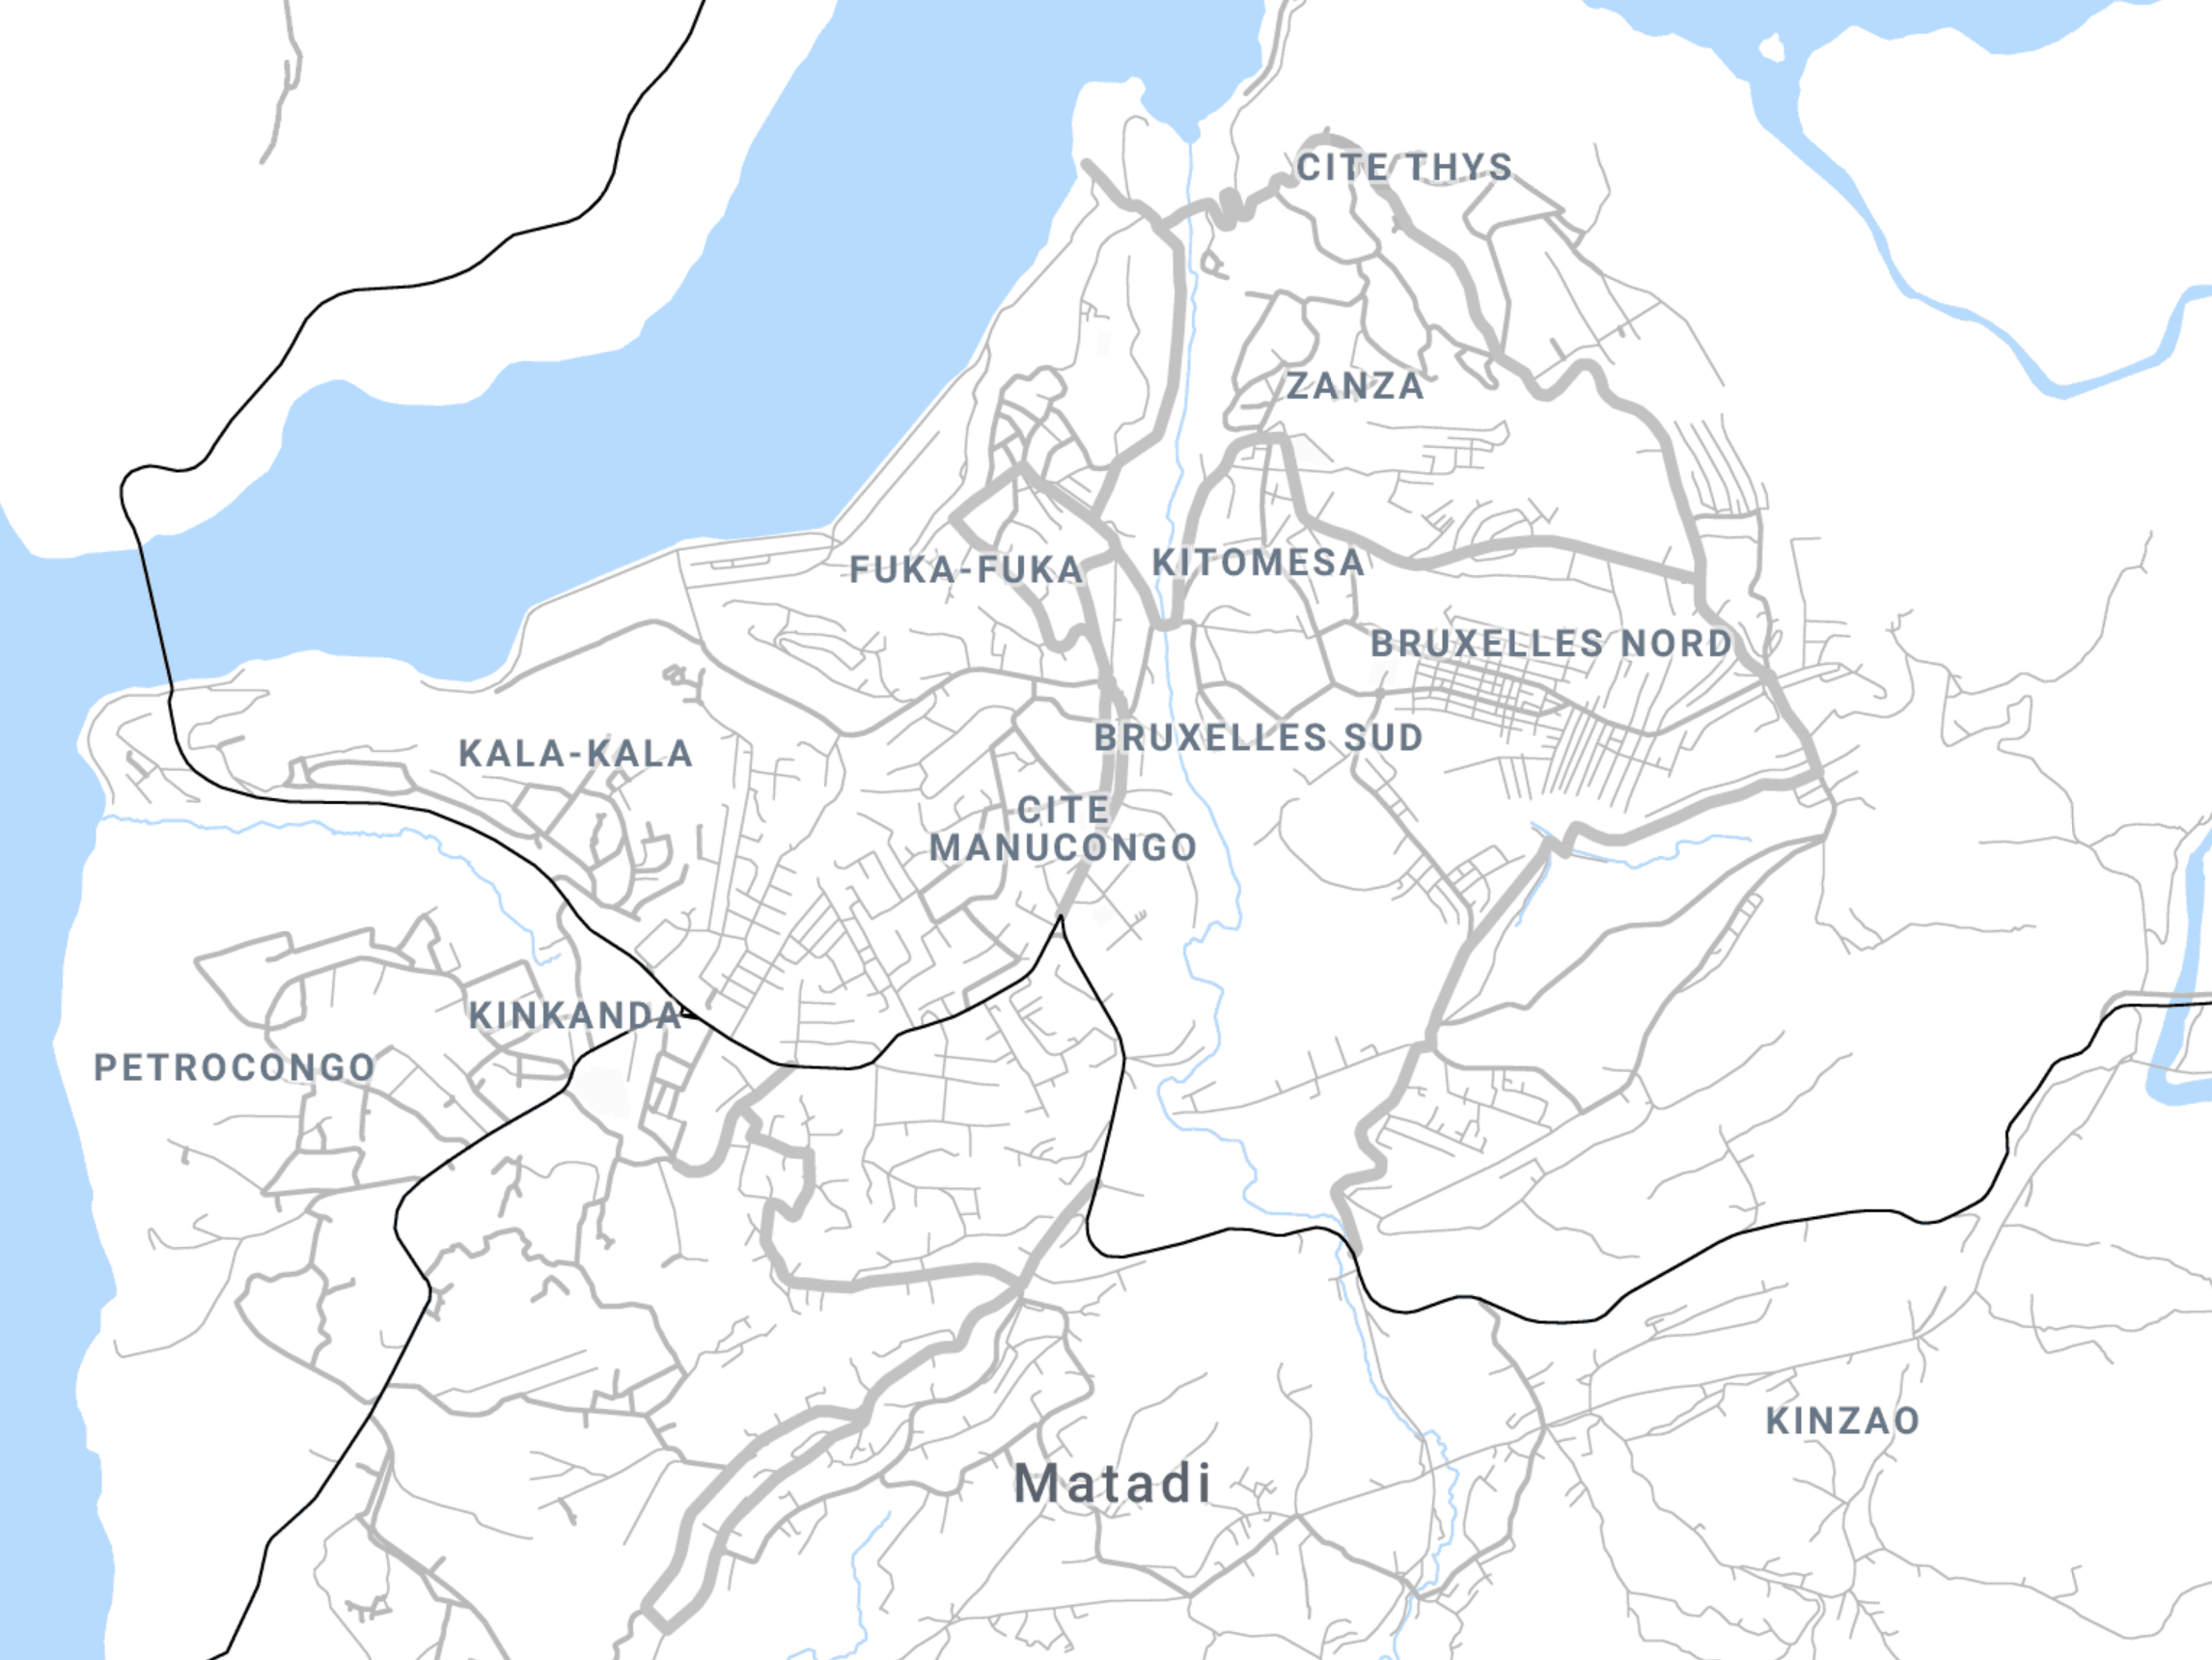
\includegraphics[width=0.8\textwidth]{Figures/matadi.png}
    \caption{Map of Matadi, Democratic Republic of Congo.}
    \label{map:matadi}
\end{figure}

There is insufficient data about the outbreak and specific populations in areas of Matadi, so some assumptions needed to be made. The total population of Matadi in 2005 was 204\,000 \cite{alberti2010reactive}, and a presumed 46\% of this population was under the age of 15 \cite{demographic_dividend}. The total population used for the simulation is thus 93\,840, split between different locations in the city. The network points used for the simulation correspond to the areas labelled on the map in Figure \ref{map:matadi}. The vaccination rate prior to intervention in Matadi was 87.5\% \cite{alberti2010reactive}, and so, the majority of the population was immune to measles. The input data used for the simulation is contained in Table \ref{tab:matadi_input}, where N represents the number of children under 15 in each location, and S represents the number of susceptible children in each location. Since Matadi is a dense city rather than a rural area, the assumptions on travel speeds for a general network do not necessarily apply to this case. Therefore, travel times between locations by road (as obtained from Google Maps) are also used for input, instead of road distances. 

\begin{table}[ht!]
\centering
\resizebox{\textwidth}{!}{%
\begin{tabular}{|c|ccccccccccc|}
\hline
 & \multicolumn{1}{c|}{Urban} & \multicolumn{1}{c|}{x} & \multicolumn{1}{c|}{y} & \multicolumn{1}{c|}{N} & \multicolumn{1}{c|}{S} & \multicolumn{1}{c|}{E} & \multicolumn{1}{c|}{I} & \multicolumn{1}{c|}{V} & \multicolumn{1}{c|}{R} & \multicolumn{1}{c|}{mapX} & mapY \\ \hline
Petrocongo & 0 & -759.07 & 1746.68 & 2000 & 250 & 0 & 0 & 1750 & 0 & -758 & 1747 \\ \cline{1-1}
Cite Thys & 1 & -755.69 & 1751.36 & 3000 & 375 & 0 & 0 & 2625 & 0 & -755 & 1751 \\ \cline{1-1}
Kinzao & 0 & -760.188 & 1753.05 & 1000 & 125 & 0 & 0 & 875 & 0 & -759 & 1752 \\ \cline{1-1}
Bruxelles Sud & 1 & -757.57 & 1750.45 & 15000 & 1875 & 0 & 0 & 13120 & 0 & -758 & 1750 \\ \cline{1-1}
Kala-Kala & 0 & -757.9 & 1748.11 & 4000 & 500 & 0 & 0 & 3500 & 0 & -758 & 1748 \\ \cline{1-1}
Kinkanda & 1 & -758.94 & 1747.98 & 9000 & 1125 & 0 & 0 & 7875 & 0 & -759 & 1748 \\ \cline{1-1}
Cite Manucongo & 1 & -758.004 & 1749.54 & 15000 & 1875 & 0 & 2 & 13120 & 0 & -758 & 1750 \\ \cline{1-1}
Bruxelles Nord & 1 & -757.25 & 1752.478 & 15000 & 1875 & 0 & 0 & 13125 & 0 & -757 & 1752 \\ \cline{1-1}
Fuka-Fuka & 1 & -757.25 & 1749.54 & 10840 & 1355 & 0 & 0 & 9485 & 0 & -757 & 1750 \\ \cline{1-1}
Kitomesa & 1 & -756.86 & 1750.58 & 15000 & 1875 & 0 & 0 & 13125 & 0 & -757 & 1751 \\ \cline{1-1}
Zanza & 1 & -756.47 & 1751.23 & 4000 & 500 & 0 & 0 & 3500 & 0 & -756 & 1751 \\ \hline
\end{tabular}%
}
\caption{Matadi network location details, including populations and coordinates.}
\label{tab:matadi_input}
\end{table}

Since the Matadi network is much smaller and more densely populated than the general network of 160km diameter considered for this project, the frequency of migration needed to be adjusted. Therefore, after adjusting parameters, the amount of migration between any two locations $i$ and $j$ in the Matadi network is $$m_{i,j} = 2 \frac{\sqrt[4]{N_{i} N_{j}}}{\Delta_{i,j}^{2}}.$$ This adjustment reduces the impact that populations have on migration (by setting the exponent of the denominator to $\frac{1}{4}$ instead of $\frac{1}{2})$, to produce more feasible levels of migration for the densely populated network. 

For the simulation of the Matadi outbreak, the death rate is set to 2\% (instead of 10\%), the intervention length to two weeks (instead of four), the number of teams to 18 (instead of 15), and the $R_{0}$ value to 14 (instead of 15). Further, the proportion of a population to be infected before epidemic detection is set to 0.005\% (instead of 0.05\%). All of these parameters are adjusted to mimic the actual results of the outbreak. Figure \ref{res:matadi_valid} shows a comparison of the actual weekly reported measles cases with the average results from over 1000 simulations using this parameter set. The data on the weekly reported measles cases is obtained from Alberti et. al \cite{alberti2010reactive}. The performance of the simulation is easily adjusted according to parameter selection. The team allocation strategy used is population (N), and the vaccine delivery allocation strategy is the number of infectious individuals (I). It is assumed that deliveries are performed by vehicle, since UAVs were not being used for humanitarian aid at the time of the outbreak.

\begin{figure}[ht!]{\textwidth}
    \centering
    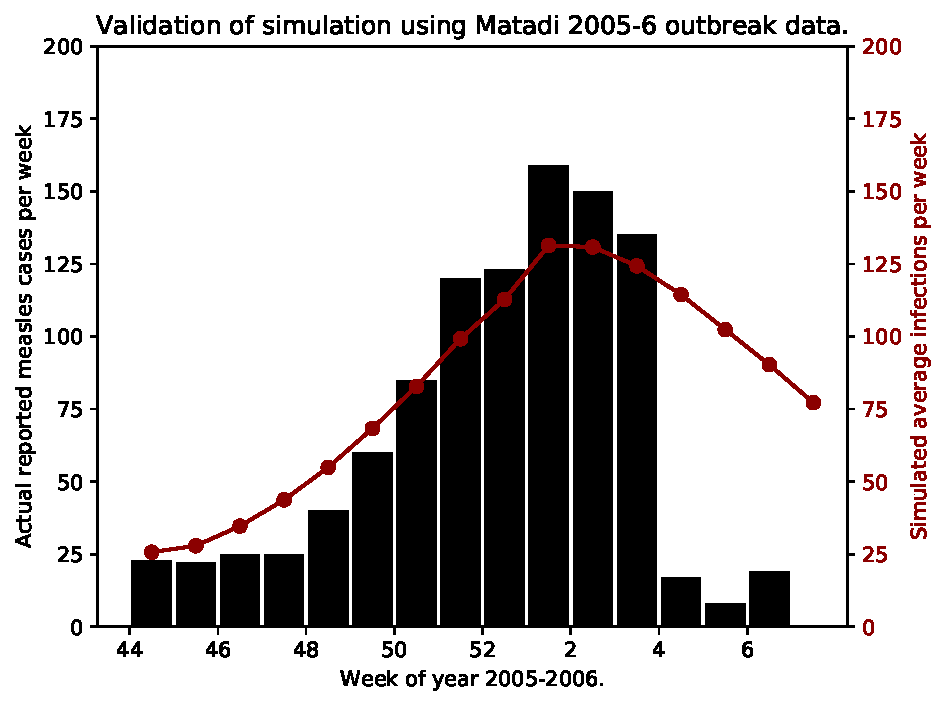
\includegraphics[width=\textwidth, trim={0 0 0 0.67cm},clip]{Matadi_updated.pdf}
    \caption{Comparison of historical measles outbreak results in Matadi with average simulated results.}
    \label{res:matadi_valid}
\end{figure}

The results of the simulation on the Matadi network are similar to the actual outbreak -- an average of 2.26 deaths occurred in simulations (with standard deviation of 1.88), and 9\,315 vaccinations were performed on average (or 71\,884, if previously-vaccinated individuals are re-vaccinated, as was likely the case in the actual intervention). The average progression of the epidemic, as shown in Figure \ref{res:matadi_valid}, is close to the reported outbreak results. It is, however, clear that the intervention in the actual outbreak was significantly more effective and faster than the simulated intervention -- perhaps indicating that teams were able to vaccinate more people daily than in simulations. Using a variable turnout dependant upon the progression of the epidemic, instead of the constant turnout used, would likely produce more accurate results. There are reports of extremely high turnout at vaccination sites for the reported intervention \cite{msf_2006}, and the reported number of weekly infections is not necessarily the same as the number of currently-infected individuals. Thus, these factors can possibly account for the rapid decline in the number of reported infections seen in Figure \ref{res:matadi_valid}, when compared to simulations.

The results of this test for validity of the simulation model indicate that the model is indeed valid, since it can reproduce historical epidemics fairly accurately. The model would likely be even more accurate if more detailed data could be used as input, and parameters could be more finely tuned. Furthermore, the model is consistent -- the standard deviation of results is relatively low. It can therefore be concluded that the model is valid and results produced are likely to be reliable.

\chapter{Results}
A case study of a fabricated measles outbreak is discussed in \S \ref{sec:res_caseS}, which is used for the generation of the results in this chapter. The base set of parameters used is discussed in \S \ref{sec:res_baseCase}, along with a presentation of the base case of the epidemic model using those parameters. Results regarding the resource allocation models and delivery methods tested are discussed in \S \ref{sec:res_resAllocModel} and \S \ref{sec:res_delMethRes}, respectively. Sensitivity analysis is performed on the parameters outside of the control of intervention decision-makers, in \S \ref{sec:res_sensAn}. The chapter is concluded with an evaluation of scenario tests and factors which are under the control of intervention decision-makers, in \S \ref{sec:res_scenTests}.

\section{Case study}
\label{sec:res_caseS}
In order to obtain results, compare resource allocation strategies and evaluate UAV delivery as an alternative to vehicle vaccine delivery, a fabricated measles outbreak is simulated in Likasi and surrounds, in the Democratic Republic of Congo (DRC). Likasi is a large city of over 400\,000 people, with a number of smaller towns and villages nearby -- some of which are only accessible by unmarked paths and roads, which are likely impassable at times. In this case, the number of locations is $n = 12.$ A map of the area is illustrated in Figure \ref{map:likasi}.

\begin{figure}[ht!]{\textwidth}
    \centering
    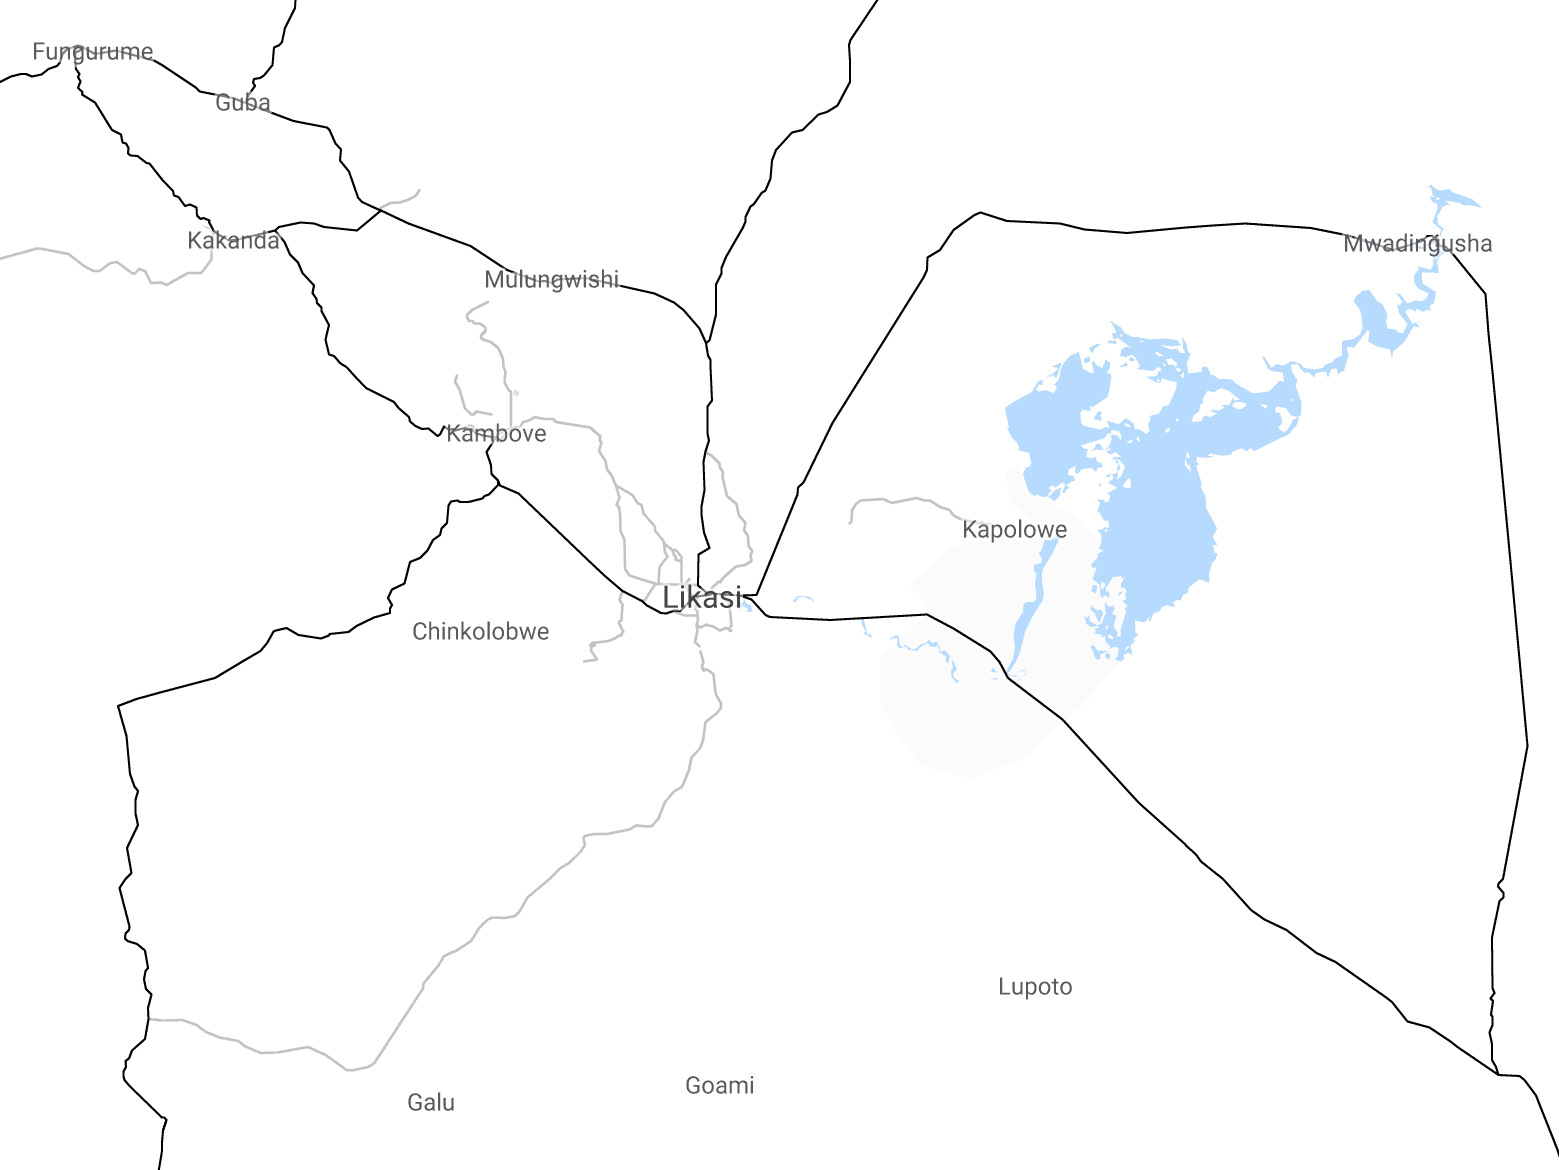
\includegraphics[width=0.8\textwidth]{likasi.png}
    \caption{Map of Likasi and surrounds, Democratic Republic of Congo}
    \label{map:likasi}
\end{figure}

Road distances between locations were procured from Google Maps, and Cartesian coordinates of the locations were estimated. Table \ref{tab:roadDistances} contains the road distances found. If there is no direct road between locations $i$ and $j$, the distance is marked as unavailable. If there is a direct road, the distance is given in kilometres.

\begin{table}[h]
\centering
\resizebox{\textwidth}{!}{%
\begin{tabular}{|c|cccccccccccc|}
\hline
 & \multicolumn{1}{c|}{Fungurume} & \multicolumn{1}{c|}{Guba} & \multicolumn{1}{c|}{Kakanda} & \multicolumn{1}{c|}{Mul...shi} & \multicolumn{1}{c|}{Kambove} & \multicolumn{1}{c|}{Chi...bwe} & \multicolumn{1}{c|}{Likasi} & \multicolumn{1}{c|}{Kapolowe} & \multicolumn{1}{c|}{Mwa...sha} & \multicolumn{1}{c|}{Galu} & \multicolumn{1}{c|}{Goami} & Lupoto \\ \hline
Fungurume & 0 & 12 & 24 & - & - & - & - & - & - & - & - & - \\ \cline{1-1}
Guba & 12 & 0 & 27 & 28 & - & - & - & - & - & - & - & - \\ \cline{1-1}
Kakanda & 24 & 27 & 0 & 25 & 29 & - & - & - & - & - & - & - \\ \cline{1-1}
Mulungwishi & - & 28 & 25 & 0 & - & - & 34 & - & - & - & - & - \\ \cline{1-1}
Kambove & - & - & - & 29 & 0 & - & 25 & - & - & - & - & - \\ \cline{1-1}
Chinkolobwe & - & - & - & - & - & 0 & - & - & - & - & - & - \\ \cline{1-1}
Likasi & - & - & - & 34 & 25 & - & 0 & 32 & 73 & 50 & - & - \\ \cline{1-1}
Kapolowe & - & - & - & - & - & - & 32 & 0 & 70 & - & - & - \\ \cline{1-1}
Mwandingusha & - & - & - & - & - & - & 73 & 70 & 0 & - & - & - \\ \cline{1-1}
Galu & - & - & - & - & - & - & 50 & - & - & 0 & - & - \\ \cline{1-1}
Goami & - & - & - & - & - & - & - & - & - & - & 0 & - \\ \cline{1-1}
Lupoto & - & - & - & - & - & - & - & - & - & - & - & 0 \\ \hline
\end{tabular}
}
\caption{Distances by road between locations in the network (in kilometres).}
\label{tab:roadDistances}
\end{table}

The population values used are contained in Table \ref{tab:podDetails}, split into categories for vaccinated (V) and susceptible (S), as well as exposed (E), infected (I) and recovered (R). Scaled euclidean coordinates of the locations (x,y) are included in Table \ref{tab:podDetails}, as well as a column indicating whether the location is urban or not.  In the table, the columns \textit{mapX} and \textit{mapY} represent (x,y) coordinates for plotting the location's details on the map, and are not used for calculations. Note that all previously-vaccinated individuals are placed in the V category and thus, vaccination is targeted to individuals with no history of previous vaccination. 

\begin{table}[h]
\centering
\resizebox{\textwidth}{!}{%
\begin{tabular}{|c|ccccccccccc|}
\hline
 & \multicolumn{1}{c|}{Urban} & \multicolumn{1}{c|}{x} & \multicolumn{1}{c|}{y} & \multicolumn{1}{c|}{N} & \multicolumn{1}{c|}{S} & \multicolumn{1}{c|}{E} & \multicolumn{1}{c|}{I} & \multicolumn{1}{c|}{R} & \multicolumn{1}{c|}{V} & \multicolumn{1}{c|}{mapX} & \multicolumn{1}{c|}{mapY} \\ \hline
Fungurume & 1 & 7.11 & 105.69 & 18400 & 5152 & 0 & 0 & 0 & 13258 & 87 & 35 \\ \cline{1-1}
Guba & 1 & 17.83 & 100.03 & 920 & 258 & 0 & 0 & 0 & 662 & 243 & 87 \\ \cline{1-1}
Kakanda & 1 & 16.54 & 88.54 & 9200 & 2576 & 0 & 0 & 0 & 6624 & 225 & 227 \\ \cline{1-1}
Mulungwishi & 1 & 39.43 & 86.83 & 4600 & 1288 & 0 & 0 & 0 & 3312 & 541 & 265 \\ \cline{1-1}
Kambove & 1 & 36.60 & 75.86 & 17020 & 4766 & 0 & 0 & 0 & 12254 & 483 & 415 \\ \cline{1-1}
Chinkolobwe & 0 & 33.69 & 62.14 & 184 & 52 & 0 & 0 & 0 & 132 & 469 & 611 \\ \cline{1-1}
Likasi & 1 & 48.60 & 64.71 & 207000 & 57960 & 0 & 5 & 0 & 149035 & 703 & 579 \\ \cline{1-1}
Kapolowe & 1 & 72.69 & 69.17 & 6440 & 1803 & 0 & 0 & 0 & 4637 & 1007 & 515 \\ \cline{1-1}
Mwandingusha & 0 & 106.46 & 90.00 & 1840 & 515 & 0 & 0 & 0 & 1325 & 1413 & 231 \\ \cline{1-1}
Galu & 0 & 33.60 & 26.40 & 276 & 77 & 0 & 0 & 0 & 199 & 433 & 1081 \\ \cline{1-1}
Goami & 0 & 53.74 & 27.86 & 120 & 34 & 0 & 0 & 0 & 86 & 715 & 1065 \\ \cline{1-1}
Lupoto & 0 & 75.00 & 36.43 & 230 & 64 & 0 & 0 & 0 & 156 & 1031 & 961 \\ \hline
\end{tabular}%
}
\caption{Network location details, including populations and coordinates.}
\label{tab:podDetails}
\end{table}

Population values for the network locations were estimated using census data, and satellite imagery when data was unavailable. Measles vaccinations are usually performed on children aged 9 months to 15 years, as early as possible \cite{danet_fermon_2013}. Since 46\% of the population in the DRC are below the age of 15 \cite{demographic_dividend}, and the measles vaccination rate in the country is most recently estimated to be 72\% \cite{who_2018_coverage}, the number of susceptible people used as input for the model is significantly less than the total population.

\section{Epidemic model results}
\label{sec:res_baseCase}
Since the simulation has many components which vary randomly , repeated simulations are required to nullify any random biases in the results. This repeated simulation is performed according to the process described in \S \ref{sec:meth_sim_res}, with a base set of initial parameter values listed in Table \ref{tab:res_baseParams}.

\begin{table}[ht!]
\centering
\resizebox{\textwidth}{!}{%
\begin{tabular}{|c|c||c|c|}
\hline
\multicolumn{1}{|c|}{\textbf{Parameter}} & \textbf{Value} & \multicolumn{1}{c|}{\textbf{Parameter}} & \textbf{Value}  \\ \hline
$\sigma$                         & $\frac{1}{10}$ &    Death Rate                       & 10\%              \\
$\beta$                          & $\frac{15}{8}$ & Work days per week                & 7 days               \\
$\gamma$                    & $\frac{1}{8}$       & Intervention delay      & 15 days         \\
$R_{0}$                         & 15            & Intervention length                     & 28 days \\
$k_{m}$                          & 1              & Primary vehicle capacity         & 1050 vaccines   \\
$\mu$                       & $\frac{0.1}{8}$   & Secondary vehicle capacity      & 200 vaccines        \\
$\lambda_{S}$                  & 0.95           & UAV capacity                    & 60 vaccines      \\
$\lambda_{E}$                   & 0.83           & Average UAV speed               & 100 km/h        \\
$\mathcal{K}$                   & 1             & Combined delivery cutoff time   & 180 minutes   \\
$\mathcal{N}$                   & 15 teams      &  $\psi_{i}$ per fixed-post team  & 450 vaccinations \\   
$\mathcal{H}$                 & 660 minutes    & $\psi_{i}$ per mobile team   & 250 vaccinations     \\
Epidemic detection ratio     & 0.5\%           & Number of vehicles   &  2   \\ \hline
\end{tabular}%
}
\caption{Base set of parameters for simulation.}
\label{tab:res_baseParams}
\end{table}

A base case of the simulation is performed with no vaccine deliveries and epidemic parameters set to the values given in Table \ref{tab:res_baseParams}. 
The progression of the population between the different compartmental model categories is shown in Figure \ref{fig:SEIRnoV}. Most of the population becomes infected with measles and recovers, although there are a significant number of deaths also. Repeating this simulation 500 times gives an average of 6\,504 deaths per epidemic. 

\begin{figure}[ht]{\textwidth}
    \centering
     \subfloat[Epidemic progression without intervention.]{
       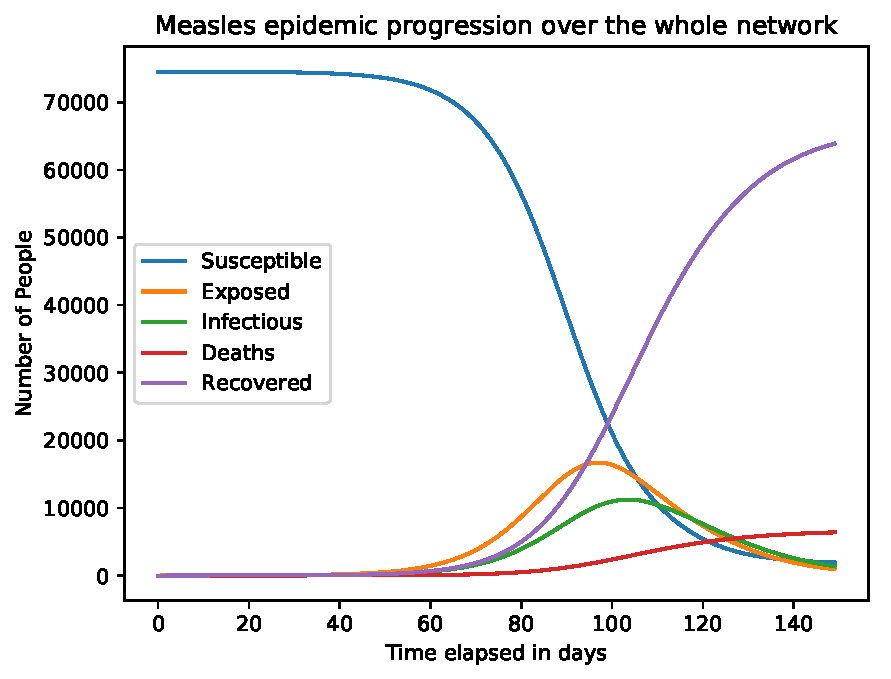
\includegraphics[width=0.48\textwidth, trim={0 0 0 0.7cm}, clip]{Figures/SEIRnoV.pdf}
       \label{fig:SEIRnoV}
     }
     \subfloat[Epidemic progression with intervention.]{
       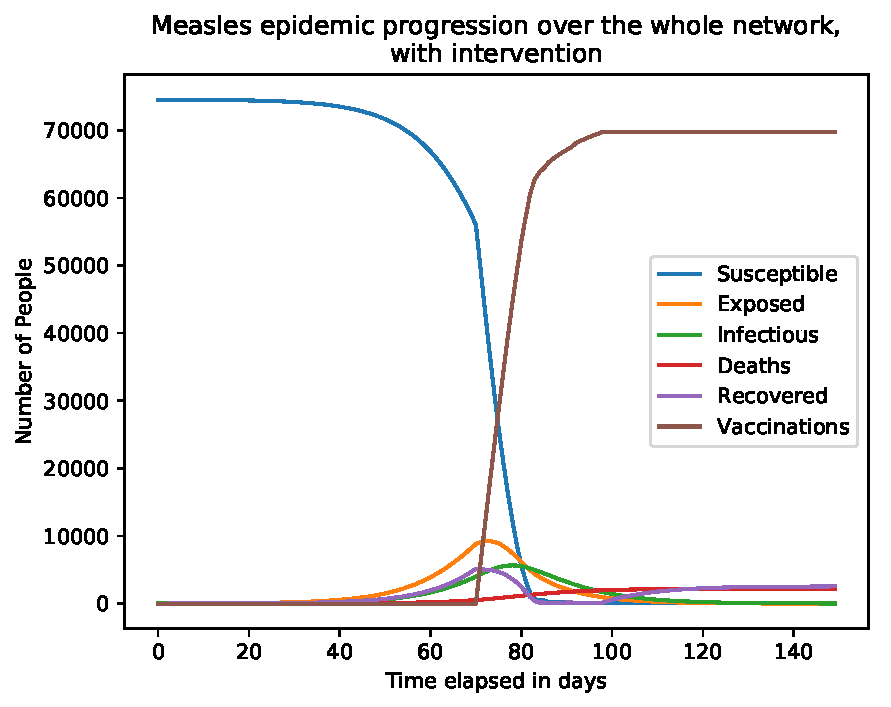
\includegraphics[width=0.48\textwidth, trim={0 0 0 1.2cm}, clip]{Figures/SEIRvehicleD.pdf}
       \label{fig:SEIRvehicleD}
     }
     %add epidemic progression with constant vaccinations intervention
    \caption{Progression of simulated measles epidemic with and without intervention.}
\end{figure}

In Figure \ref{fig:SEIRvehicleD}, the progression of the population between categories, where there is vaccination according to the set of base parameters in Table \ref{tab:res_baseParams}, is shown. Vehicle delivery was used with vaccine allocation strategy $I$ and team allocation strategy $N$. Clearly, vaccination curbs the epidemic's progress considerably -- resulting in an average number of just 2\,212 deaths, at an average total delivery and vaccine cost of \$362\,523.

\section{Resource allocation model results}
\label{sec:res_resAllocModel}
As discussed in detail in \S \ref{sec:vd_strat} and \S \ref{sec:team_strat} respectively, different strategies for vaccine deliveries and team allocations can be employed for an intervention. The team assignment strategies include assigning teams proportionally to I, S, N, or I/N, or to assign them equally across the network, with each location having at least one team. The optimal EPE team assignment strategy can also be used. 

The vaccine delivery strategy determines which locations receive vaccines first, and can be one of I, S, or N, or the optimised EPE delivery strategy. To test which pair of team and vaccine delivery strategies is best, each pair was simulated 500 times, to produce the average results plotted in Figure \ref{fig:res_teamScatter}, and recorded in more detail in Table \ref{tab:vehicle_stratPairs} in Appendix A. For each of the six team strategies, each of the four delivery strategies is simulated and plotted as a point in Figure \ref{fig:res_teamScatter}. The delivery strategy is represented with a letter, and the team strategy by different colours -- so each point is the result of 500 simulations with that strategy pair. As is clear in the figure from the distinct clusters, results are much more dependant upon the team strategy than the delivery strategy. The choice of delivery strategy has very little bearing on the cost or number of deaths, so any delivery strategy used will be successful if the teams are well allocated.

\begin{figure}[ht!]
    \centering
    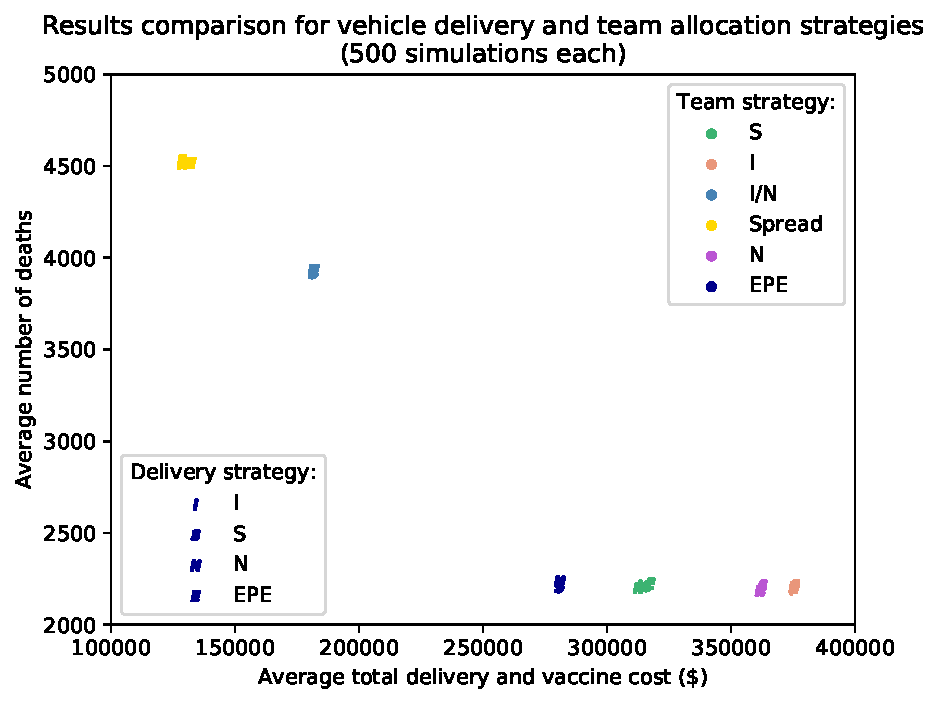
\includegraphics[width=0.9\textwidth, trim={0 0 0 1.15cm}, clip]{teamAssScatter.pdf}
    \caption{Comparison of various vaccine delivery and team assignment strategy pairs, with vehicle delivery for vaccines.}
    \label{fig:res_teamScatter}
\end{figure}

Take note of the four bottom-right clusters in Figure \ref{fig:res_teamScatter}. These four team-allocation strategies (EPE, S, N and I) are clearly the best strategies for minimising deaths, although they incur a higher average total cost. This higher cost is primarily due to a higher number of vaccines administered, causing the reduction in deaths. The strategy pair with the lowest average deaths is (N,N); 2184 deaths at a cost of \$361\,751. The EPE team allocation strategy, paired with the S vaccine delivery strategy, results in an average of 2204 deaths at a cost of \$280\,735. This is a \$35\,196 cost saving from the next cheapest intervention with a similar level of deaths, and a similar number of lives saved to the (N,N) strategy, for a cost of \$81\,016 (22.4\%) less. The EPE team allocation strategy significantly reduces average total delivery and vaccine cost when compared to other strategies with similar numbers of deaths.

For a visual representation of the difference between resource allocation strategy pairs, a selection of pairs were each simulated 500 times, producing the plot shown in Figure \ref{fig:res_avgVaccsPerDay}. This, for each team allocation strategy paired with an appropriate vaccine delivery allocation strategy, shows the average number of vaccinations per day during the simulation. On average, interventions begin between day 60 and 80, and end before day 110. The four best team allocation strategies discussed earlier (EPE, S, N, and I) vaccinate the most people, with the other two strategies performing poorly and not vaccinating enough people to prevent deaths. The cost improvement found for the EPE and S team allocation strategies clearly occurs towards the end of the intervention; while the I and N strategies continue vaccinations, the EPE and S strategies stop. Towards the end of the epidemic, as can be seen in Figure \ref{fig:SEIRvehicleD}, there are essentially no susceptible individuals remaining. Therefore, the I and N strategies waste vaccines on already-recovered and exposed individuals, where those vaccinations actually have no impact. 

The effect of the different resource allocation strategies on a medium-sized town is shown in Figure \ref{fig:res_avpdFungurume}, where the average number of daily vaccinations over time is plotted for each of six strategy pairs, in the town of Fungurume (with population 18\,400). Initially, the epidemic has not yet spread to Fungurume, and only the S, N, and spread strategies perform vaccinations. When the epidemic spreads to Fungurume, there is a large spike in vaccinations for the EPE strategy; since there is now potential for many exposures in Fungurume, many vaccinations are performed. The I and I/N strategies result in vaccinations being performed towards the end of the intervention, only once there are a significant number of infections in Fungurume. 

Clearly, intervention should end once it seems clear that all susceptible people have been vaccinated, in order to reduce cost. This is implemented by the EPE and S strategies well, and therefore they should generally be good strategies for resource allocation decisions.

\begin{figure}[ht!]{\textwidth}
    \centering
     \subfloat[Average number of daily vaccinations over time, for a range of resource allocation strategy pairs (team strategy, followed by delivery strategy).]{
       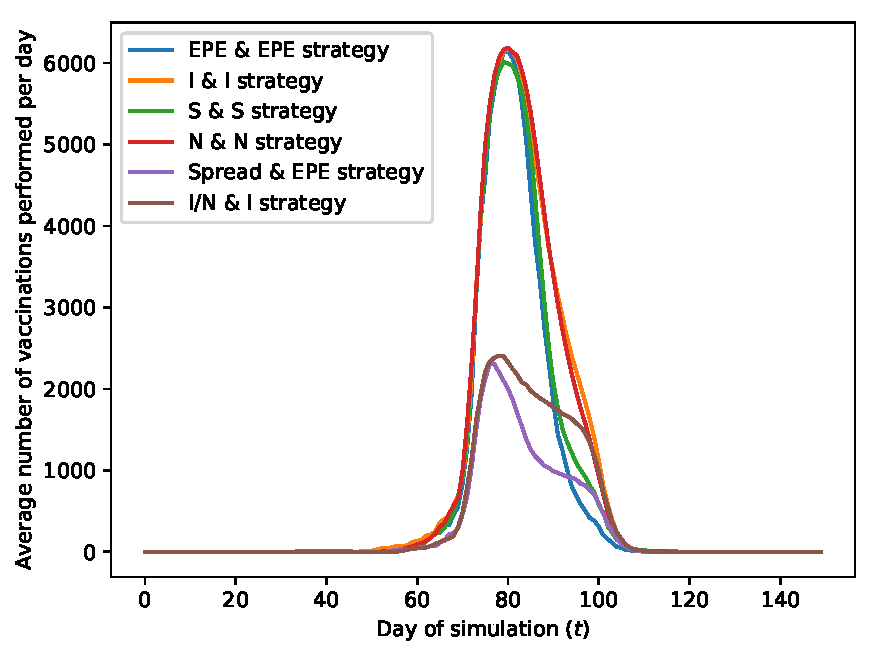
\includegraphics[width=0.47\textwidth]{Figures/vaccCompPlot.pdf}
       \label{fig:res_avgVaccsPerDay}
     }
     \vspace{4}
     \subfloat[Average daily vaccinations over time in Fungurume, for a range of resource allocation strategy pairs.]{
       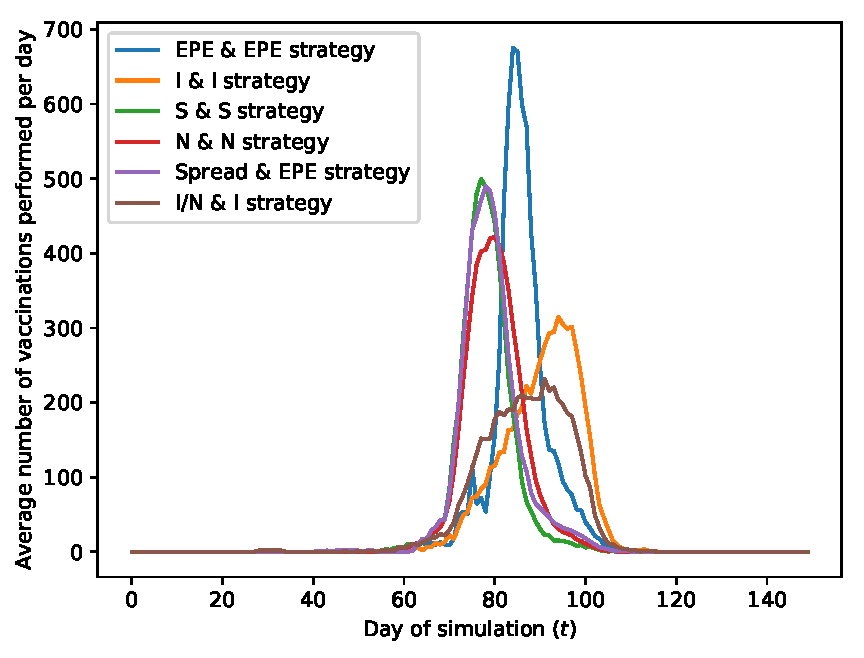
\includegraphics[width=0.47\textwidth]{Figures/vaccCompPlotFungurume.pdf}
       \label{fig:res_avpdFungurume}
     }
    \caption{Depiction of resource allocation strategies over time.}
    \end{figure}

The selection of which locations receive priority for vaccinations also poses an ethical dilemma of sorts. Rural locations generally have worse health infrastructure and consequently, a higher likelihood of measles resulting in death, but urban locations have higher transmission rates. Whether it is best to minimise deaths and exposures across an entire network, or only in cities or rural areas, is a question that cannot necessarily be answered by quantitative methods. To that end, further investigation into resource allocation strategies based on fairness and equity is an interesting topic for future work.

\section{Delivery method results}
\label{sec:res_delMethRes}
A central focus of this project is evaluating the possibility of a UAV delivery network in comparison to a vehicle-based network, or perhaps as an addition to it. Initially, there is assumed to be 2 vehicles available for the vehicle-only network, 2 UAVs for the UAV-only network, and one of each for the combined network. In the combined network, UAVs are used for vehicle deliveries that would take longer than 3 hours.

These three vaccine delivery networks are compared on the basis of cost and deaths, for each pair of team allocation and vaccine delivery strategies. The results of this comparison are plotted in Figure \ref{fig:res_delMethods}, and are listed in more detail in Tables \ref{tab:vehicle_stratPairs}, \ref{tab:UAV_stratPairs}, and \ref{tab:Combined_stratPairs}, of Appendix A.

\begin{figure}[ht!]
    \centering
    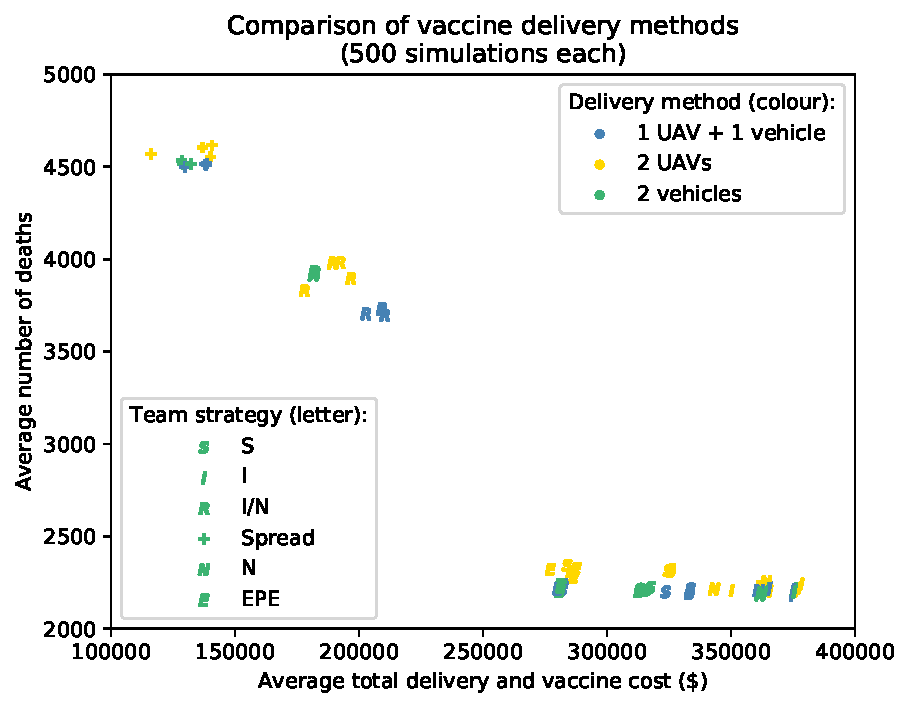
\includegraphics[width=0.9\textwidth, trim={0 0 0 1.15cm}, clip]{Figures/delivMethodScatter.pdf}
    \caption{Comparison of vaccine delivery methods on cost and deaths.}
    \label{fig:res_delMethods}
\end{figure}

Considering Figure \ref{fig:res_delMethods}, the clustering of team strategies is evident as in the vehicle-only network plotted in Figure \ref{fig:res_teamScatter}, although the UAV network's results are more widely spread. All three networks offer similar results to one another, but the UAV network results in marginally more deaths for most strategy pairs. This is due to the small payload of the UAVs, preventing the UAV network from delivering as many vaccines on time as are required. However, having 3 or more UAVs (as shown in Figure \ref{fig:res_numUAVs}) puts the UAV network on par with the vehicle network. 

As can be seen in Figure \ref{fig:res_numVehs}, there is no significant improvement in the delivery network for more than 1 vehicle (because a single vehicle can meet demand for vaccines most of the time). The results of different combinations of vehicles and UAVs are contained in Table \ref{tab:combiSims}, in Appendix A -- they also indicate essentially no change in the delivery network's performance when more vehicles or UAVs are added, for more than 2 UAVs.

\begin{figure}[ht!]{\textwidth}
\centering
 \subfloat[Comparison of number of UAVs on results.]{
   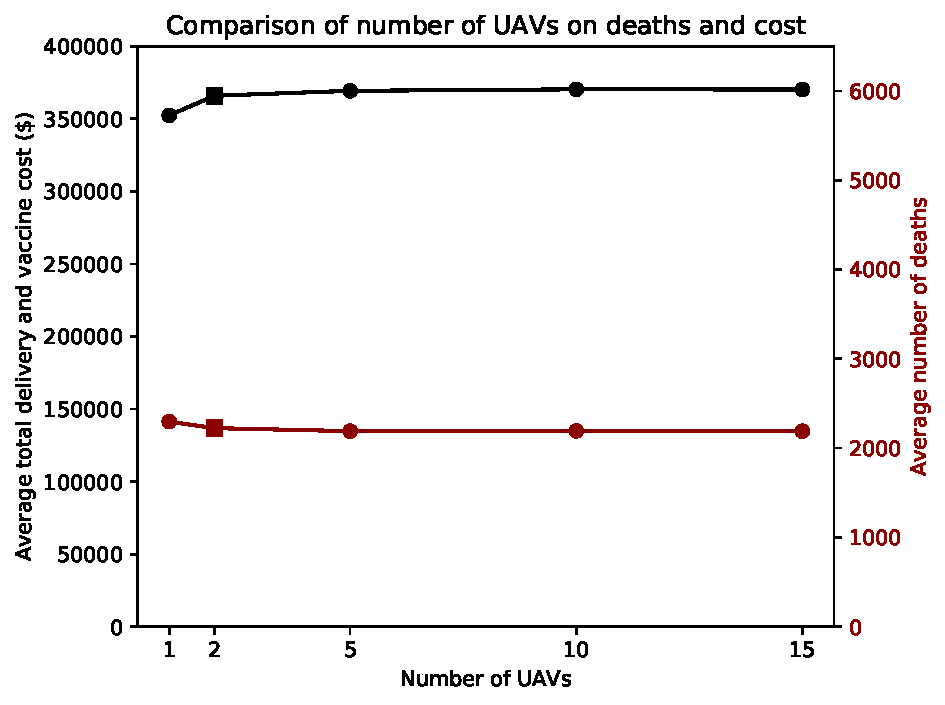
\includegraphics[width=0.48\textwidth, trim={0 0 0 0.67cm}, clip]{Figures/NumberofUAVs.pdf}
   \label{fig:res_numUAVs}
 }
 \subfloat[Comparison of number of vehicles on results.]{
   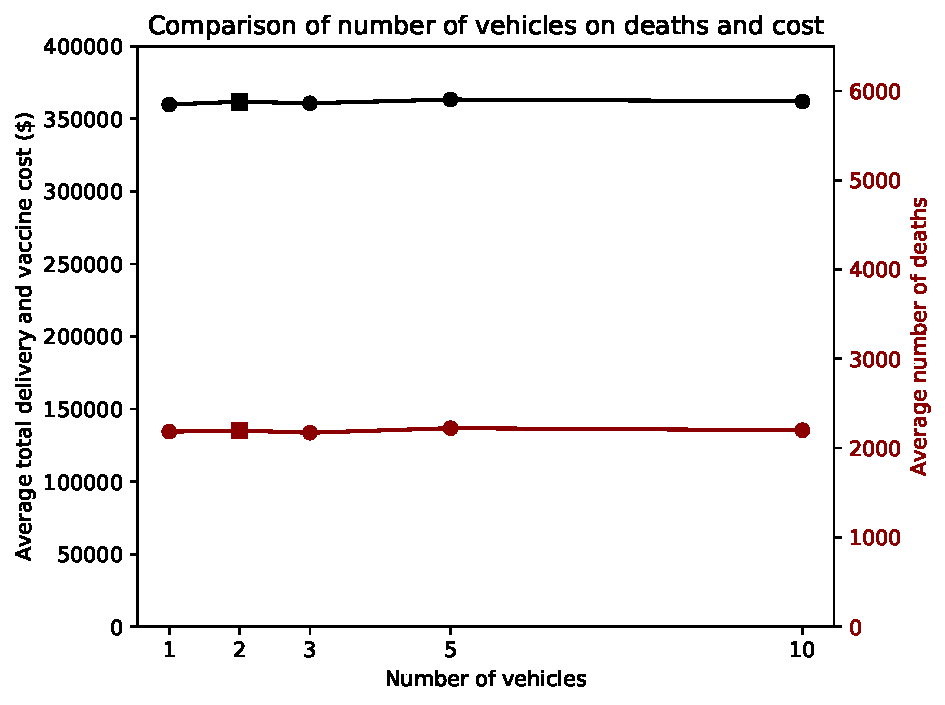
\includegraphics[width=0.48\textwidth, trim={0 0 0 0.67cm}, clip]{Figures/Numberofvehicles.pdf}
   \label{fig:res_numVehs}
 }
\hspace{1pt}
 \subfloat[Effect of differing numbers of impassable roads on results, out of 24 roads in total.]{
   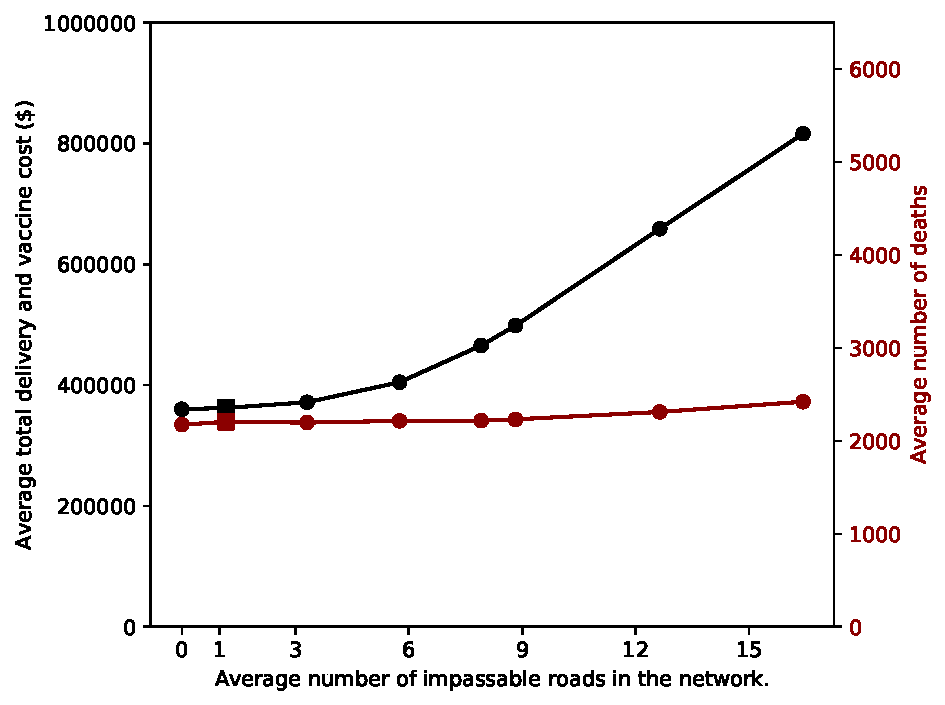
\includegraphics[width=0.48\textwidth]{roads.pdf}
   \label{fig:res_roadProb}
 }

\caption{Effect of differing numbers of UAVs and vehicles, and differing numbers of closed roads, on the performance of vaccine delivery networks.}
\end{figure}

Figure \ref{fig:res_roadProb} shows the impact of worsened road conditions on the average simulated costs and deaths. Clearly, the delivery cost increases exponentially as more roads are set as impassable, while the average number of deaths also rises slightly. This is due to deliveries taking longer, and thus requiring more petrol. With the same resource allocation strategy pair, the average simulated cost of UAV deliveries is \$364\,479 and the average number of deaths is 2\,204. Therefore, if 3 or more roads are closed in the network, UAV delivery (using only 2 UAVs) is cheaper, and results in fewer deaths. Note that there are 24 roads in the network, so this translates to a percentage of 12.5\% of roads; if more than 12.5\% of roads in a network are impassable, UAVs should be a better delivery method than vehicles. However, this is highly dependant on the structure of the network and so, the determination of this `break-even' percentage can be improved by considering a wide range of different networks. This is a good topic for future research; to determine at which point it is better to use UAVs than vehicles, based on a variety of network structures.

As is clear in Figures \ref{fig:res_numUAVs} and \ref{fig:res_roadProb}, UAV delivery with 3 or more UAVs is on par with vehicle delivery networks -- even those on perfect road networks. It can thus be concluded that in locations with poor road infrastructure, UAV delivery is cheaper and more effective than land-based delivery at reducing deaths.

\section{Sensitivity Analysis}
\label{sec:res_sensAn}
Parameters which are mostly out of the control of intervention decision-makers are discussed in this section, to evaluate which parameters have a large impact on average costs and deaths, the output parameters of the simulation.
The approach followed for testing the model output for sensitivity to parameters is varying each parameter individually from its base value, with all other parameters held constant. As each parameter is increased and decreased, changes to the model output parameters (costs and deaths) are observed. The changes in each parameter are according to a range of reasonable values for that parameter. This approach is among those discussed by Pannell \cite{pannell1997sensitivity} for sensitivity analysis. Unless otherwise stated, vehicle deliveries with vaccine allocation strategy $I$ and team allocation strategy $N$ were used in the sensitivity analysis.

\subsubsection{Measles epidemic model parameters}
There are five significant parameters governing the spread of the simulated measles epidemic between individuals, and across locations. The values $\beta, \sigma, \gamma \text{ and } \mu$ determine the movement of individuals between the S and E, E and I, I and R, and I and D classes, respectively. Finally, the fifth parameter $k_{m}$ is a migration frequency multiplier, used in the migration model discussed in \S \ref{sec:meth_migration}. The amount of migration between locations in the model is directly proportional to the value of $k_{m}$, which, in turn, directly affects the speed at which the epidemic spreads between locations.

\begin{figure}[ht!]{\textwidth}
    \centering
     \subfloat[Comparison of durations of exposure.]{
       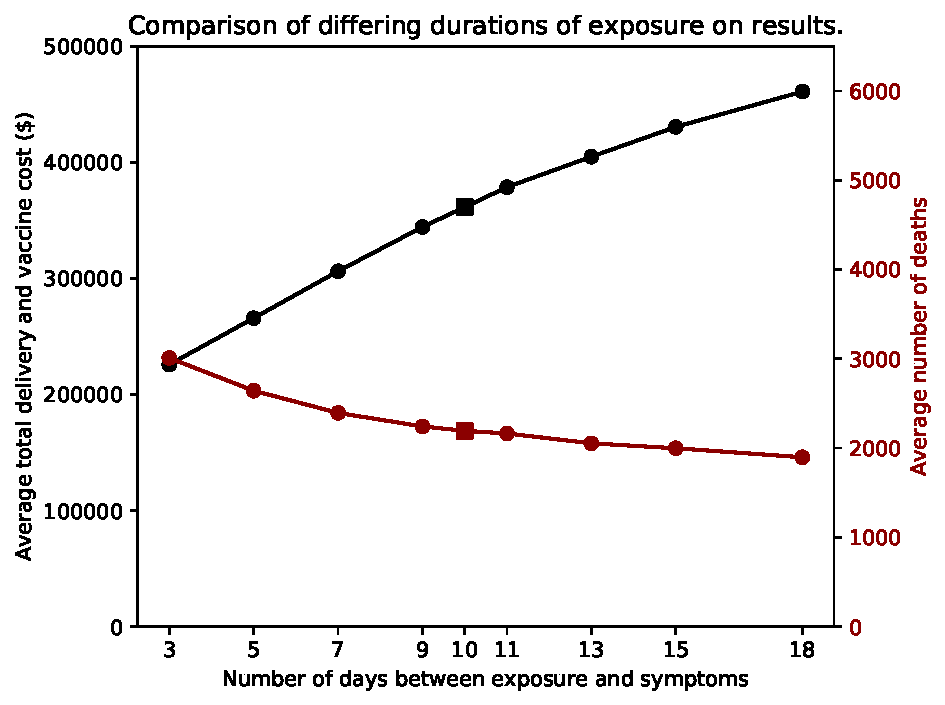
\includegraphics[width=0.48\textwidth, trim={0 0 0 0.67cm}, clip]{Figures/expDays.pdf}
       \label{fig:expDays}
     }
     \subfloat[Comparison of durations of infection.]{
       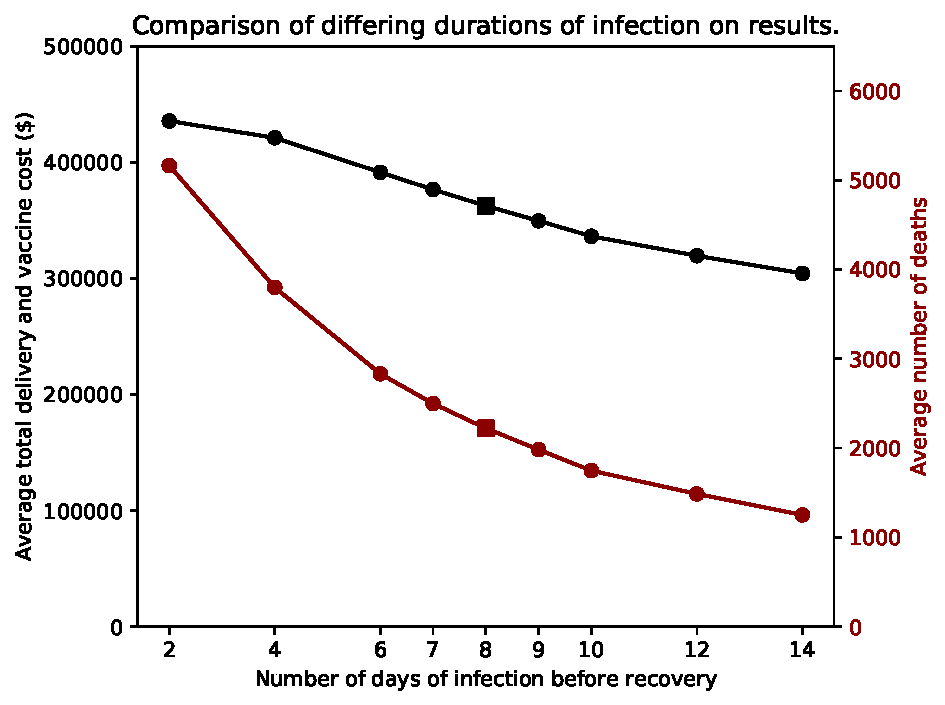
\includegraphics[width=0.48\textwidth, trim={0 0 0 0.67cm}, clip]{Figures/infDays.pdf}
       \label{fig:infDays}
     }
     \vspace{2pt}
     \subfloat[Comparison of death rates.]{
       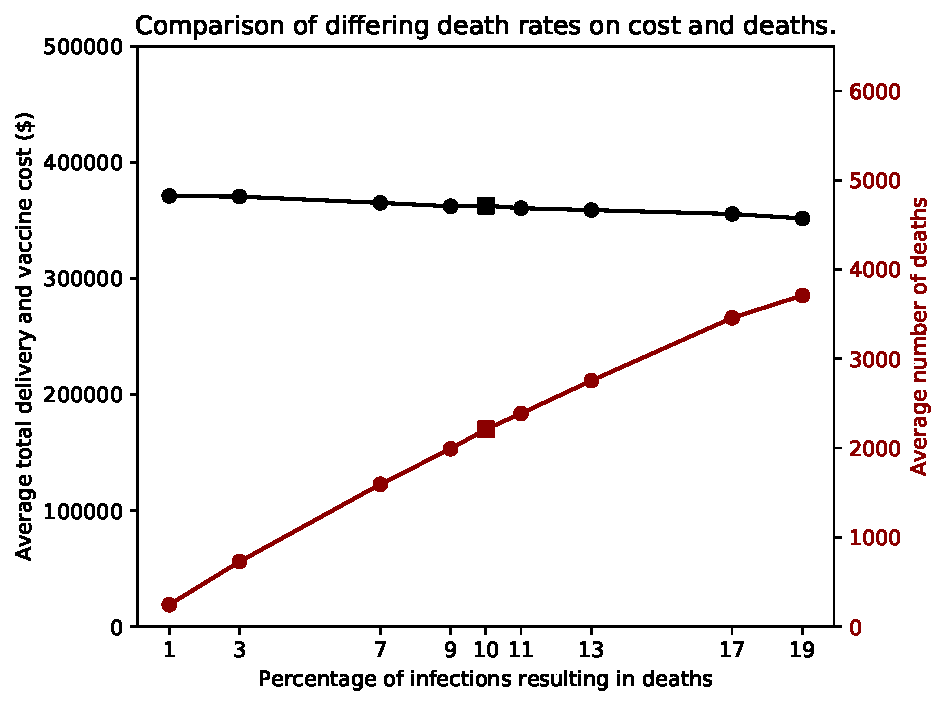
\includegraphics[width=0.48\textwidth, trim={0 0 0 0.67cm}, clip]{Figures/deathRate.pdf}
       \label{fig:deathRate}
     }
     \subfloat[Comparison of $R_{0}$ values.]{
       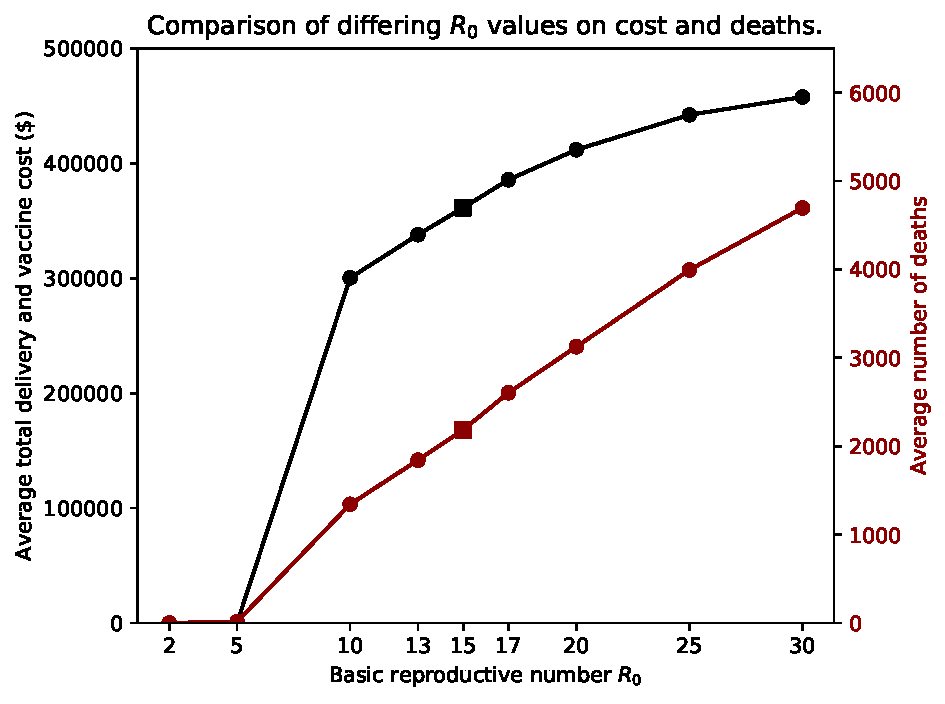
\includegraphics[width=0.48\textwidth, trim={0 0 0 0.67cm}, clip]{Figures/Rzero.pdf}
       \label{fig:Rzero}
     }
\caption{Effects of differing values for epidemic parameters on results.}
\end{figure}

The base values for the aforementioned parameters are discussed below:
\begin{itemize}
    \item $\sigma$ -- Reciprocal of the number of days in the E class between exposure and onset of symptoms. This is more intuitively understood as the proportion of people in the E class moving to the I class, daily. A base value of $\sigma = \frac{1}{10}$ is used, since infection usually follows 10 days after exposure \cite{who_2019}. The number of deaths and the average cost for differing durations of exposure are plotted in Figure \ref{fig:expDays}. As the number of days between exposure and onset of symptoms lengthens, the number of deaths decreases, while cost increases. This is because the epidemic would spread more slowly, allowing more vaccinations to be made before individuals become exposed -- resulting in the increased cost. Note that the cost appears to be more sensitive to changes in this parameter than the number of deaths, although even small increases in the number of deaths may be considered as significant, depending on the decision-maker.
    \item $\gamma$ -- Reciprocal of the number of days of symptoms and contagiousness in the I class. This value corresponds to the proportion of people in the I class moving to the R class daily, and a base value of $\gamma = \frac{1}{8}$ is used -- because infection usually lasts 8 days \cite{who_2019}. As may be seen in Figure \ref{fig:infDays}, if the duration of infection is longer, the number of deaths decreases. A longer duration results in a smaller value for $\gamma$, which in turn results in a smaller value of $\beta$, and the epidemic spreads more slowly.
    \item $\beta$ -- Proportion of the number of people in the S class moving to the E class daily. Note that $\beta = R_{0} \times \gamma$. The value of the basic reproductive number $R_{0}$ is cited much more often than the value of $\beta$, and thus, $\beta$ is calculated in terms of $R_{0}.$ In these simulations, $R_{0}$ is set to 15, meaning that an average of 15 total measles cases are caused by each infectious individual \cite{guerra2017basic}. Any increases in this $R_{0}$ value cause proportional increases in the number of deaths and cost; when the epidemic spreads faster, there is less time for vaccinations to occur. The model is very sensitive to changes in $R_{0}$. Note that for $R_{0}$ values of 5 and below, due to the rounding up and down of values and the small number of index cases, the epidemic usually dies out prematurely. Using continuous values instead of discrete would likely result in more accurate results for this parameter.
    \item $\mu$ -- Daily proportion of infected individuals that die. In literature the total proportion of deaths to infections is often given, so this total proportion is divided by the number of days of infection to get a daily value. Hence, $\mu = \texttt{Death Rate} \times \gamma$, with \texttt{Death Rate} set to 0.1 \cite{moss2007measles}. As expected, when \texttt{Death Rate} is increased, there is an almost exact proportional increase in the number of deaths, which can be seen in Figure \ref{fig:deathRate}. For obvious reasons, the number of deaths is more sensitive to changes in this parameter than the total cost, although cost decreases slightly as the death rate increases, due to the lower number of vaccinations which can occur when more people die.
    
    \begin{figure}[]
    \centering
    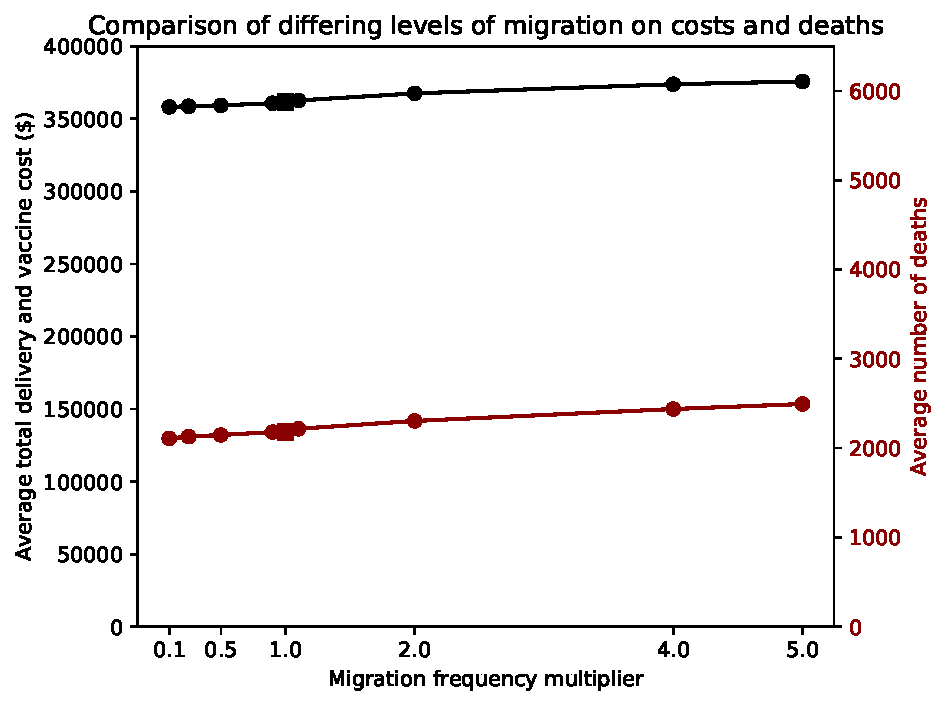
\includegraphics[width=0.5\textwidth, trim={0 0 0 0.67cm}, clip]{Figures/migrationFreq.pdf}
    \caption{Effect of differing levels of migration on results.}
    \label{fig:migrationFreq}
    \end{figure}
    
    \item $k_{m}$ -- Migration frequency multiplier. This is initially set to 1, so that there is no added migration to the basic gravity model of \S \ref{sec:meth_migration}. The amount of migration between locations in the network is directly proportional to this parameter value. The average results of the simulation are plotted in Figure \ref{fig:migrationFreq}, and it is evident in the figure that the model is not sensitive to changes in the amount of migration. As the amount of migration increases, the number of deaths also increase slightly -- because the epidemic spreads across the network faster. Having a high migration multiplier of 5 results in a 14.1\% increase in the number of deaths. Therefore, discouraging movement of individuals between locations during an outbreak can help to curb the spread of it, but is not very effective.
\end{itemize}

Additionally, the number of vaccinations which can occur in a network can be limited by the turnout of people for vaccinations. In urban areas where fixed-post teams are located, the turnout is assumed to be normally distributed with a mean of 900 and a variance of $\frac{900}{5}$. In rural areas, it is assumed to be normally distributed with a mean of 450 and a variance of $\frac{450}{5}$. These values correspond to those in \S \ref{meth:MeaslesCompa}. Varying each across a range of feasible values results in the points plotted in Figures \ref{fig:urbTnt} and \ref{fig:rurTnt}. In both cases, the sensitivity of the number of deaths to turnout is essentially negligible; the number of teams at a location is usually the limiting factor on vaccinations, rather than turnout. However, if turnout were to decrease even further towards the extreme value of zero, it is probable that the model results would become more sensitive to changes in turnout. If turnout was modelled such that it depended upon the progression of the epidemic, results would likely be more sensitive to changes in turnout. 

\begin{figure}[ht!]{\textwidth}
    \centering
     \subfloat[Effect of mean urban turnout on results.]{
       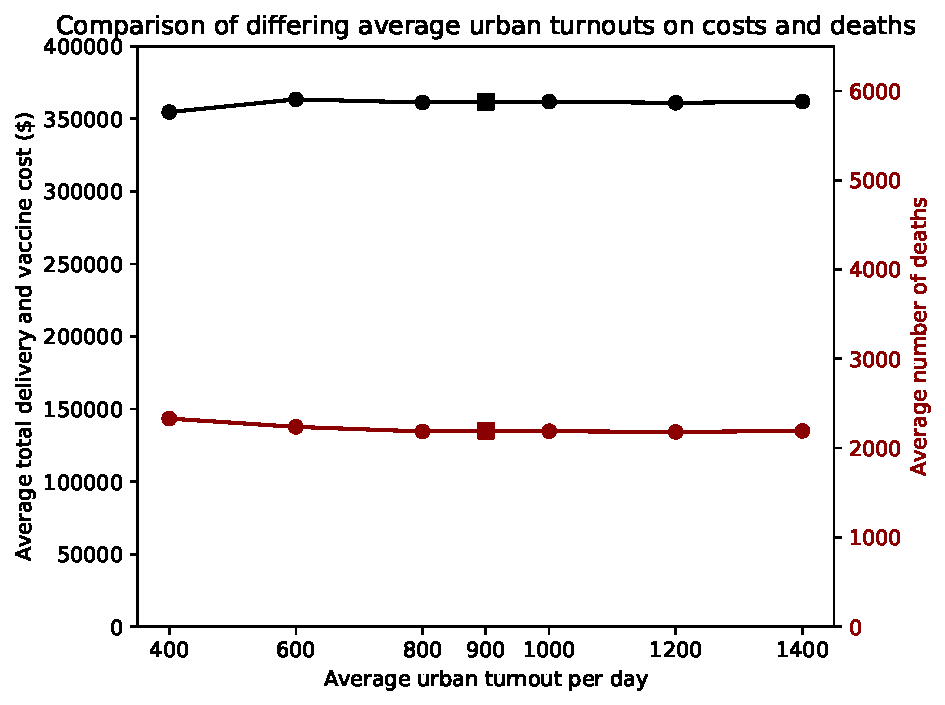
\includegraphics[width=0.48\textwidth, trim={0 0 0 0.67cm}, clip]{Figures/urbanTnt.pdf}
       \label{fig:urbTnt}
     }
     \subfloat[Effect of mean rural turnout on results.]{
       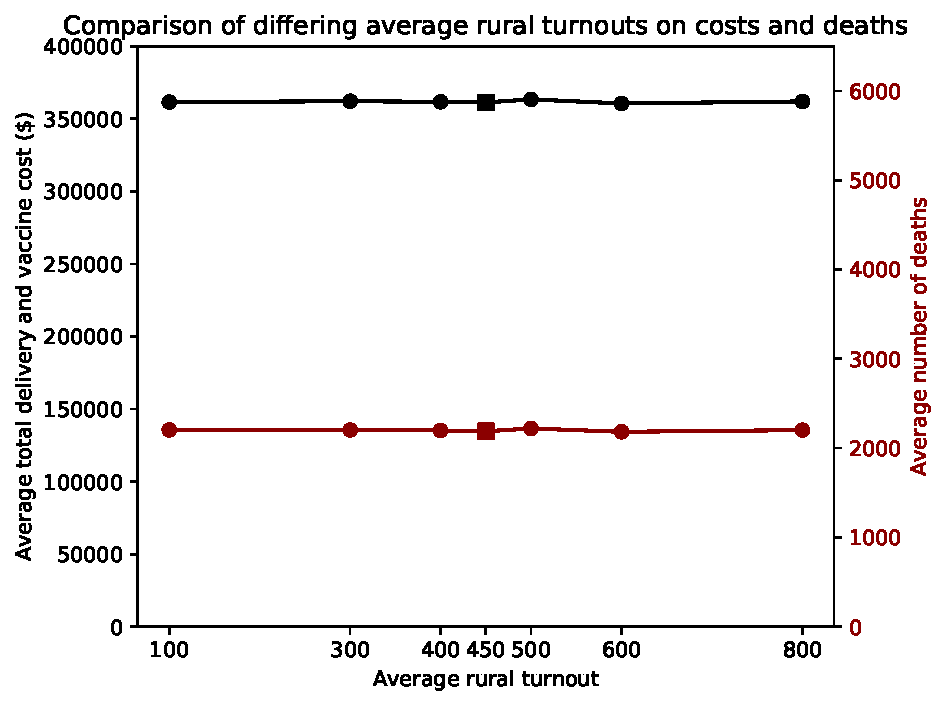
\includegraphics[width=0.48\textwidth, trim={0 0 0 0.67cm}, clip]{Figures/ruralTnt.pdf}
       \label{fig:rurTnt}
     }
\caption{Effect of differing turnout values for rural and urban areas on costs and deaths.}
\end{figure}

\subsubsection{Vaccine-related parameters}
The success rate of the measles vaccine depends on whether the individual receiving the vaccine has been exposed to the measles virus, and whether they have received a dose of the vaccine before. It is assumed that all individuals in the S class have never received a dose of any measles vaccine.
An estimated 2-5\% of first-dose measles vaccinations are unsuccessful \cite{cdc_pinkbook_2018}, so the probability of a vaccinated individual moving from state S to R -- the vaccine success rate $\lambda_{S}$ -- can be reasonably set to $\lambda_{S} = 95\%$. Values ranging between 80\% and 100\% for this success rate were tested, with results plotted in Figure \ref{fig:vaccEfficacy}. It is clear that if the vaccine is more successful or less successful, the only notable difference in results is a slight change in cost, and so the model output is not very sensitive to this parameter.

\begin{figure}[ht!]{\textwidth}
    \centering
     \subfloat[Effect of changes in vaccine efficacy $\lambda_{S}$.]{
       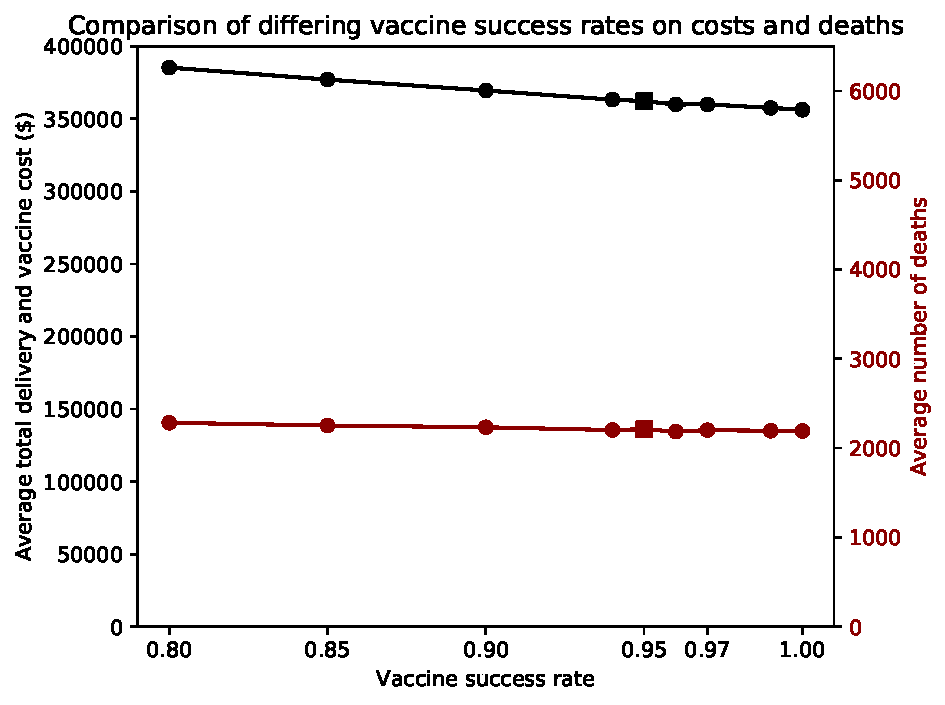
\includegraphics[width=0.48\textwidth, trim={0 0 0 0.67cm}, clip]{Figures/vaccSuccessRate.pdf}
       \label{fig:vaccEfficacy}
     } 
     \subfloat[Effect of changes in prophylaxis efficacy $\lambda_{E}$ .]{
       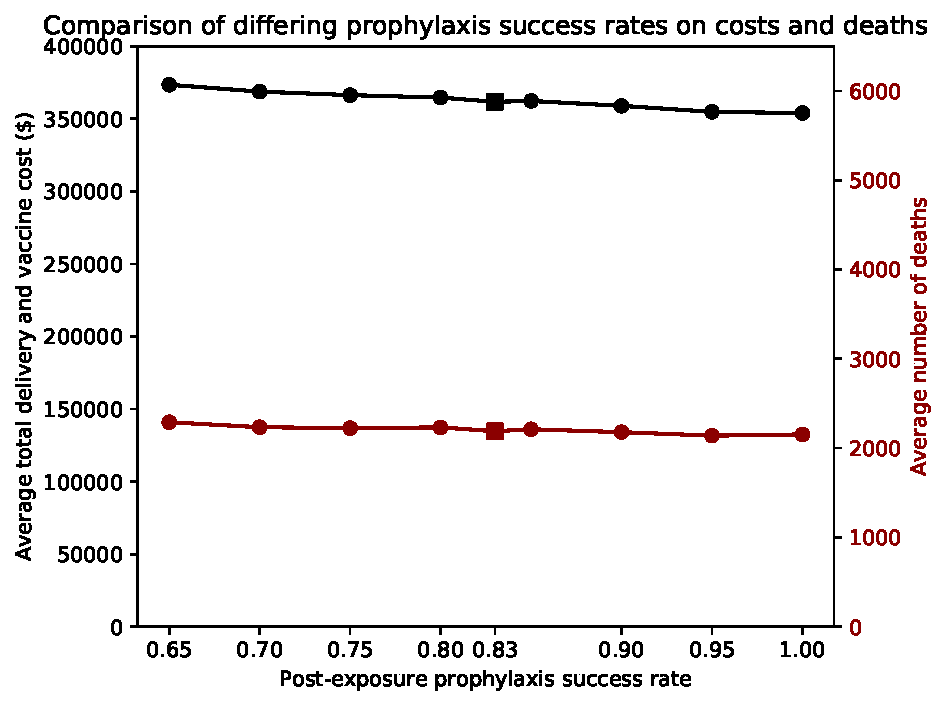
\includegraphics[width=0.48\textwidth, trim={0 0 0 0.67cm}, clip]{Figures/prophEffectiveness.pdf}
       \label{fig:prophEfficacy}
     }
     \vspace{2pt}
     \subfloat[Effect of differing vaccine potency duration values.]{
       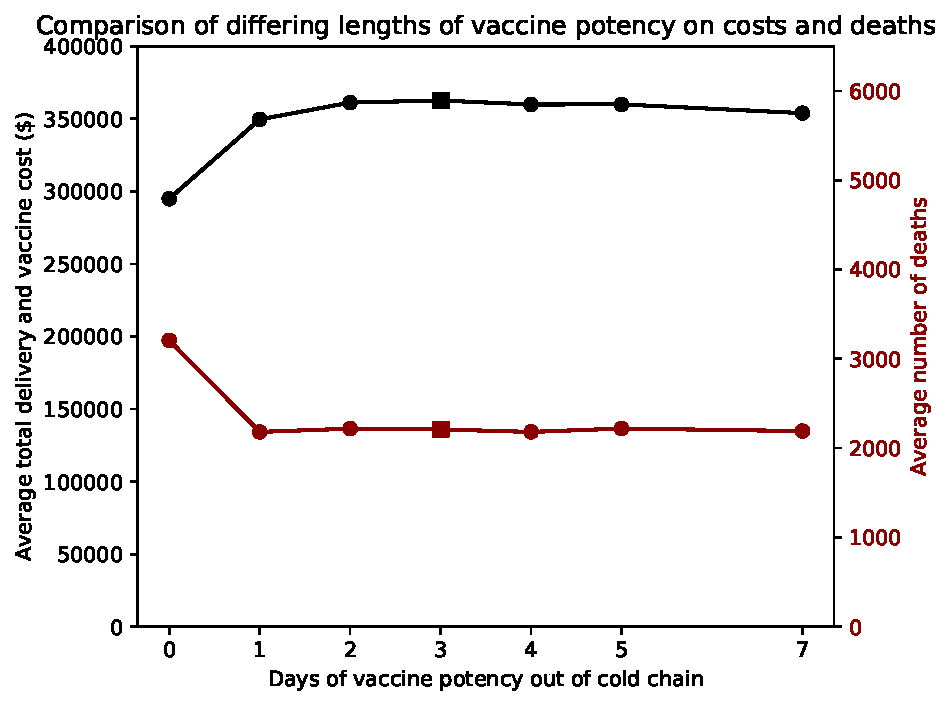
\includegraphics[width=0.48\textwidth, trim={0 0 0 0.67cm}, clip]{Figures/monoDaysPotency.pdf}
       \label{fig:monoDosePotency}
     }
\caption{Sensitivity of vaccine-related parameters.}
\end{figure}

If the individual has only been exposed to the virus for less than 72 hours, they can be given post-exposure prophylaxis. In a 2006 study in Australia, the effectiveness of this prophylaxis for measles cases was found to be 83\% \cite{csiro_2009}. Thus the prophylaxis success rate can be set to $\lambda_{E} = 83\%$. It is thus assumed that 83\% of individuals given prophylaxis are moved directly from the E to the V class, and do not become infectious. As is seen in Figure \ref{fig:prophEfficacy}, values ranging between 65\% and 100\% were tested, with only a slight decrease in deaths and cost as the success rate rises, so the model output is not very sensitive to this parameter.

The measles vaccine can remain at the required potency level outside of the cold chain for 3 days \cite{msf_ectc_2018}. Were this value to change, or even reduce to only a single day, there would be essentially no change in the number of deaths. Figure \ref{fig:monoDosePotency} shows the average number of deaths and total cost for different lengths of potency. There is only an increase in the number of deaths if the vaccine needs to be used on the same day as it is delivered -- and even then, the number of deaths is half of what it would be if there was no intervention. Therefore, transporting the measles vaccine outside of the cold chain is feasible and can considerably reduce cost when compared to the existing cold chain.

\subsubsection{Delivery parameters}
The final set of parameters to be tested for sensitivity are those affecting the delivery network. For the sensitivity analysis pertaining to UAV deliveries, the vaccine allocation strategy $I$ and team allocation strategy $N$ were used, as in the case of vehicle deliveries.

\label{sec:res_del_params}
\begin{itemize}
    \item \textit{The average UAV speed, in kilometres per hour.} An initial value of 100 km/h is used \cite{czerwonka_2018,service_contract_2018, zipline_impact}, and the speed is varied between 20 km/h and 180 km/h to test the impact different speeds have on results. As may be seen in Figure \ref{fig:res_UAVspeed}, results are insensitive to increases in average UAV speed, but sensitive to decreases in average speed below 80km/h. Any slower, and deaths begin to rise as the average speed decreases; because slower UAVs result in teams' requirement for vaccines not being met quickly enough. Therefore, fixed-wing UAVs would be better than the generally slower quadcopters for a network such as this.
    \item \textit{The number of vaccine doses that one UAV can deliver per flight.} A base value of 60 is used, as per the calculations in \S \ref{sec:dro_dels}. Figure \ref{fig:res_UAVcap} shows that as long as UAVs can carry over 30 vaccines, there is no reduction in the average number of deaths. If a UAV could only carry 10 vaccines per flight, the average number of deaths would rise by just under 200. So, with only two UAVs, the UAV-only delivery network is almost able to completely fulfill vaccine demand.
    \item \textit{The number of vaccine doses that vehicles can deliver per route.} Recall that vehicle deliveries are modelled such that routes having any rural areas in them are delivered to by a smaller, secondary vehicle, while all other routes are visited by a primary vehicle. There is initially assumed to be one of each type in the vehicle-only network. Figures \ref{fig:res_primVehCap} and \ref{fig:res_secVehCap} show the results of 500 simulations each for a range of vehicle capacities. Clearly, the vehicle network is able to completely meet vaccine demand, no matter what the capacity of each vehicle is -- provided the capacity is within the tested range.
    \item \textit{The combined network cutoff time.} The combined delivery network, using 1 UAV and 1 vehicle, allows UAVs to deliver to areas that a vehicle would take too long to deliver to. Initially, the maximum allowed vehicle route time is 3 hours. Clearly, other thresholds than 3 hours could also be used with similar success; as can be seen in Figure \ref{fig:res_comboCutoff}, the model output is not very sensitive to changes in this threshold.
\end{itemize}

\begin{figure}[ht!]{\textwidth}
\centering
\subfloat[Effect of differing average UAV speeds on results.]{
   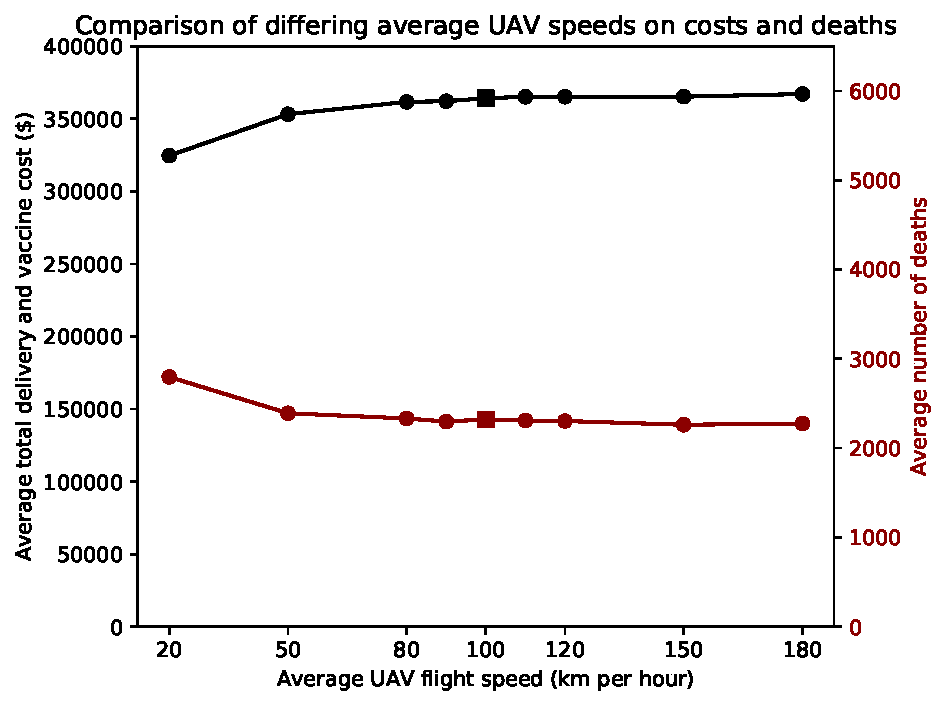
\includegraphics[width=0.47\textwidth, trim={0 0 0 0.67cm}, clip]{Figures/UAVspeed.pdf}
   \label{fig:res_UAVspeed}
 } \hspace{1}
 \subfloat[Effect of differing UAV vaccine capacities on results.]{
   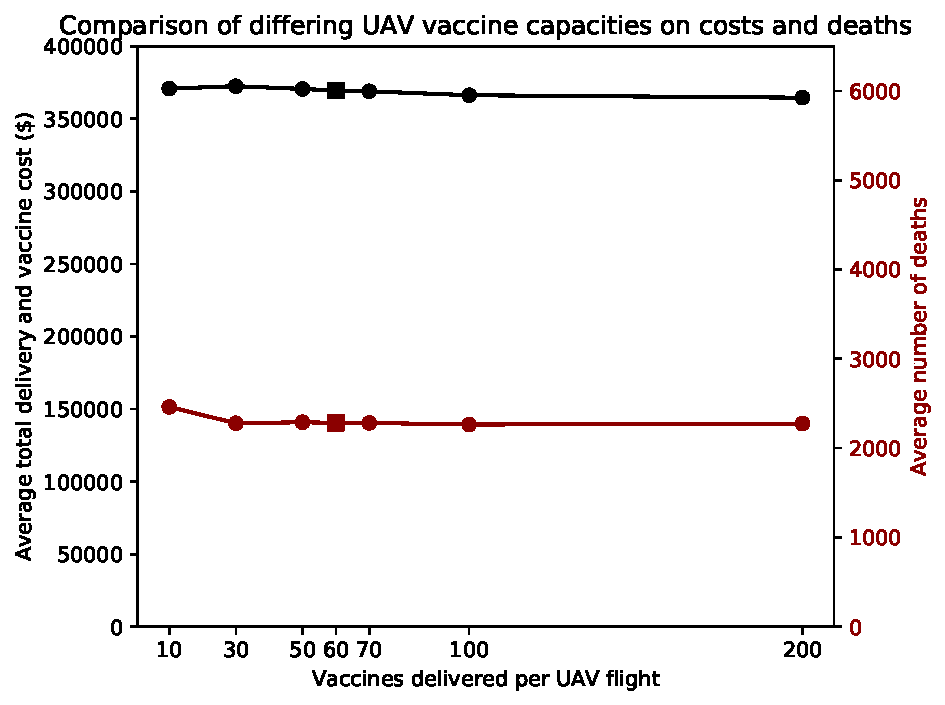
\includegraphics[width=0.47\textwidth, trim={0 0 0 0.67cm}, clip]{Figures/UAVcapacity.pdf}
   \label{fig:res_UAVcap}
 } \vspace{1}
\subfloat[Effect of differing primary vehicle    capacities on results.]{
   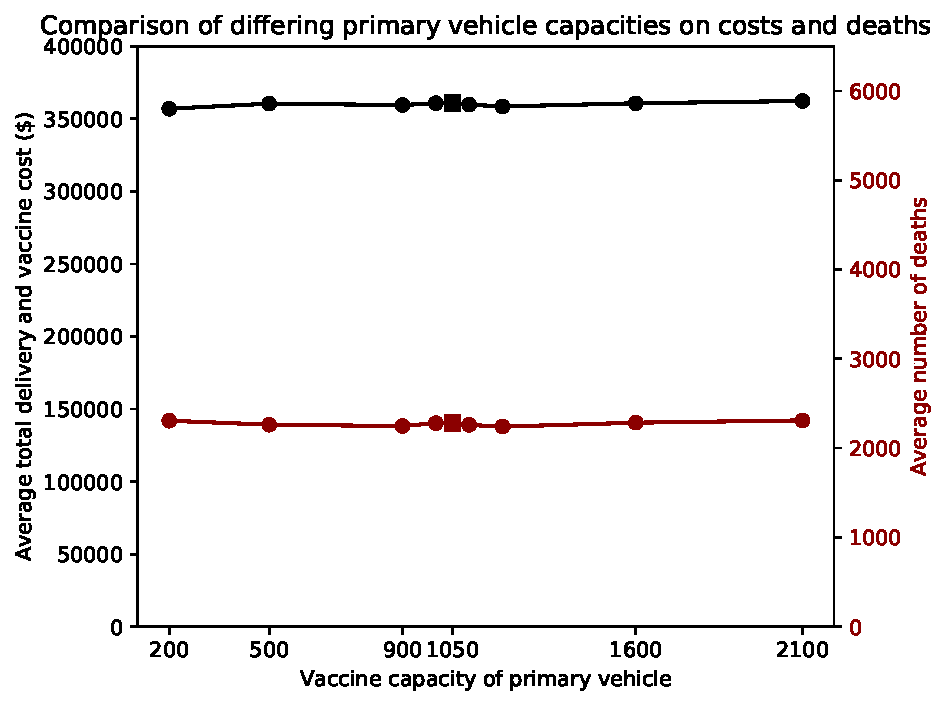
\includegraphics[width=0.47\textwidth, trim={0 0 0 0.67cm}, clip]{Figures/primVehCap.pdf}
   \label{fig:res_primVehCap}
} \hspace{1}
\subfloat[Effect of differing secondary vehicle capacities on results.]{
   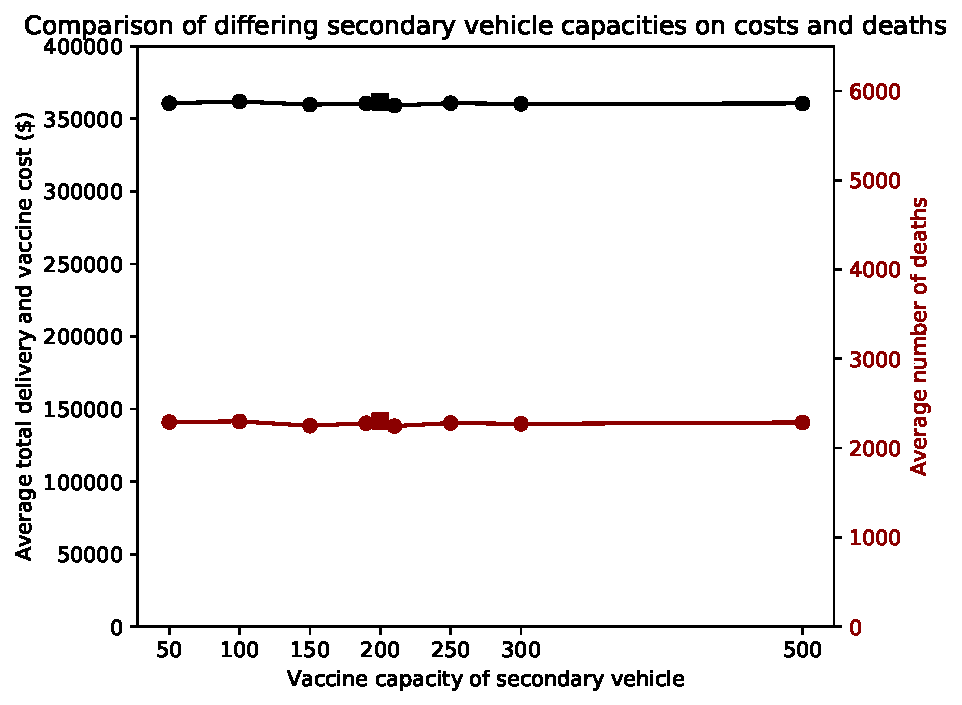
\includegraphics[width=0.47\textwidth, trim={0 0 0 0.67cm}, clip]{Figures/secVehCap.pdf}
   \label{fig:res_secVehCap}
 } \vspace{1}
\subfloat[Effect of cutoff values for combined delivery network on results.]{
   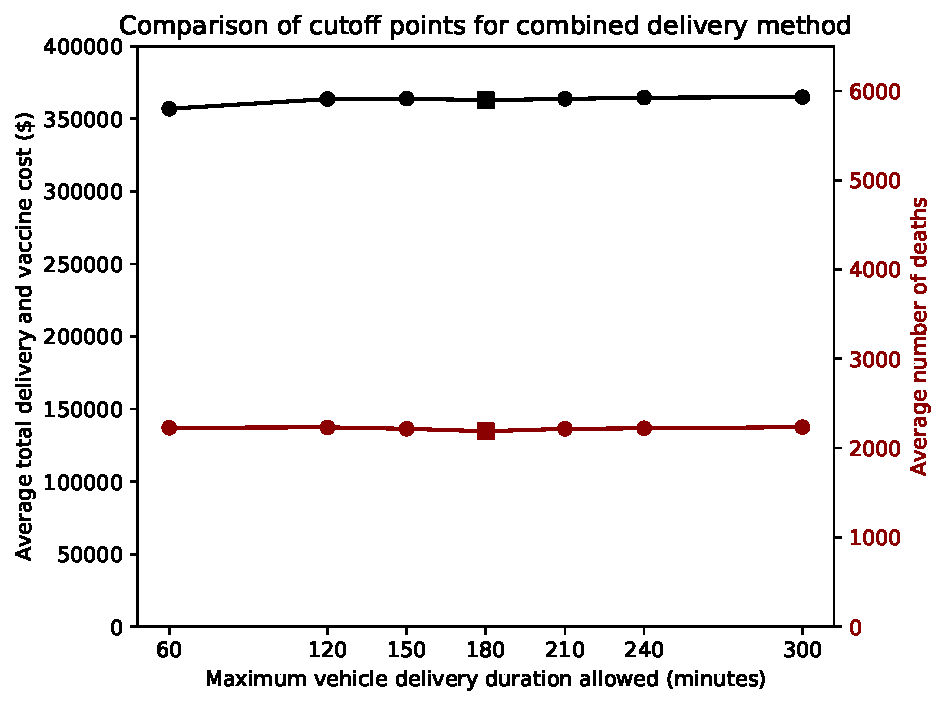
\includegraphics[width=0.47\textwidth, trim={0 0 0 0.67cm}, clip]{Figures/combinedCutoffMins.pdf}
   \label{fig:res_comboCutoff}
 }
\label{fig:deliverySensitivity}
\caption{Comparison of values for delivery-related parameters.}
\end{figure}

\section{Scenario Tests}
\label{sec:res_scenTests}
The factors in an epidemic intervention that can be controlled by decision makers include decisions about who to vaccinate, teams, and intervention timing.

\subsection{Vaccination targeting}
\begin{table}[ht!]
\centering
\begin{tabular}{|c|c|c|}
\hline
\textbf{Metric}  & \multicolumn{1}{c|}{\textbf{Targeted Vaccination}} & \textbf{Untargeted Vaccination} \\ \hline
Deaths           & 2\,212                                             & 4\,218                          \\ \cline{1-1}
Cost             & \$362\,523                                         & \$596\,345                      \\ \cline{1-1}
Vaccinations     & 121\,691                                            & 187\,656                        \\ \cline{1-1}
Vaccines Expired & 4\,969                                             & 17\,239                         \\ \hline
\end{tabular}
\caption{Comparison of targeted vaccination with untargeted vaccination, with values obtained from 500 simulations using each policy.}
\label{tab:res_targetedVacc}
\end{table}

Recall that vaccination can either be targeted (where only those individuals without a previous history of vaccination are vaccinated) or untargeted (where everybody is vaccinated, regardless of vaccination history). Interventions with targeted vaccination are generally more effective since vaccines are only given to those who actually need them, but a drawback of this policy is that documentation about vaccination history may not be available, and that it is usually easier in outbreak response to vaccinate non-selectively. Table \ref{tab:res_targetedVacc} contains the average results of a comparison between the two policies, with each simulated 500 times. Standard deviation is low in both cases. As is clear in the table, there are nearly double the amount of deaths in the case of untargeted vaccination, since a lot of vaccines are `wasted' on already-immune individuals. Without these wasted vaccines, the average cost of targeted vaccination is 39.2\% less than untargeted vaccination. Thus, it is clear that targeted vaccination is significantly better in epidemic response, and dramatically reduces costs and deaths.


\subsection{Team-related parameters}
Vaccination teams are perhaps the most important part of an epidemic response. It is essential to send teams to locations such that the right people are vaccinated on time, in order to curb the epidemic. Three team-related factors can be adjusted in the simulation model:

\begin{itemize}
    \item \textit{The number of (on-duty) vaccination teams in the entire network.} This is set to a constant value of 15 teams initially. The number of teams in the network varies significantly according to the severity of an outbreak, so there is no established, constant number of teams. In a 2016 cholera outbreak response in Zambia, there was a maximum of 17 teams used across 10 locations \cite{poncin2018implementation}, a case similar to the considered network, so 15 is a good general estimate. This is simulated for values ranging from 5 to 25, the results of which can be seen in Figure \ref{fig:vaccTeams}. The figure has two axes; black for average total vaccination and delivery cost incurred, and red for the average number of deaths. Each point is the average result of 500 simulations with that point's number of teams, and the point for the initial value of the number of teams is marked with a square instead of a circle. It is clear that the number of teams in the network has a large impact on the number of deaths and the cost, although this impact decreases as more teams are added. Note that the cost plotted is only the delivery and vaccine cost, and does not include any costs for teams or volunteers. Therefore, since having more teams certainly would incur additional costs, a tradeoff needs to be made, with the number of teams used limited.
    
    \begin{figure}[ht!]{\textwidth}
    \centering
     \subfloat[Comparison of differing numbers of teams.]{
       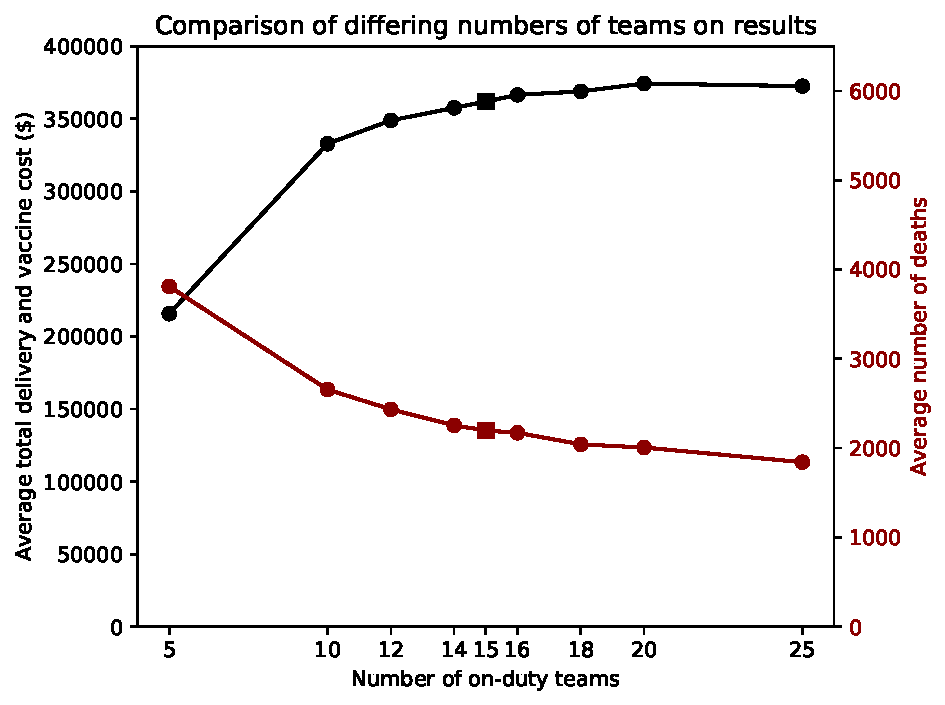
\includegraphics[width=0.48\textwidth, trim={0 0 0 0.67cm}, clip]{Figures/NumberTeams.pdf}
       \label{fig:vaccTeams}
     }
     \subfloat[Comparison of differing daily working minutes.]{
       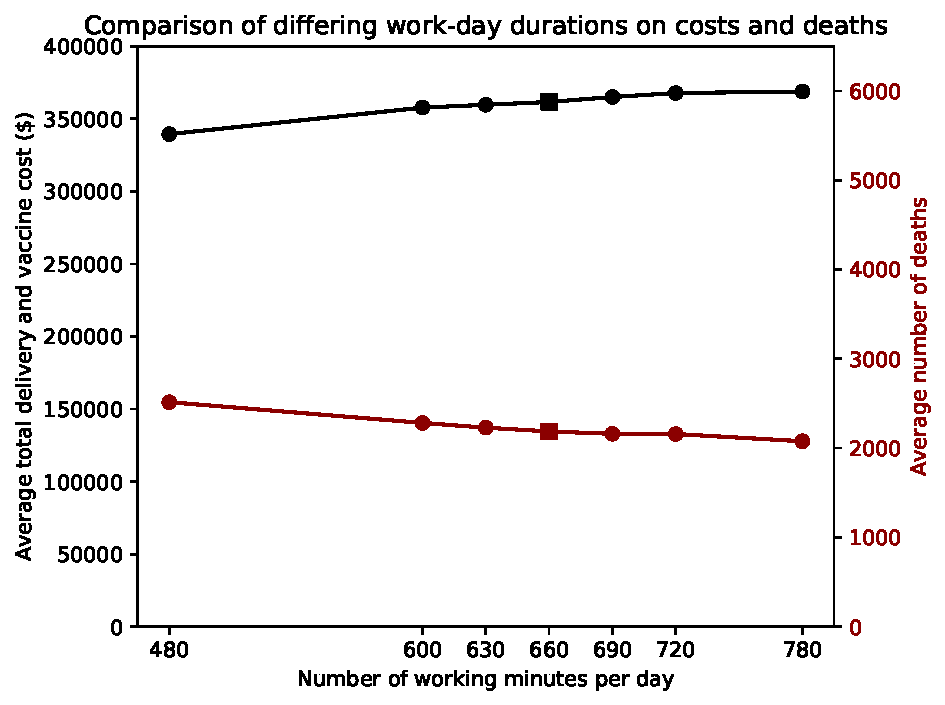
\includegraphics[width=0.48\textwidth, trim={0 0 0 0.67cm}, clip]{Figures/NumberMinsday.pdf}
       \label{fig:vaccMins}
     }
     \vspace{2}
     \subfloat[Comparison of differing weekly working days.]{
       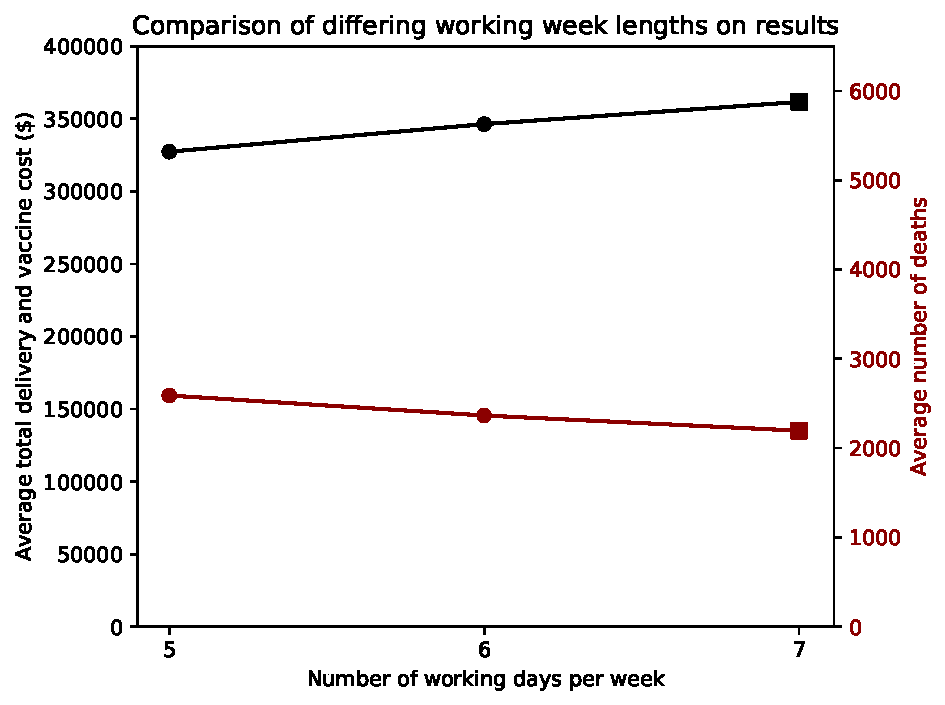
\includegraphics[width=0.48\textwidth, trim={0 0 0 0.67cm}, clip]{Figures/NumberDaysweek.pdf}
       \label{fig:teamWorkDays}
     }
    \caption{Effects of differing values for team-related parameters on cost and deaths.}
    \end{figure}
    
    \item \textit{The number of working minutes for vaccination teams and deliveries per day.} This value is initially set to 660, corresponding to an 11 hour working day \cite{poncin2018implementation}, but is varied between 480 and 780 (8 hours and 13 hours, respectively), producing the results depicted in Figure \ref{fig:vaccMins}. There is a visible impact of the number of minutes worked per day on the number of total deaths and cost; as daily minutes worked increases, the number of deaths decreases. In fact, for each minute above 480 worked each day, the number of deaths reduces by an average of 1.46, while the cost increases by \$97.86. Therefore, working for as long as possible each day is essential, particularly at the crucial beginning stages of the intervention.
    \item \textit{The number of working days for vaccination teams and deliveries per week.} Initially, a full working week of 7 days is assumed. This can be accomplished by having teams working on shifts, so that some teams are able to take time off while others continue to vaccinate. There is simply assumed to be a constant number of 15 teams on duty, 7 days a week. That way, any number of teams can be off duty, as long as 15 are working. To account for 6-day or 5-day work weeks, where on the day(s) off neither deliveries nor vaccinations occur, days are randomly chosen to be taken off with a probability of $\frac{6}{7}$, or $\frac{5}{7}$, respectively. As can be seen in Figure \ref{fig:teamWorkDays}, there is a significant difference in the number of deaths if fewer than 7 days are worked per week. Working 6 days a week instead of 7 results in an average of 170 more deaths, and working 5 days instead of 7 causes an average of 394 more.
    
    To test whether overlapping shifts are significantly better than all teams having a shared day off, two simulations are repeated 500 times each. The first is an intervention with 14 teams, 6 days per week. The second is one with 12 teams, working 7 days per week. Note the total hours worked is the same in both cases, yet the case with 12 teams in overlapping shifts reduces average deaths by nearly 20. The results of this comparison are shown in Table \ref{tab:shiftsVs6days}. Performing a hypothesis test to compare these two deaths means for equality concludes that the null hypothesis (that they are equal) is rejected, with a p-value of less than 0.0001 -- the 95\% confidence interval of the difference between the two is \{-20.9111, -16.2889\}. Thus, overlapping shifts are significantly better than shared days off, in the simulations conducted.
    
    \begin{table}[ht!]
    \centering
    \resizebox{\textwidth}{!}{%
    \begin{tabular}{|cc|ccc|}
    \hline
    \multicolumn{1}{|c|}{Number of teams on duty} & Work days per week & \multicolumn{1}{c|}{Average deaths} & \multicolumn{1}{c|}{Average cost} & Average vaccines spoiled \\ \hline
    14 & 6 & 2453.3 & 340\,512 & 6807.8 \\
    12 & 7 & 2434.7 & 348\,866 & 6474.7 \\ \hline
    \end{tabular}%
    }
    \caption{Comparison of overlapping shifts against all teams having a common day off}
    \label{tab:shiftsVs6days}
    \end{table}
    
    \item \textit{The number of vaccinations that teams can perform daily.} This value is initially set to 450 vaccinations per day for fixed-post teams, and to 250 for mobile teams, as in \S \ref{meth:MeaslesCompa}. These values are each ranged between 100 and 800, and 50 and 450, respectively; with results plotted in Figures \ref{fig:fixedVaccAbility} and \ref{fig:mobileVaccAbility}. It is obvious in the figures that if each fixed-post team could vaccinate more people daily, the intervention would be able to reduce the average total deaths considerably. The same does not hold for mobile teams; there is hardly any impact of changes in teams' abilities to vaccinate, although this is largely a result of the considered network being mostly urban areas (so, using more fixed teams).
    
    \begin{figure}[ht!]{\textwidth}
    \centering
     \subfloat[Comparison of fixed-post teams' daily ability to vaccinate.]{
       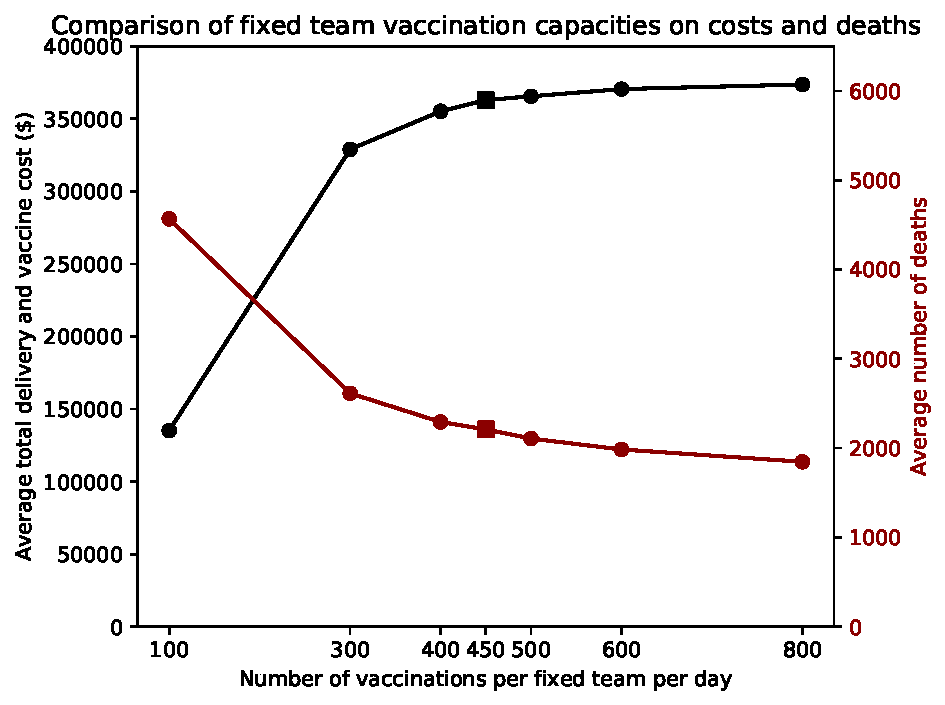
\includegraphics[width=0.48\textwidth, trim={0 0 0 0.67cm}, clip]{Figures/fixedVaccAbility.pdf}
       \label{fig:fixedVaccAbility}
     }
     \vspace{2}
     \subfloat[Comparison of mobile teams' daily ability to vaccinate.]{
       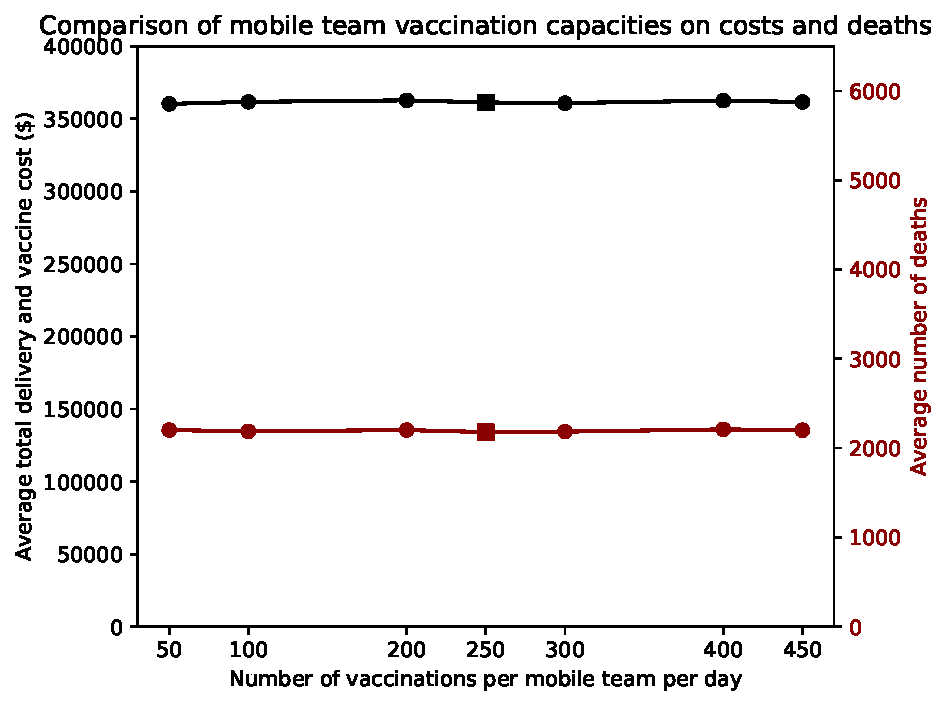
\includegraphics[width=0.48\textwidth, trim={0 0 0 0.67cm}, clip]{Figures/mobileVaccAbility.pdf}
       \label{fig:mobileVaccAbility}
     }
    \caption{Comparing results of different team abilities for vaccinations per day.}
    \end{figure}
    
\end{itemize}

\subsection{Intervention timing parameters}
The final set of parameters that decision makers can vary involve aspects of intervention timing. It is well known that the earlier an intervention begins, the more effective it will be, and this is confirmed by the results found, along with two other important results. The following parameters are tested for differing values:

\begin{itemize}
    \item \textit{The proportion of the population at any location to be infected before an epidemic is declared.} A simple method of declaring the epidemic is used for this project; once the ratio of infectious individuals to the population in any area exceeds a certain threshold (this parameter value), the epidemic is declared, and preparations begin for the intervention to start. An initial proportion of 0.5\% is used. This method is intuitive, because the higher the proportion of infections to population, the more noticeable the infections will be to local health workers, and so the epidemic would be declared. Different values of this threshold are plotted as percentages in Figure \ref{fig:intThres}. Clearly, the simulation output is very sensitive to changes in this threshold. The longer it takes for an epidemic to be declared and for vaccinations to begin, the more deaths. Practically, this detection threshold could be improved by educating local health workers to recognise measles cases better, and to understand the risks of measles. It is difficult to estimate what an accurate value for this threshold would be. Comparing real-life epidemic detection methods is a useful topic for future research.
    
    \begin{figure}[ht!]{\textwidth}
    \centering
     \subfloat[Comparison of epidemic declaration thresholds.]{
       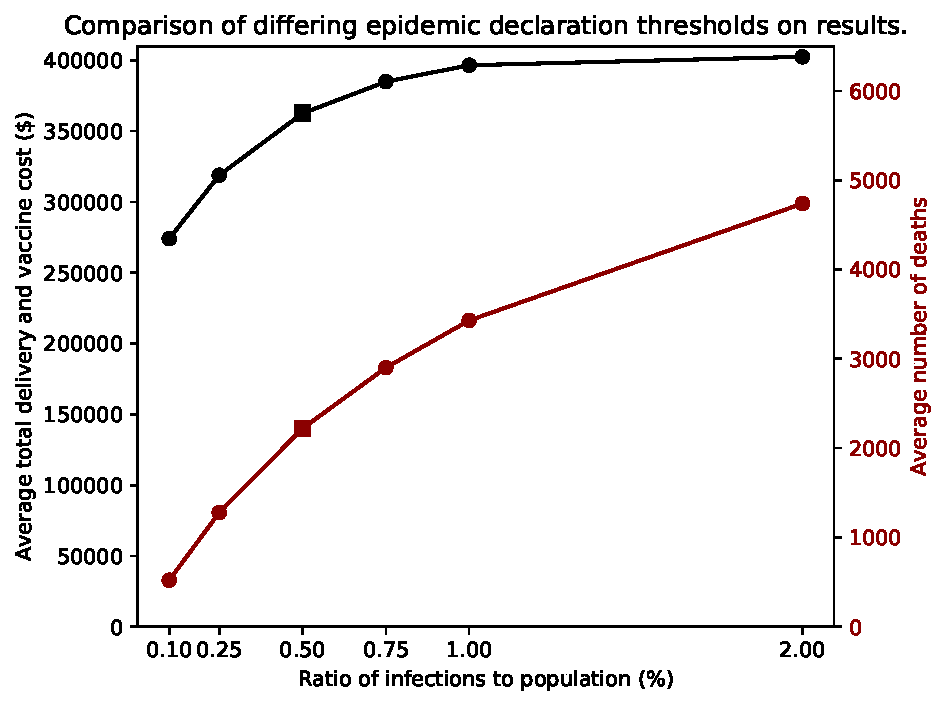
\includegraphics[width=0.48\textwidth, trim={0 0 0 0.67cm}, clip]{Figures/IntThreshold.pdf}
       \label{fig:intThres}
     }
     \subfloat[Comparison of differing intervention delays.]{
       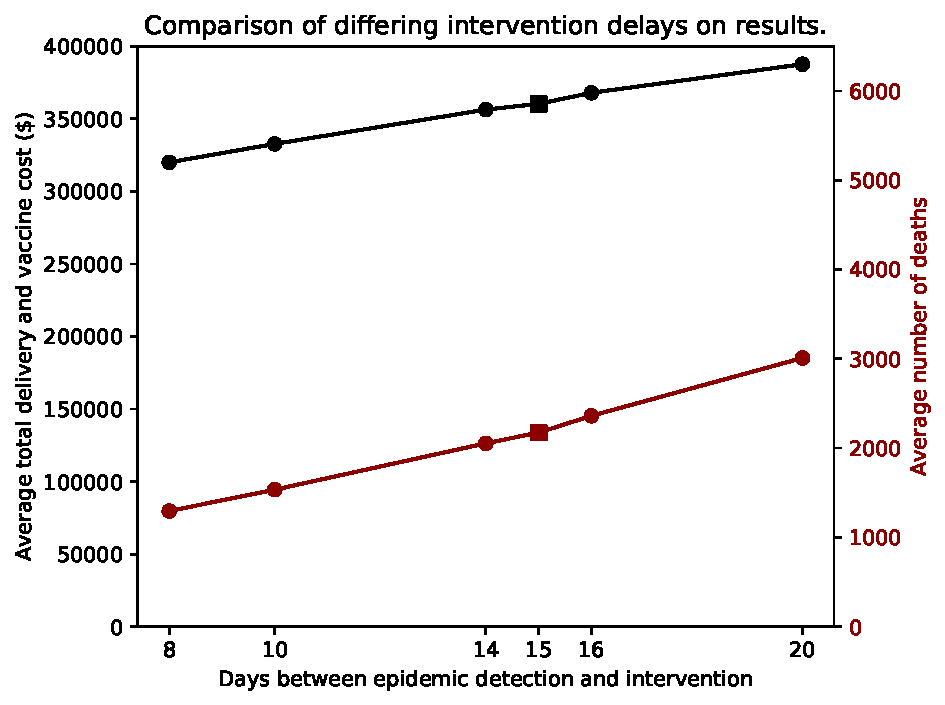
\includegraphics[width=0.48\textwidth, trim={0 0 0 0.67cm}, clip]{Figures/IntLeadTime.pdf}
       \label{fig:intLeadTime}
     }
     \vspace{2pt}
     \subfloat[Comparison of differing intervention lengths.]{
       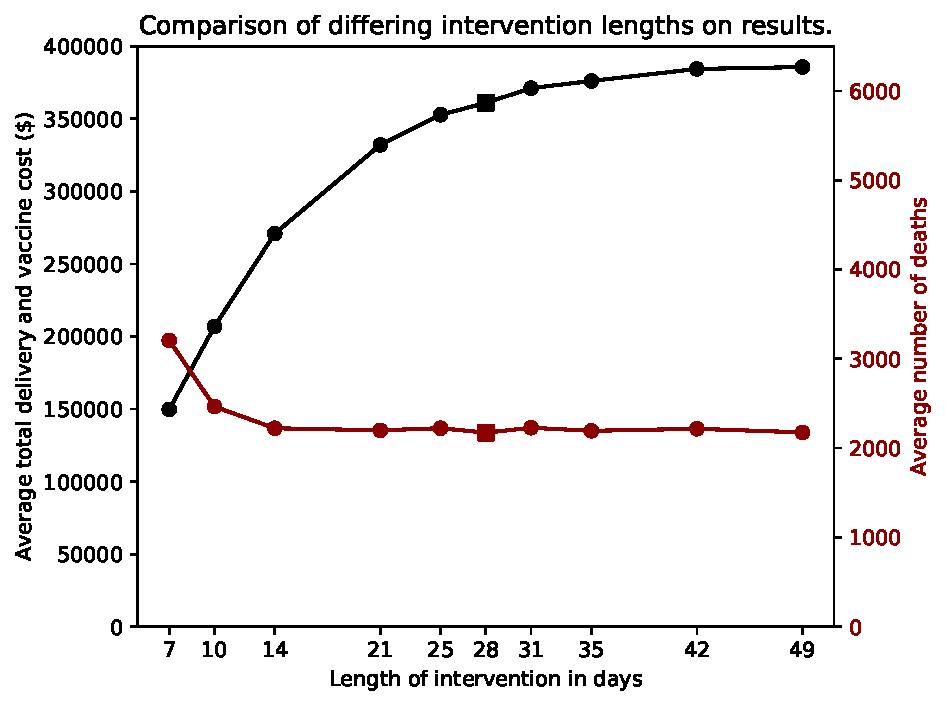
\includegraphics[width=0.48\textwidth, trim={0 0 0 0.67cm}, clip]{Figures/IntLength.pdf}
       \label{fig:intLength}
     }
    \caption{Effects of differing values for team-related parameters on cost and deaths.}
    \end{figure}
    
    \item \textit{The number of days after the epidemic has been detected, until intervention begins.} MSF states that,
    "emergency vaccination campaign preparation should not take more than two weeks," and that, "ideally, emergency vaccination activities can be set up in 8 to 10 days, 15 days maximum" 
    \cite{danet_fermon_2013}. The delay before intervention is a much-discussed topic in epidemic response, and although it is well known that the response needs to be as prompt as possible, it is often difficult to set up the delivery network and get teams on the ground more quickly. Were a UAV network to be used in the future, it would need to be set up from scratch within 8-10 days, ideally. As can be seen in Figure \ref{fig:intLeadTime}, the number of deaths increases in a linear fashion as the delay increases. For each extra day of delay above 8, there is a simulated average of 143 more deaths.
    
    \item \textit{Length of intervention in days.} The length of an intervention depends largely on the severity of an epidemic, and so, the results depicted in Figure \ref{fig:intLength} apply specifically to the case of this measles outbreak. An initial length of 28 days is used so that strategies can be compared for long enough. A useful result shown in the figure is that although vaccinations continue after day 14 (and costs continue to rise), the number of deaths does not decrease. This is likely because nearly all of the susceptible individuals in the network can be vaccinated within 14 days with a good team allocation. Even after 7 days of intervention, the average total number of deaths (3206) is less than half of what it would've been without an intervention (6504).
\end{itemize}

\chapter{Conclusion}
This report introduced the problems faced by current outbreak response interventions, and the possibility of using UAVs in rural areas for humanitarian aid deliveries. The properties of measles and the method in which it is often simulated -- the compartmental model -- are also introduced. A short review of relevant literature and similar work is performed in Chapter 2, introducing methods that are used for the simulation. The methodology used to construct the simulation model in Python is presented in Chapter 3, which is followed by a detailed discussion on results obtained in Chapter 4. The results found in Chapter 4 provide some useful insight into improving epidemic response, with particular focus on the case of measles outbreaks in rural areas. The project was able to achieve all five objectives outlaid in the introduction; a review of relevant literature was conducted, and a simulation of a measles epidemic in a network was developed. The expected prevented exposures model was formulated and implemented for resource allocation decisions, and heuristic strategies for resource allocation were discussed and investigated. Finally, UAVs were evaluated as a vaccine delivery method, and certain other improvements to interventions were found.

In the sensitivity analysis performed on uncontrollable parameters, the model was found to be most sensitive to changes in $R_{0}$, and durations of exposure and infection. Among the controllable improvements found are aspects regarding teams, delivery methods, and the timing of the intervention. As the number of teams in the network increases, the number of deaths decreases, but this decrease reduces as even more teams are added. Since there is a tradeoff between cost and assigning more teams, 12-18 teams are recommended for a network such as the one investigated. However, this only applies to the case study considered; better methods for determining a good number of teams in general, pose potential for future work. Teams' working hours per day also play an important role; it was found that, on average in the whole vaccination network, for each minute above 8 hours worked daily, there are 1.46 deaths prevented. Further, having teams working in overlapping shifts rather than having a shared day off was shown to reduce deaths significantly. 

In repeated testing, simulations showed that the team allocation strategy employed has a much larger impact on the intervention than the choice of where to deliver vaccines to once teams are already placed. For the network tested, the strategy of sending teams to locations proportionally to those locations' populations was found to be the most effective team allocation method for reducing deaths, without considering cost. However, the best performing strategy when both deaths and cost are considered, was found to be the optimal expected prevented exposures strategy developed using linear programming. This strategy, compared to the population strategy, reduced average cost by \$81\,016 (a 22.4\% reduction), while only increasing the average number of deaths by 0.9\%, an almost negligible amount (although this may be significant, depending on the decision-maker). This EPE strategy, and the use of simulation during outbreak response to support decision-making, provides invaluable potential for improvement in interventions.

With regard to vaccine delivery methods, UAVs were shown to be able to meet demand for vaccines entirely, and are on par with vehicle delivery networks when 3 or more UAVs are used. Under the assumption that each UAV flight costs \$17, UAV delivery is cheaper than land-based delivery in areas with poor road infrastructure, and also reduces the average number of deaths. The percentage of roads impassable for which it is better to use UAVs than vehicles was estimated to be 12.5\%, based on the network used as a case study -- i.e. if any more than 12.5\% of roads in a network are impassable, UAVs would be cheaper and more effective than vehicles for vaccine delivery in the case of an outbreak. This percentage, however, only applies to the case study considered, and further research into a general percentage based on a range of different network structures is required.

UAVs with an average speed below 80 km/h or a capacity of below 30 vaccines were found to increase the average number of deaths, while all UAVs above these levels had almost identical performance. Therefore, these minimum standards need to be met for a UAV to suffice for a vaccine delivery network such as the one modelled. 
For the case study considered, the combination of one primary vehicle and one secondary, smaller vehicle were found to be sufficient for delivering vaccines on time. Further, results indicate that the measles vaccine would only need to remain potent for one day outside of the cold chain to maintain similar intervention success -- there is no improvement in the number of deaths if the vaccine lasts longer, although it would simplify deliveries and slightly reduce delivery cost.

Aside from team allocation, the most important aspects of epidemic response were found to be early detection, and swift, focused response. For each day longer than MSF's recommended 8 day response delay (the time between epidemic detection and the beginning of vaccinations), an average of 143 deaths was caused. It is thus imperative to reduce the time it takes to set up an intervention. Further, reducing migration by discouraging movement between locations in the network was shown to have a slight impact on the spread of the epidemic, albeit not as significant as better team allocations and earlier intervention. Finally, using targeted vaccination instead of untargeted, non-selective vaccination, was shown to almost halve the number of deaths and reduce cost by 39.2\%.

Other possible opportunities for future work include more realistic modelling of vehicle deliveries, with more intelligently selected routes, as well as better modelling of migration; perhaps using the radiation model instead of the gravity model. Agent-based simulation could be used to gain a different and more low-level insight into resource allocation strategies, and more team allocation strategies could be evaluated. If more comprehensive data can be gathered about another historical measles outbreak, the model can be validated on a different case study, and historical interventions can be compared with those tested and formulated in this report. Alternatively, a large number of networks could be generated programmatically for validation (and better determination of the percentage of closed roads for which it is beneficial to use UAVs instead of vehicles), allowing the effect of different network structures on the resource allocation models to be seen. Furthermore, global sensitivity analysis methods, such as partial rank correlation coefficients, could be implemented.

To reiterate the conclusions drawn and answer the research question posed in the introduction; UAVs were able to successfully meet vaccine demand in simulations, and reduced costs and deaths in cases where road quality was poor. Furthermore, the use of the EPE team allocation strategy with targeted vaccination, and having shorter intervention delays, were found to be the most significant factors in improving intervention success.

\bibliographystyle{orion_and}
%\cleardoublepage
\addcontentsline{toc}{chapter}{Bibliography}
\bibliography{refs}
%You need to look at the Referencing.pdf document on Sunlearn to ensure all references are correctly formatted

%\cleardoublepage
\addcontentsline{toc}{chapter}{Appendix}
\appendix
\chapter{Simulation Output}
\label{app:simOut}

Tables \ref{tab:vehicle_stratPairs}, \ref{tab:UAV_stratPairs}, and \ref{tab:Combined_stratPairs} are all in the same format, and contain simulation results for 500 simulations of interventions with vehicle deliveries, UAV deliveries and a combination of both types, respectively. The average values for Deaths and Cost are rounded to the nearest integer.

\begin{table}[ht!]
\centering
\resizebox{\textwidth}{!}{%
\begin{tabular}{c|c|c|c|c|c|c|c|c|c|c|c|c|}
\cline{2-13}
 & \multicolumn{12}{c|}{Team  Allocation Strategy} \\ \cline{2-13} 
 & \multicolumn{2}{c|}{S} & \multicolumn{2}{c|}{I} & \multicolumn{2}{c|}{I/N} & \multicolumn{2}{c|}{Spread} & \multicolumn{2}{c|}{N} & \multicolumn{2}{c|}{EPE} \\ \hline
\multicolumn{1}{|c|}{\begin{tabular}[c]{@{}c@{}}Vaccine delivery \\ strategy\end{tabular}} & Deaths & Cost & Deaths & Cost & Deaths & Cost & Deaths & Cost & Deaths & Cost & Deaths & Cost \\ \hline
\multicolumn{1}{|c|}{I} & 2214 & 313015 & 2193 & 374497 & 3919 & 181579 & 4518 & 128945 & 2212 & 362523 & 2217 & 280979 \\ \cline{1-1}
\multicolumn{1}{|c|}{S} & 2210 & 315931 & 2217 & 375791 & 3915 & 181326 & 4534 & 128489 & 2216 & 362801 & 2204 & 280735 \\ \cline{1-1}
\multicolumn{1}{|c|}{N} & 2201 & 312711 & 2205 & 375372 & 3934 & 181577 & 4513 & 128953 & 2184 & 361751 & 2237 & 280786 \\ \cline{1-1}
\multicolumn{1}{|c|}{EPE} & 2224 & 317410 & 2200 & 375490 & 3930 & 182129 & 4516 & 132264 & 2193 & 362290 & 2227 & 281332 \\ \hline
\end{tabular}
}
\caption{Average number of deaths and total cost of different strategy pairs for vehicle deliveries.}
\label{tab:vehicle_stratPairs}
\end{table}

\begin{table}[ht!]
\centering
\resizebox{\textwidth}{!}{%
\begin{tabular}{c|c|c|c|c|c|c|c|c|c|c|c|c|}
\cline{2-13}
 & \multicolumn{12}{c|}{Team  Allocation Strategy} \\ \cline{2-13} 
 & \multicolumn{2}{c|}{S} & \multicolumn{2}{c|}{I} & \multicolumn{2}{c|}{I/N} & \multicolumn{2}{c|}{Spread} & \multicolumn{2}{c|}{N} & \multicolumn{2}{c|}{EPE} \\ \hline
\multicolumn{1}{|c|}{\begin{tabular}[c]{@{}c@{}}Vaccine delivery \\ strategy\end{tabular}} & Deaths & Cost & Deaths & Cost & Deaths & Cost & Deaths & Cost & Deaths & Cost & Deaths & Cost \\ \hline
\multicolumn{1}{|c|}{I} & 2311 & 325608 & 2203 & 376258 & 3895 & 196581 & 4555 & 140089 & 2204 & 364479 & 2280 & 286526 \\ \cline{1-1}
\multicolumn{1}{|c|}{S} & 2321 & 325669 & 2242 & 378343 & 3979 & 189166 & 4605 & 136885 & 2252 & 363925 & 2311 & 285438 \\ \cline{1-1}
\multicolumn{1}{|c|}{N} & 2316 & 324547 & 2222 & 377632 & 3981 & 192240 & 4616 & 140762 & 2229 & 361833 & 2326 & 287541 \\ \cline{1-1}
\multicolumn{1}{|c|}{EPE} & 2343 & 283794 & 2207 & 350188 & 3829 & 177802 & 4570 & 116032 & 2216 & 343145 & 2320 & 277131 \\ \hline
\end{tabular}
}
\caption{Average number of deaths and total cost of different strategy pairs for UAV deliveries.}
\label{tab:UAV_stratPairs}
\end{table}

\begin{table}[ht!]
\centering
\resizebox{\textwidth}{!}{%
\begin{tabular}{c|c|c|c|c|c|c|c|c|c|c|c|c|}
\cline{2-13}
 & \multicolumn{12}{c|}{Team  Allocation Strategy} \\ \cline{2-13} 
 & \multicolumn{2}{c|}{S} & \multicolumn{2}{c|}{I} & \multicolumn{2}{c|}{I/N} & \multicolumn{2}{c|}{Spread} & \multicolumn{2}{c|}{N} & \multicolumn{2}{c|}{EPE} \\ \hline
\multicolumn{1}{|c|}{\begin{tabular}[c]{@{}c@{}}Vaccine delivery \\ strategy\end{tabular}} & Deaths & Cost & Deaths & Cost & Deaths & Cost & Deaths & Cost & Deaths & Cost & Deaths & Cost \\ \hline
\multicolumn{1}{|c|}{I} & 2215 & 333434 & 2213 & 375683 & 3728 & 208920 & 4513 & 137884 & 2220 & 364370 & 2241 & 281764 \\ \cline{1-1}
\multicolumn{1}{|c|}{S} & 2190 & 333093 & 2206 & 375210 & 3734 & 209047 & 4510 & 138409 & 2213 & 363961 & 2215 & 281649 \\ \cline{1-1}
\multicolumn{1}{|c|}{N} & 2208 & 333461 & 2181 & 374412 & 3697 & 210235 & 4519 & 138583 & 2218 & 364035 & 2223 & 282259 \\ \cline{1-1}
\multicolumn{1}{|c|}{EPE} & 2199 & 323589 & 2211 & 374845 & 3704 & 202595 & 4500 & 129720 & 2207 & 361129 & 2216 & 280085 \\ \hline
\end{tabular}%
}
\caption{Average deaths and cost of different strategy pairs for a combined delivery network.}
\label{tab:Combined_stratPairs}
\end{table}

Table \ref{tab:combiSims} contains simulation results (the average of deaths and cost from 500 simulations) for different numbers of UAVs and vehicles used in the combined delivery strategy. The case where there are either 0 UAVs or 0 vehicles is excluded since that would be a UAV-only or vehicle-only network.

\begin{table}[t!]
\centering
\begin{tabular}{|c|c|c|c|}
\hline
\multicolumn{1}{|c|}{Vehicles} & UAVs & \multicolumn{1}{c|}{Average Deaths} & Average Cost \\ \hline
1 & 1 & 2215 & 364082 \\
2 & 1 & 2211 & 363611 \\
2 & 2 & 2220 & 364548 \\
1 & 2 & 2228 & 365087 \\
3 & 1 & 2190 & 362540 \\
1 & 3 & 2205 & 364064 \\
3 & 3 & 2199 & 363459 \\
5 & 5 & 2201 & 363853 \\ \hline
\end{tabular}%

\caption{Comparison of different numbers of vehicles and UAVs in the combined delivery strategy.}
\label{tab:combiSims}
\end{table}

\end{document}